\documentclass[a4paper,11pt]{article}

% ------------------------------
% Geometry and Page Layout
% ------------------------------
\usepackage{geometry}
\geometry{left=1in, right=1in, top=1in, bottom=1in} % Set 1-inch margins
\usepackage{fancyhdr}   % Header and footer customization
\usepackage{pdflscape}  % Landscape pages
\usepackage{everypage}  % Add hooks to every page

% ------------------------------
% Font and Typography
% ------------------------------
\usepackage{mathptmx}   % Use Times New Roman font (or Computer Modern by default)
\renewcommand{\baselinestretch}{1.5} % Line spacing
\usepackage[utf8]{inputenc} % UTF-8 support
\usepackage{tocloft}
\usepackage[normalem]{ulem}

% ------------------------------
% For customizing titles
% ------------------------------
\usepackage{titlesec}
% Redefine \section to be unnumbered but still included in TOC
\titleformat{\section}[hang]{\centering\normalfont\Large\bfseries}{}{0pt}{} % Removes numbering from section titles

% ------------------------------
% Date Handling
% ------------------------------
\usepackage[english]{datetime2}
\DTMnewdatestyle{mydateA}{%
  \renewcommand*{\DTMdisplaydate}[4]{%
    \DTMtwodigits{##3}/\DTMtwodigits{##2}/##1}%
  \renewcommand*{\DTMDisplaydate}{\DTMdisplaydate}%
}
\DTMnewdatestyle{mydateB}{%
  \renewcommand*{\DTMdisplaydate}[4]{%
    \DTMtwodigits{##3} \DTMenglishmonthname{##2} ##1}%
  \renewcommand*{\DTMDisplaydate}{\DTMdisplaydate}%
}

% ------------------------------
% Color and Graphics
% ------------------------------
\usepackage[table]{xcolor}
\definecolor{mygreen}{rgb}{0.82, 0.94, 0.75}
\definecolor{mygreen2}{rgb}{0.67, 0.88, 0.69}
\definecolor{codegreen}{rgb}{0,0.94,0}
\definecolor{codegray}{rgb}{0.5,0.5,0.5}
\definecolor{codepurple}{rgb}{0.58,0,0.82}
\definecolor{backcolour}{rgb}{0.95,0.95,0.92}
\usepackage{graphicx}   % For including figures
\graphicspath{{}}       % Set graphic paths
\DeclareGraphicsExtensions{.pdf,.jpeg,.png,.jpg}
\usepackage{tikz}       % For custom drawings and diagrams
\usepackage{subcaption}  % For subfigures
\usepackage{float}

% ------------------------------
% Mathematics
% ------------------------------
\usepackage{amsmath}    % Mathematical symbols and environments
\usepackage{amssymb}    % Additional math symbols
\usepackage{yhmath}     % Extended math fonts
\usepackage{extarrows}  % Extensible arrows
\usepackage{esint}      % Integrals
\usepackage{bigints}    % Large integral symbols
\usepackage{mathrsfs}   % Script math font

% ------------------------------
% Code Formatting
% ------------------------------
\usepackage{listings}   % Code listings
\lstdefinestyle{mystyle}{
    backgroundcolor=\color{backcolour},   
    commentstyle=\color{green!50!black},
    keywordstyle=\color{blue},
    numberstyle=\tiny\color{codegray},
    stringstyle=\color{red},
    basicstyle=\ttfamily\footnotesize, % Adjusting the code size here
    breakatwhitespace=false,         
    breaklines=true,                 
    captionpos=b,                    
    keepspaces=true,                 
    numbers=left,                    
    numbersep=5pt,                  
    showspaces=false,                
    showstringspaces=false,
    showtabs=false,                  
    tabsize=2,
    frame=single,
    captionpos=b
}
\lstset{style=mystyle}

% ------------------------------
% Bibliography Management
% ------------------------------
\usepackage[
            backend=biber, 
            isbn=false, 
            url=true, 
            doi=true, 
            giveninits=true, 
            sorting=nyt]{biblatex}
\addbibresource{ref.bib}

% Optional: Customize title formatting to keep hyperlinks intact
\newbibmacro{string+doi}[1]{%
  \iffieldundef{doi}{#1}
  {\href{https://doi.org/\thefield{doi}}{#1}}}

\DeclareFieldFormat{title}{\usebibmacro{string+doi}{\mkbibemph{#1}}}
\DeclareFieldFormat[article]{title}{\usebibmacro{string+doi}{\mkbibquote{#1}}}
\DeclareFieldFormat[article,periodical]{volume}{\mkbibbold{#1}}
\DeclareFieldFormat[article,periodical]{number}{\mkbibbold{#1}}

% ------------------------------
% Packages for Tables
% ------------------------------
\usepackage{array}      % Extended column definitions
\usepackage{tabularx}   % Table with adjustable-width columns
\usepackage{longtable}  % Tables spanning multiple pages
\usepackage{booktabs}   % Formal tables
\usepackage{arydshln}   % Dashed lines in tables
\usepackage{multirow}   % Multi-row cells
\usepackage{makecell}   % Enhanced table cells
\usepackage{tasks}      % Task lists within tables

% ------------------------------
% Custom Commands and Settings
% ------------------------------
\newcommand{\checkbox}{\makebox[0.5cm]{\strut $\square$}} % Custom checkbox command
\newcommand{\RotatePagenumber}{%
  \ifdim\textwidth=\linewidth
    % Do nothing if text width equals line width
  \else
    \begingroup
    \dimendef\margins=0
    \ifodd\value{page}
      \margins=\oddsidemargin
    \else
      \margins=\evensidemargin
    \fi
    \raisebox{\dimexpr -\topmargin-\headheight-\headsep-\footskip-1cm}[0pt][0pt]{%
      \rlap{\hspace{\dimexpr \margins + \textheight + \footskip + \marginparwidth}%
      \llap{\rotatebox{90}{\thepage}}}}%
    \endgroup
  \fi
}
\AddEverypageHook{\RotatePagenumber} % Apply custom page numbering

% ------------------------------
% Color and Hyperlink Settings
% ------------------------------
\usepackage[colorlinks]{hyperref}
\hypersetup{
    linkcolor=blue,   % Color for internal links
    citecolor=red,    % Color for citations
    urlcolor=purple,  % Color for URLs
}

% ------------------------------
% cross reference
% ------------------------------
\usepackage[nameinlink,capitalize]{cleveref} %cross reference showing Eq. (1) etc.

% ------------------------------
% command to delete the side numbering and add bottom numbering (Function)
% ------------------------------
\newcommand{\Lpagenumber}{\ifdim\textwidth=\linewidth\else\bgroup
  \dimendef\margin=0 %use \margin instead of \dimen0
  \ifodd\value{page}\margin=\oddsidemargin
  \else\margin=\evensidemargin
  \fi
  \raisebox{\dimexpr -\topmargin-\headheight-\headsep-0.5\linewidth}[0pt][0pt]{%
    \rlap{\hspace{\dimexpr \margin+\textheight+\footskip}%
    \llap{\rotatebox{90}{\thepage}}}}%
\egroup\fi}
\AddEverypageHook{\Lpagenumber}%

% ------------------------------
% Start Document
% ------------------------------
\begin{document}
\thispagestyle{empty}
\DTMsetdatestyle{mydateA}

%%%%%%%%%%%%%%%%%%%%%%%%%%%%%%%%%%%%%%%%%%%%%%%%%%%%%%%%%%%%%%%%%%%%%%%%%%%%%%%%%%%%%%%%
% Slip
%%%%%%%%%%%%%%%%%%%%%%%%%%%%%%%%%%%%%%%%%%%%%%%%%%%%%%%%%%%%%%%%%%%%%%%%%%%%%%%%%%%%%%%%
%SCHOOL OF PHYSICS -- LEVEL 200 PHYSICS LABORATORY REPORT SLIP
\begin{center}
    \textbf{SCHOOL OF PHYSICS -- LEVEL 200 PHYSICS LABORATORY REPORT SLIP} \\
    \textbf{FOR ZCT 293/2 AND ZCT 294/2}
\end{center}

\begin{table}[h]
\begin{center}
\resizebox{\textwidth}{!}{
\begin{tabular}{|llllllllllllllllllll|}
\hline
\multicolumn{20}{|l|}{\textbf{Instructions to student:} Please make sure you fill in the form completely.} \\
\multicolumn{20}{|l|}{\textbf{Instructions to lecturer:} Kindly record the numerical marks in the rubric assessment form, not here.} \\ \hline
\multicolumn{20}{|c|}{
  \centering{\textbf{PARTICULARS}}
}                                                                                                                                      \\ \hline
Name & :\,\,TAN WEI LIANG & \multicolumn{18}{l|}{}                                                                                                                                                                        
\\ \hline
Matric no. & :\,\,22302889  & \multicolumn{18}{l|}{}                                                                                                                                                                        
\\ \hline
Group& :\,\,W2  & \multicolumn{18}{l|}{}                                                                                                                                                                        
\\ \hline
Expt. Code & :\,\,2GP2 & \multicolumn{18}{l|}{}                                                                                                                                                                        
\\ \hline
Expt. Title & :\,\,POISSON'S RATIO AND YOUNG'S MODULUS FOR GLASS & \multicolumn{18}{l|}{}                                                                                                                                                                        
\\ \hline
Lecturer in charge & :\,\,DR. ABDUL HADI BIN SULAIMAN & \multicolumn{18}{l|}{}                                                                                                                                                                        
\\ \hline
Report due date & :\,\,23/04/2025 & \multicolumn{18}{l|}{}                                                                                                                                                                        
\\ \hline
\multicolumn{11}{|c|}{\textbf{Experiment (\checkmark)}} & \multicolumn{9}{c|}{\textbf{Lab Report Grade (\checkmark)}} \\ 
\hline
\multicolumn{11}{|c|}{1 $\text{\rlap{$\checkmark$}}\square$ \quad 2 $\square$ \quad 3 $\square$ \quad 4 $\square$ \quad 5 $\square$ \quad 6 $\square$} & 

\multicolumn{1}{l|}{A} & \multicolumn{1}{l|}{$\square$} &
\multicolumn{1}{l|}{A$-$} & \multicolumn{1}{l|}{$\square$} &
\multicolumn{1}{l|}{B$+$} & \multicolumn{1}{l|}{$\square$} &
\multicolumn{1}{l|}{B} & \multicolumn{1}{l|}{$\square$} 
&\multicolumn{1}{l|}{}
\\ \hline
\multicolumn{11}{|l|}{} & 

\multicolumn{1}{l|}{B$-$} & \multicolumn{1}{l|}{$\square$} &
\multicolumn{1}{l|}{C$+$} & \multicolumn{1}{l|}{$\square$} &
\multicolumn{1}{l|}{C} & \multicolumn{1}{l|}{$\square$} &
\multicolumn{1}{l|}{C$-$} & \multicolumn{1}{l|}{$\square$} 
&\multicolumn{1}{l|}{}
\\ \hline

\multicolumn{11}{|c|}{} & 

\multicolumn{1}{l|}{D$+$} & \multicolumn{1}{l|}{$\square$} &
\multicolumn{1}{l|}{D} & \multicolumn{1}{l|}{$\square$} &
\multicolumn{1}{l|}{D$-$} & \multicolumn{1}{l|}{$\square$} &
\multicolumn{1}{l|}{F} & \multicolumn{1}{l|}{$\square$} 
&\multicolumn{1}{l|}{}
\\ \hline
\multicolumn{20}{|c|}{} \\\hline 
\multicolumn{10}{|c|}{Date Received (Stamp):} & 
\multicolumn{10}{c|}{Comments:}  \\ \hline   
\multicolumn{10}{|c|}{} & 
\multicolumn{10}{c|}{}\\
\multicolumn{10}{|c|}{} & 
\multicolumn{10}{c|}{}\\
\multicolumn{10}{|c|}{} & 
\multicolumn{10}{c|}{}\\
\multicolumn{10}{|c|}{} & 
\multicolumn{10}{c|}{}\\
\multicolumn{10}{|c|}{} & 
\multicolumn{10}{c|}{}\\
\multicolumn{10}{|c|}{} & 
\multicolumn{10}{c|}{}\\\hline     
\end{tabular}
}
\end{center}
\end{table}

\newpage

\thispagestyle{empty}

\begin{center}
\textbf {\Large REPORT SUBMISSION FORM}
\end{center}

\begin{figure}[ht]
\begin{flushright}

\includegraphics[width=0.28\textwidth]{USMlogo.png}
\end{flushright}
\end{figure}

\large
\begin{tabular}{lcl}
Name & : &\dotuline{TAN WEi LIANG\hfill}\\
\\
Partner's Name &: &\dotuline{TAN SHUENN PYNG\hfill}\\
\\
Group& : &\dotuline{W2\hfill}\\
\\
Experiment Code& :&\dotuline{2GP2\hfill}\\
\\
Experiment Title&: &\dotuline{POISSON'S RATIO AND YOUNG'S MODULUS FOR GLASS\hfill}\\
\\
Lecturer's/Examiner's&: &\dotuline{DR. ABDUL HADI BIN SULAIMAN\hfill}\\ 
Name\\
\\
Starting Date &: &\dotuline{09/04/2025\hfill}\\
(1st session)\\
\\
Ending Date &: &\dotuline{16/04/2025\hfill}\\
(2nd session)\\
\\
Submission Date &: &\dotuline{$\today$\hfill}\\
\\
\end{tabular}


\newpage
\thispagestyle{empty}

\begin{center}
\textbf{\Large DECLARATION OF ORIGINALITY}
\end{center}
\bigskip
I, \textbf{TAN WEI LIANG 22302889}
hereby declare that this laboratory report is my own work. I further declare that:

\begin{enumerate}
    \item The references/bibliography reflect the sources I have consulted, and
    \item I also certify that this report has not previously been submitted for assessment in this or any other units, and that I have not copied in part or whole or otherwise plagiarized the work of other students and/or persons.
    \item Sections with no source referrals are my own ideas, arguments, and/or conclusions.
\end{enumerate}

\bigskip
\begin{figure}[H]
\hspace{35mm}
\includegraphics[width=0.1\linewidth]{signature.jpg}
\label{6}
\vspace{-12mm}
\end{figure}
\noindent Signature: \hrulefill \hfill Date: \uline{$\today$}

\newpage

%%%%%%%%%%%%%%%%%%%%%%%%%%%%%%%%%%%%%%%%%%%%%%%%%%%%%%%%%%%%%%%%%%%%%%%%%%%%%%%%%%%%%%%%%%%
%Reporty Content
%%%%%%%%%%%%%%%%%%%%%%%%%%%%%%%%%%%%%%%%%%%%%%%%%%%%%%%%%%%%%%%%%%%%%%%%%%%%%%%%%%%%%%%%%%%
\thispagestyle{empty}

\DTMsetdatestyle{mydateB}

%%%
\begin{center}
\vspace*{1cm}
\textbf{\Large POISSON'S RATIO AND YOUNG'S MODULUS FOR GLASS}

\vspace{3.0cm}
\textbf{\Large By}\\

\vspace{3.0cm}
\textbf{\Large TAN WEI LIANG} \\

\vspace{6.0cm}
\textbf{\Large \today}\\

\vfill
\textbf{\Large Second Year Laboratory Report}
\end{center}
\newpage

%%%
\pagenumbering{roman}
\phantomsection
\section*{\Large \center POISSON'S RATIO AND YOUNG'S MODULUS FOR GLASS}
\addcontentsline{toc}{section}{ABSTRACT}
\section*{\large \center ABSTRACT}
\label{sec:ABSTRACT}

\qquad In this experiment, the elastic properties of a glass  namely the Poisson's ratio and Young's modulus, through Cornu's method, which utilizes optical interferometry to analyze beam deformation under applied loads. A rectangular glass beam supported on knife edges was loaded with known masses to induce bending, while a flat glass plate positioned atop the beam produced an interference fringe pattern when illuminated by monochromatic sodium light (\(\lambda \approx 589.3\,\mathrm{nm}\)). By measuring the fringe displacements in both horizontal and vertical orientations, squared fringe separations were plotted against fringe order and analyzed via linear regression to determine the radii of curvature, \(R_x\) and \(R_y\). From these measurements, the Poisson's ratio was calculated using \(\sigma = R_x/R_y\) and was found to be \(0.40 \pm 0.02\), which represents a 33.33\% overestimation compared to the standard value for soda-lime glass (\(\sigma_\text{ref} \approx 0.30\)). Moreover, using beam-bending theory, Young's modulus was computed from the horizontal curvature data and the geometric parameters of the beam, yielding \(E = 73.81 \pm 1.86\,\mathrm{GPa}\), which falls within 10.48\% of the lower and 4.25\% of the upper bounds of the typical reference range for glass (\(65\)--\(75\,\mathrm{GPa}\)). These results agree well with standard values, thereby validating the experimental approach and demonstrating the effectiveness of Cornu's method in determining key mechanical properties of materials.


\newpage 
%%%%%%%%%%%%%%%%%%%%%%%%%%%%%%%%%%%%%%%%
\phantomsection
\addcontentsline{toc}{section}{ACKNOWLEDGEMENTS}
\section*{\large \center ACKNOWLEDGEMENTS}
\label{sec:ACKNOWLEDGEMENTS}
\indent

First and foremost, I express my sincere appreciation to DR. ABDUL HADI BIN SULAIMAN, our distinguished lecturer and examiner, for the invaluable guidance and unwavering support extended throughout our scientific exploration. I extend my sincere gratitude to my experiment partner, TAN SHUENN PYNG. His invaluable cooperation and dedication throughout both experiments were instrumental to the success of this project. I appreciate his commitment, expertise, and teamwork, which made these scientific endeavours both productive and enjoyable.


\newpage
%%%%%%%%%%%%%%%%%%%%%%%%%%%%%%%%%%%%%%%%%
\renewcommand{\contentsname}{CONTENTS}
\renewcommand{\cftsecleader}{\cftdotfill{\cftdotsep}} % Ensures dotted lines for sections
% Adjust the dot separation
\renewcommand{\cftdotsep}{1.0} % Default is 4.5, decrease for more dots
\begin{center}
\tableofcontents
\end{center}
\label{sec:CONTENTS}

\newpage
%%%%%%%%%%%%%%%%%%%%%%%%%%%%%%%%%%%%%%%%%
\renewcommand{\listtablename}{LIST OF TABLES}
\phantomsection
\addcontentsline{toc}{section}{LIST OF TABLES}
\label{sec:LIST OF TABLES}
\begin{center}
\listoftables
\end{center}

\newpage
%%%%%%%%%%%%%%%%%%%%%%%%%%%%%%%%%%%%%%%%%
\renewcommand{\listfigurename}{LIST OF FIGURES}
\phantomsection
\addcontentsline{toc}{section}{LIST OF FIGURES}
\label{sec:LIST OF FIGURES}
\begin{center}
\listoffigures
\end{center}

\newpage
%%%%%%%%%%%%%%%%%%%%%%%%%%%%%%%%%%%%%%%%%
\phantomsection
\pagenumbering{arabic} 
\section{\centering INTRODUCTION}
\label{sec:INTRODUCTION}
\indent

Understanding the mechanical properties of materials is a fundamental aspect of physics and engineering. In this experiment, the elastic characteristics of a glass beam are determined by measuring its Poisson's ratio, \(\sigma\), and Young's modulus, \(E\), using Cornu's method. These properties provide critical insights into the deformation behavior under applied loads: while Young's modulus quantifies the material's stiffness, Poisson's ratio describes the ratio of transverse contraction to axial extension when the material is stressed.\\

The experiment involves subjecting a rectangular glass beam to controlled bending by suspending known masses at its extremities. A flat glass plate is placed atop the beam, creating a thin air wedge that produces an interference fringe pattern when illuminated by monochromatic sodium light (\(\lambda \approx 589.3\,\mathrm{nm}\)). The interference fringes, observed via a stage telescope fitted with micrometer screws, shift as the beam deforms. By precisely measuring the positions of these fringes in both horizontal and vertical orientations, the radii of curvature in the bending directions can be extracted through linear regression of the squared displacement data against the fringe order.\\

The radii of curvature are directly related to the bending stress and strain in the beam; specifically, \(R_x\) and \(R_y\) are used to compute the Poisson's ratio via the relation 
\begin{equation}
\sigma = \frac{R_x}{R_y},
\end{equation}

where \(R_x\) is the horizontal curvature and \(R_y\) is the vertical curvature. The bending moment induced by the applied loads is also related to the beam's geometry and material properties. By applying beam-bending theory, the second moment of area is calculated, and the relationship between the applied load, the beam's dimensions, and the curvature is established. This relationship allows for the calculation of Young's modulus \(E\) using the formula
and the horizontal curvature \(R_x\) is further employed in the standard beam-bending formula to calculate Young's modulus \(E\). This experiment not only reinforces theoretical concepts from elasticity but also demonstrates the practical application of optical interferometry in measuring material properties. The results obtained are compared with typical literature values for glass to assess the accuracy and reliability of Cornu's method in determining these important physical parameters.

\newpage
%%%%%%%%%%%%%%%%%%%%%%%%%%%%%%%%%%%%%%%%%
\phantomsection
\section{\centering THEORY}
\label{sec:THEORY}
% Theory Part
\indent

The mechanical behavior of materials under bending can be characterized by parameters such as Young's modulus, \(E\), and Poisson's ratio, \(\sigma\). In this experiment, Cornu's method is employed to determine these properties by analyzing the interference fringes produced in a thin air wedge formed between a bent glass beam and a flat glass plate. When the beam, which is supported on two knife edges and loaded by known masses, bends, its upper surface acquires curvature in both the horizontal and vertical directions. These curvatures are described by the radii \(R_x\) (horizontal) and \(R_y\) (vertical), and they reflect the underlying stress and strain distributions generated by the applied load \autocite{USMYoungPoisson}.\\

The interference pattern arises from the superposition of light waves reflecting from the beam and the plate. If the surfaces were in perfect contact, no fringes would be observed; however, the bending of the beam creates a varying air gap, yielding fringes corresponding to regions of constructive interference. The position of the bright fringes in the horizontal direction is given by
\begin{equation}
X_n^2 = 4 \, \lambda \, R_x \, n - c_x,
\end{equation}

where \(R_x\) is the horizontal curvature and \(R_y\) is the vertical curvature. The bending moment induced by the applied loads is also related to the beam's geometry and material properties. By applying beam-bending theory, the second moment of area is calculated, and the relationship between the applied load, the beam's dimensions, and the curvature is established. This relationship allows for the calculation of Young's modulus \(E\) using the formula
where \(X_n\) is the measured displacement difference for the \(n\)-th fringe, \(\lambda\) is the wavelength of the sodium lamp (\(\lambda \approx 589.3\,\mathrm{nm}\)), \(n\) is an integer representing the fringe order, and \(c_x\) is a constant related to the central air-gap thickness. A similar relation holds for the vertical displacements \(Y_n\) with curvature \(R_y\). Thus, linear regression of plots of \(X_n^2\) and \(Y_n^2\) versus \(n\) allows for the determination of the slopes that are proportional to \(R_x\) and \(R_y\), respectively.\\

The Poisson's ratio is defined as the negative ratio of transverse strain to axial strain under uniaxial stress; for bending, it can be expressed simply as
\begin{equation}
\sigma = \frac{R_x}{R_y},
\end{equation}

where \(R_x\) is the horizontal curvature and \(R_y\) is the vertical curvature. The bending moment induced by the applied loads is also related to the beam's geometry and material properties. By applying beam-bending theory, the second moment of area is calculated, and the relationship between the applied load, the beam's dimensions, and the curvature is established. This relationship allows for the calculation of Young's modulus \(E\) using the formula
since the radii of curvature directly relate to the longitudinal and transverse deformations of the beam. Once \(R_x\) and \(R_y\) are calculated from the fringe data, \(\sigma\) is readily determined.\\

Young's modulus, \(E\), which quantifies the stiffness of the material, is calculated using the bending relation for a beam of rectangular cross-section. The second moment of area for a beam with breadth \(b\) and thickness \(d\) is given by
\begin{equation}
I = \frac{b \, d^3}{12}.
\end{equation}
where \(R_x\) is the horizontal curvature and \(R_y\) is the vertical curvature. The bending moment induced by the applied loads is also related to the beam's geometry and material properties. By applying beam-bending theory, the second moment of area is calculated, and the relationship between the applied load, the beam's dimensions, and the curvature is established. This relationship allows for the calculation of Young's modulus \(E\) using the formula
Under a bending load, the curvature in the horizontal plane is related to the applied moment by
\begin{equation}
\frac{E\,I}{R_x} = m \, g \, a,
\end{equation}
where \(R_x\) is the horizontal curvature and \(R_y\) is the vertical curvature. The bending moment induced by the applied loads is also related to the beam's geometry and material properties. By applying beam-bending theory, the second moment of area is calculated, and the relationship between the applied load, the beam's dimensions, and the curvature is established. This relationship allows for the calculation of Young's modulus \(E\) using the formula
where \(m\) is the suspended mass, \(g\) is the acceleration due to gravity, and \(a\) is the distance from the support to the point of load application. Rearranging this equation yields
\begin{equation}
E = \frac{12 \, m \, g \, a \, R_x}{b\, d^3}.
\end{equation}
where \(R_x\) is the horizontal curvature and \(R_y\) is the vertical curvature. The bending moment induced by the applied loads is also related to the beam's geometry and material properties. By applying beam-bending theory, the second moment of area is calculated, and the relationship between the applied load, the beam's dimensions, and the curvature is established. This relationship allows for the calculation of Young's modulus \(E\) using the formula.\\

Thus, by measuring \(R_x\) from the interference fringes and using the beam's physical dimensions along with the applied load, Young's modulus \(E\) can be calculated. In summary, Cornu's method effectively combines optical interferometry with beam theory to provide a non-destructive means of determining the elastic properties of the glass sample through careful analysis of the fringe patterns.

\vspace{1em}
\begin{figure}[h]
    \centering
    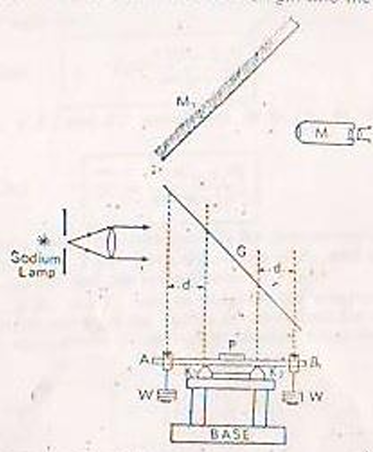
\includegraphics[width=0.5\textwidth]{draw.png}  % Replace with actual image filename
    \caption{Cornu's Method Experimental Setup}
\end{figure}
\vspace{1em}

\subsection{Mathematical Derivation \autocite{IITRCornuMethod}}
\noindent

The experimental beam AB is bent under the action of the loads \( W \) hanging at both ends. The bending moment \( G \) at all transverse sections of the central span is related to the longitudinal radius of curvature \( R_1 \) by:
\begin{equation}
G = \frac{YI}{R_1}
\end{equation}
where \( Y \) is the Young's modulus and \( I \) is the moment of inertia of the beam's cross-section:
\begin{equation}
I = \frac{1}{12}bt^3
\end{equation}
with \( b \) as the breadth and \( t \) the thickness of the beam.

If \( d \) is the distance between the knife-edge and the point of load application:
\begin{equation}
G = Wd
\end{equation}

Combining equations (7) and (9):
\begin{equation}
\frac{YI}{R_1} = Wd
\end{equation}

If the beam has an initial curvature \( R_0 \) due to its own weight, the equation becomes:
\begin{equation}
\frac{YI}{R_1} - \frac{YI}{R_0} = Wd
\end{equation}

For another load \( W' \), and radius \( R_1' \), analogously:
\begin{equation}
\frac{YI}{R_1'} - \frac{YI}{R_0} = W'd
\end{equation}

Subtracting these:
\begin{align}
YI &= \left( \frac{1}{R_1} - \frac{1}{R_1'} \right) = (W - W')d \notag \\
\Rightarrow Y &= \frac{(W - W')d}{I\left( \frac{1}{R_1} - \frac{1}{R_1'} \right)}
\end{align}

Substitute \( I \) from (8):
\begin{equation}
Y = \frac{12(W - W')d}{bt^3 \left( \frac{1}{R_1} - \frac{1}{R_1'} \right)}
\end{equation}

\subsection*{Determining \( R_1 \) from Fringes}

\begin{figure}[H]
    \centering
    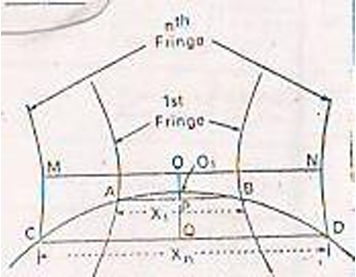
\includegraphics[width=0.6\textwidth]{geometry.png}
    \caption{Fringe Geometry for Determining Radii of Curvature}
\end{figure}

From fringe geometry:
\begin{align}
(2R_1 - O_1P) O_1P &= \left( \frac{X_1}{2} \right)^2 \notag \\
2R_1 \cdot O_1P &= \left( \frac{X_1}{2} \right)^2 \quad \text{(neglecting small } O_1P^2 \text{)}  \\
2R_1 \cdot O_1Q &= \left( \frac{X_n}{2} \right)^2
\end{align}

Subtracting (16) from (15), and using:
\begin{equation}
O_1Q - O_1P = \frac{(n-1)\lambda}{2}
\end{equation}
where \(R_x\) is the horizontal curvature and \(R_y\) is the vertical curvature. The bending moment induced by the applied loads is also related to the beam's geometry and material properties. By applying beam-bending theory, the second moment of area is calculated, and the relationship between the applied load, the beam's dimensions, and the curvature is established. This relationship allows for the calculation of Young's modulus \(E\) using the formula
yields:
\begin{align}
2R_1 \cdot \frac{(n-1)\lambda}{2} &= \frac{1}{4}(X_n^2 - X_1^2) \notag \\
\Rightarrow R_1 &= \frac{X_n^2 - X_1^2}{4\lambda(n-1)}
\end{align}

For another load \( W' \):
\begin{equation}
R_1' = \frac{X_n'^2 - X_1'^2}{4\lambda(n-1)}
\end{equation}

\subsection*{Poisson's Ratio from Transverse Fringes}

Similarly, using vertical fringe data:
\begin{equation}
R_y = \frac{Y_n^2 - Y_1^2}{4\lambda(n-1)}
\end{equation}

Poisson's ratio is:
\begin{equation}
\sigma = \frac{R_x}{R_y} = \frac{X_n^2 - X_1^2}{Y_n^2 - Y_1^2}
\end{equation}

\newpage
%%%%%%%%%%%%%%%%%%%%%%%%%%%%%%%%%%%%%%%%%
\phantomsection
\section{\centering METHODOLOGY}
\label{sec:METHODOLOGY}
% Methodology Part
\indent

\begin{figure}[H]
  \centering
  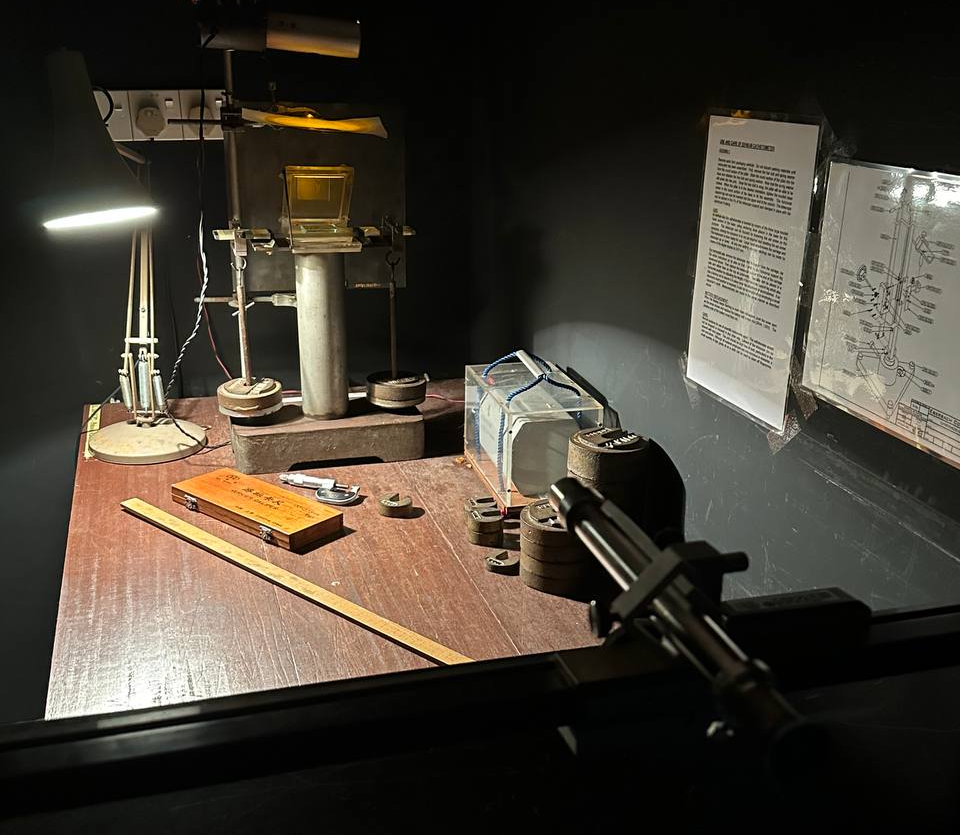
\includegraphics[width=0.75\textwidth]{image.png}
  \caption{Schematic of the Cornu interferometer and beam‑bending apparatus.}
  \label{fig:setup}
\end{figure}

A rectangular glass beam of measured breadth \(b\) and thickness \(d\) was carefully placed on two knife-edge supports such that known masses \(m\) could be suspended at equal distances \(a\) from these supports. The beam's dimensions were determined with vernier calipers and a micrometer screw gauge, ensuring minimal dimensional uncertainty.\\

A flat square glass plate was gently positioned at the beam's center, forming a narrow air gap between the beam's upper surface and the plate. This setup was illuminated by a sodium lamp of wavelength \(\lambda \approx 589.3\,\mathrm{nm}\), and a \(45^\circ\) mirror directed the reflected interference fringes into a stage telescope equipped with \(x\)- and \(y\)-direction micrometers.\\

After focusing the telescope to obtain clear fringes, the fringes were measured first along the horizontal axis and then along the vertical axis by recording pairs of positions \((x',x)\) or \((y',y)\) for each fringe, where each fringe was assigned an integer index \(n\). By subtracting these pairs, the displacements \(\Delta X_n = x - x'\) and \(\Delta Y_n = y - y'\) were found, squared to obtain \(\Delta X_n^2\) and \(\Delta Y_n^2\), and subsequently plotted as functions of \(n\).\\

Linear regressions of these plots determined the slopes corresponding to \(4\,\lambda\,R_x\) and \(4\,\lambda\,R_y\), from which the radii of curvature \(R_x\) and \(R_y\) were calculated. Poisson's ratio was evaluated as \(\sigma = R_x / R_y\), taking each load's horizontal and vertical radii into account.\\

In order to find Young's modulus \(E\), the experiment focused on the primary bending of the beam (horizontal displacement), employing the standard bending formula 
\begin{equation}
E = \frac{12\,m\,g\,a\,R_x}{b\,d^3}.
\end{equation}
where \(R_x\) is the horizontal curvature and \(R_y\) is the vertical curvature. The bending moment induced by the applied loads is also related to the beam's geometry and material properties. By applying beam-bending theory, the second moment of area is calculated, and the relationship between the applied load, the beam's dimensions, and the curvature is established. This relationship allows for the calculation of Young's modulus \(E\) using the formula
The gravitational acceleration \(g\) was taken as \(9.81\,\mathrm{m\,s}^{-2}\), and each measurement's uncertainty, including those in \(b\), \(d\), \(a\), and the slope-derived \(R_x\) and \(R_y\), was used in an error-propagation calculation.\\

From these combined uncertainties, the final values for \(\sigma\) and \(E\) were obtained, providing a reliable characterization of the glass beam's elastic properties.

\newpage
%%%%%%%%%%%%%%%%%%%%%%%%%%%%%%%%%%%%%%%%%%
\phantomsection
\section{\centering DATA ANALYSIS}
\label{sec:DATA ANALYSIS}
% Content for the DATA ANALYSIS section goes here.
\textbf{All data, calculation and programming python code of the experments are attached in the Appendices.}\\

\subsection{Fringe Pattern Observations}
\label{subsec:FRINGE PATTERN}
\noindent 

The following figures display the interference fringe pattern observed on the glass beam when loads is applied to each side. The clearly defined fringes indicate proper alignment of the optical setup and serve as the foundation for determining the beam's radii of curvature through subsequent analysis.\\

% Figurewith interference fringes
\begin{figure}[H]
  \centering
  % Replace "interference_fringes_1kg.jpg" with the actual filename of your image
  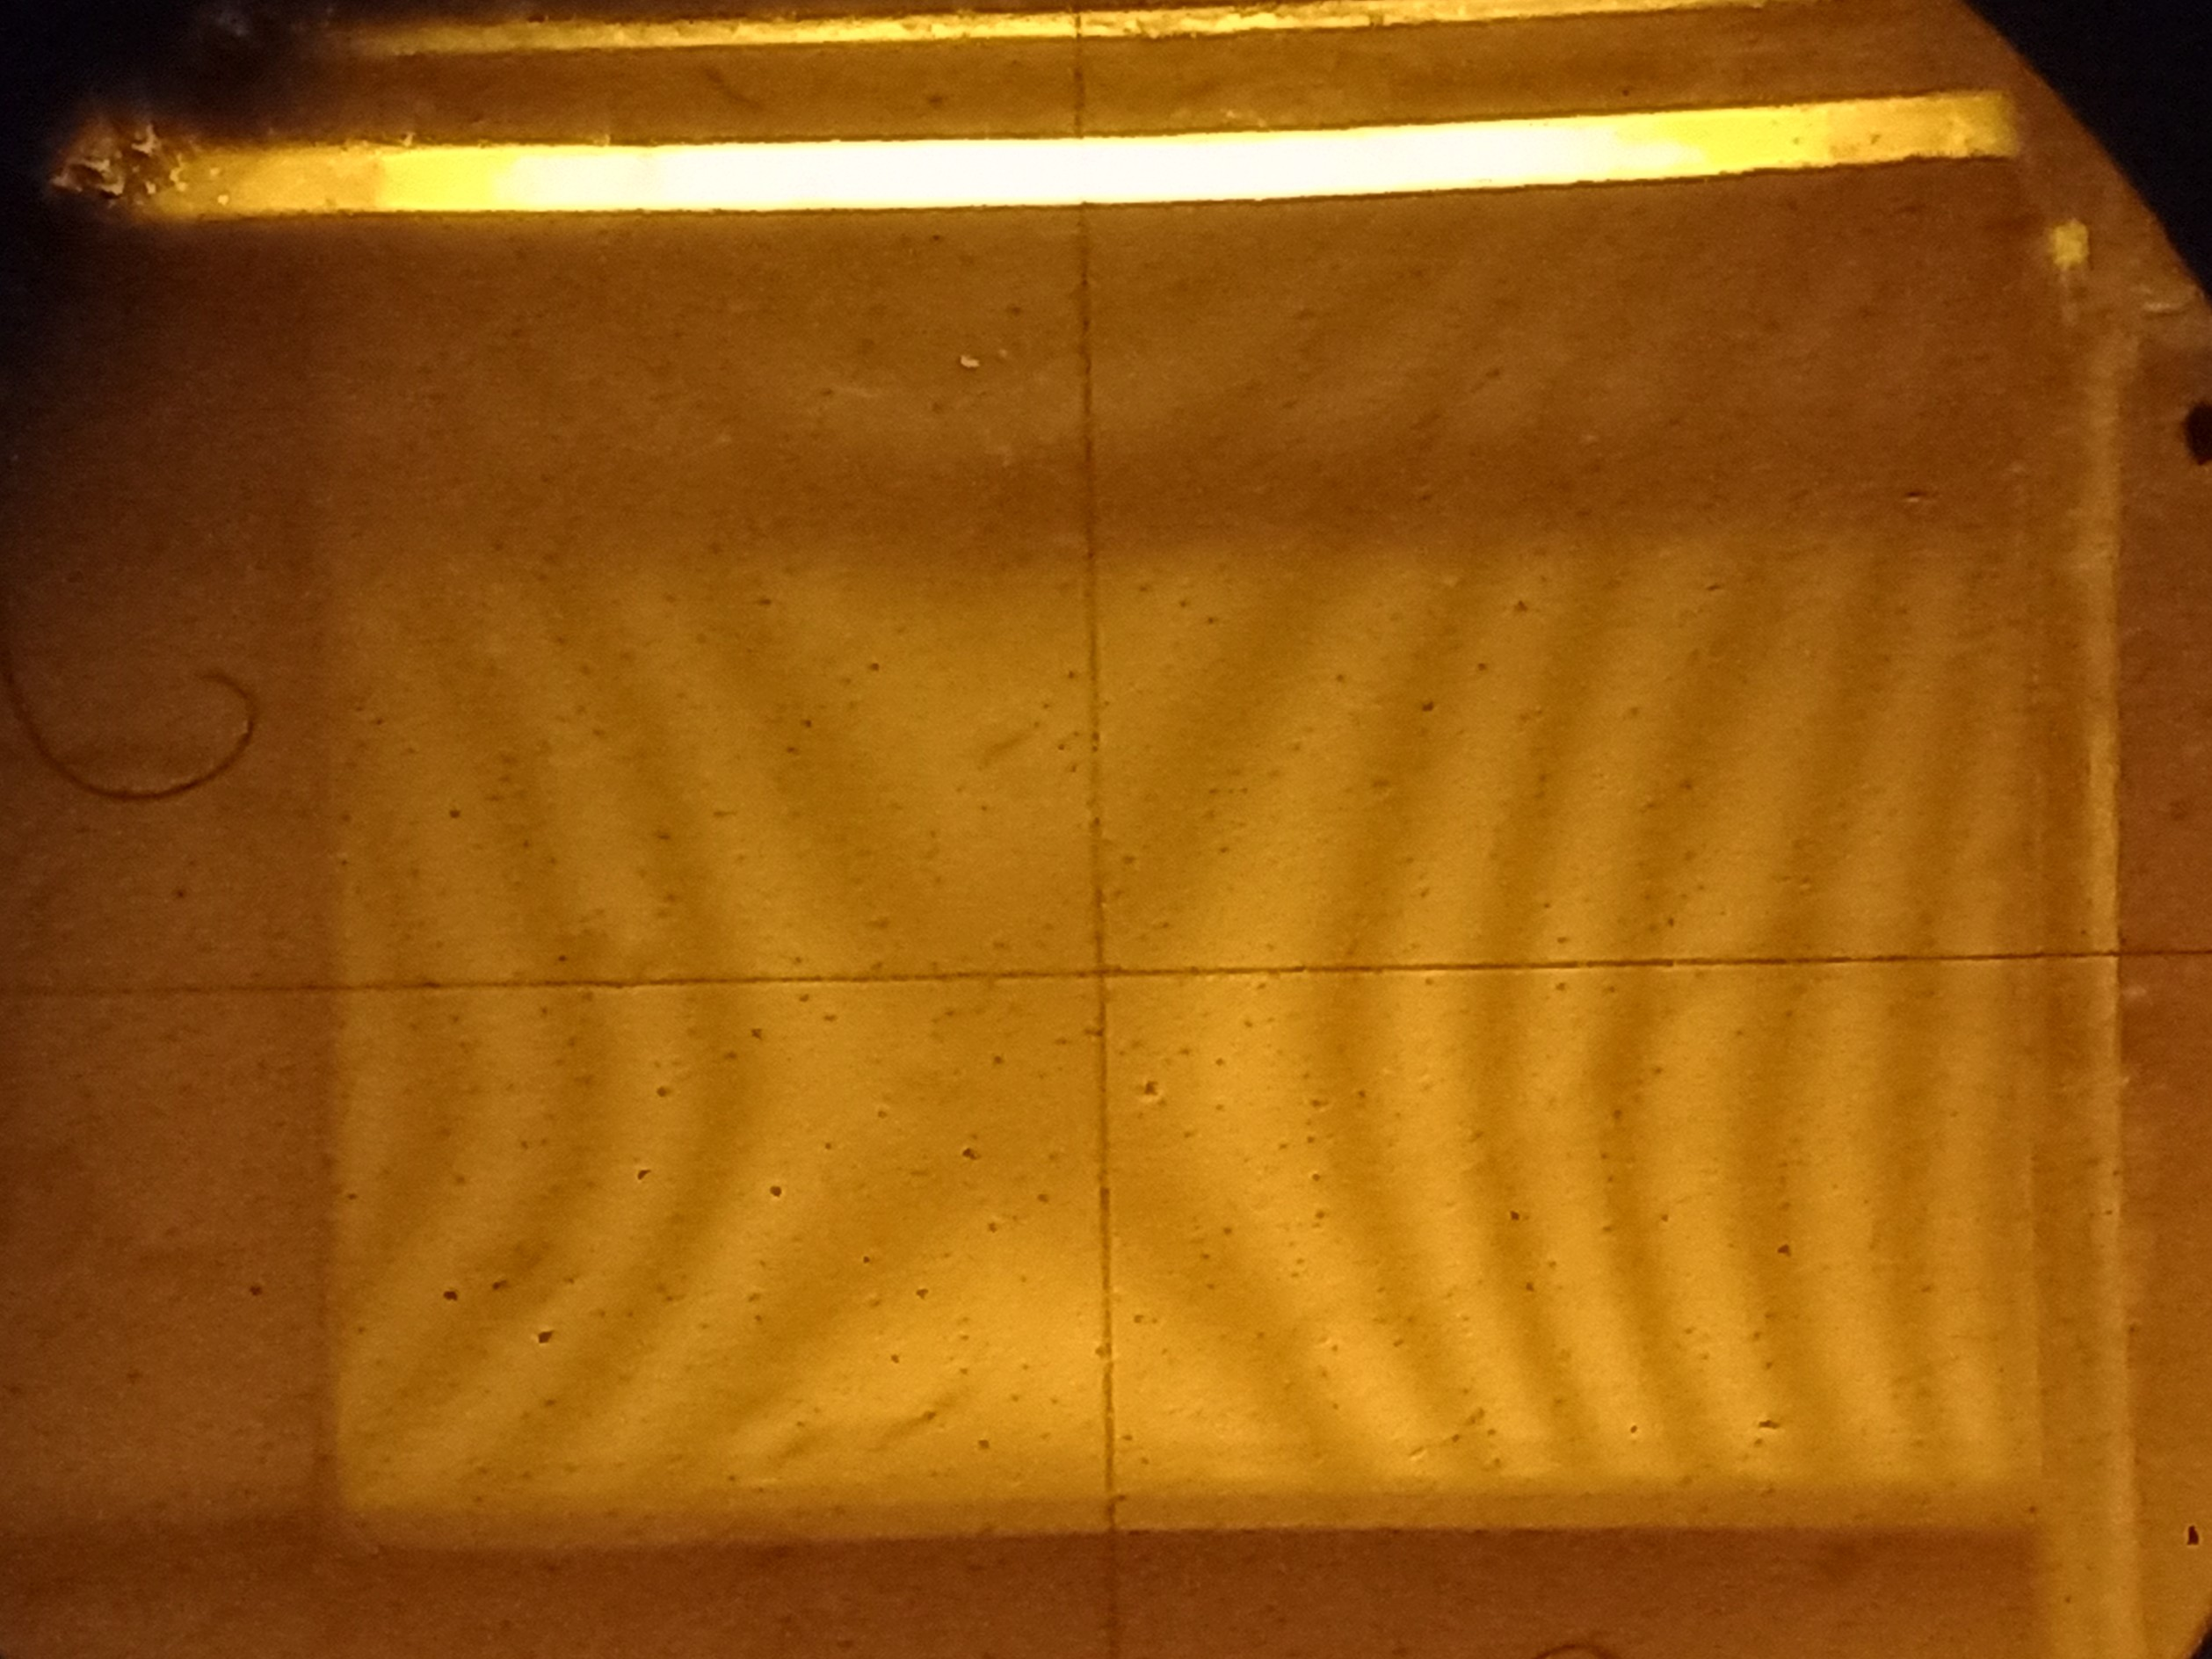
\includegraphics[width=0.6\textwidth]{1.jpg}
  \caption{Interference fringes observed for the glass beam, loaded with 1\,kg on each side. 
  The crossed lines indicate the telescope's reticle used to align and measure the fringe positions.}
  \label{fig:fringes_1kg}
\end{figure}

\begin{figure}[H]
  \centering
  % First row: left subfigure (3 kg)
  \begin{subfigure}[b]{0.45\textwidth}
    \centering
    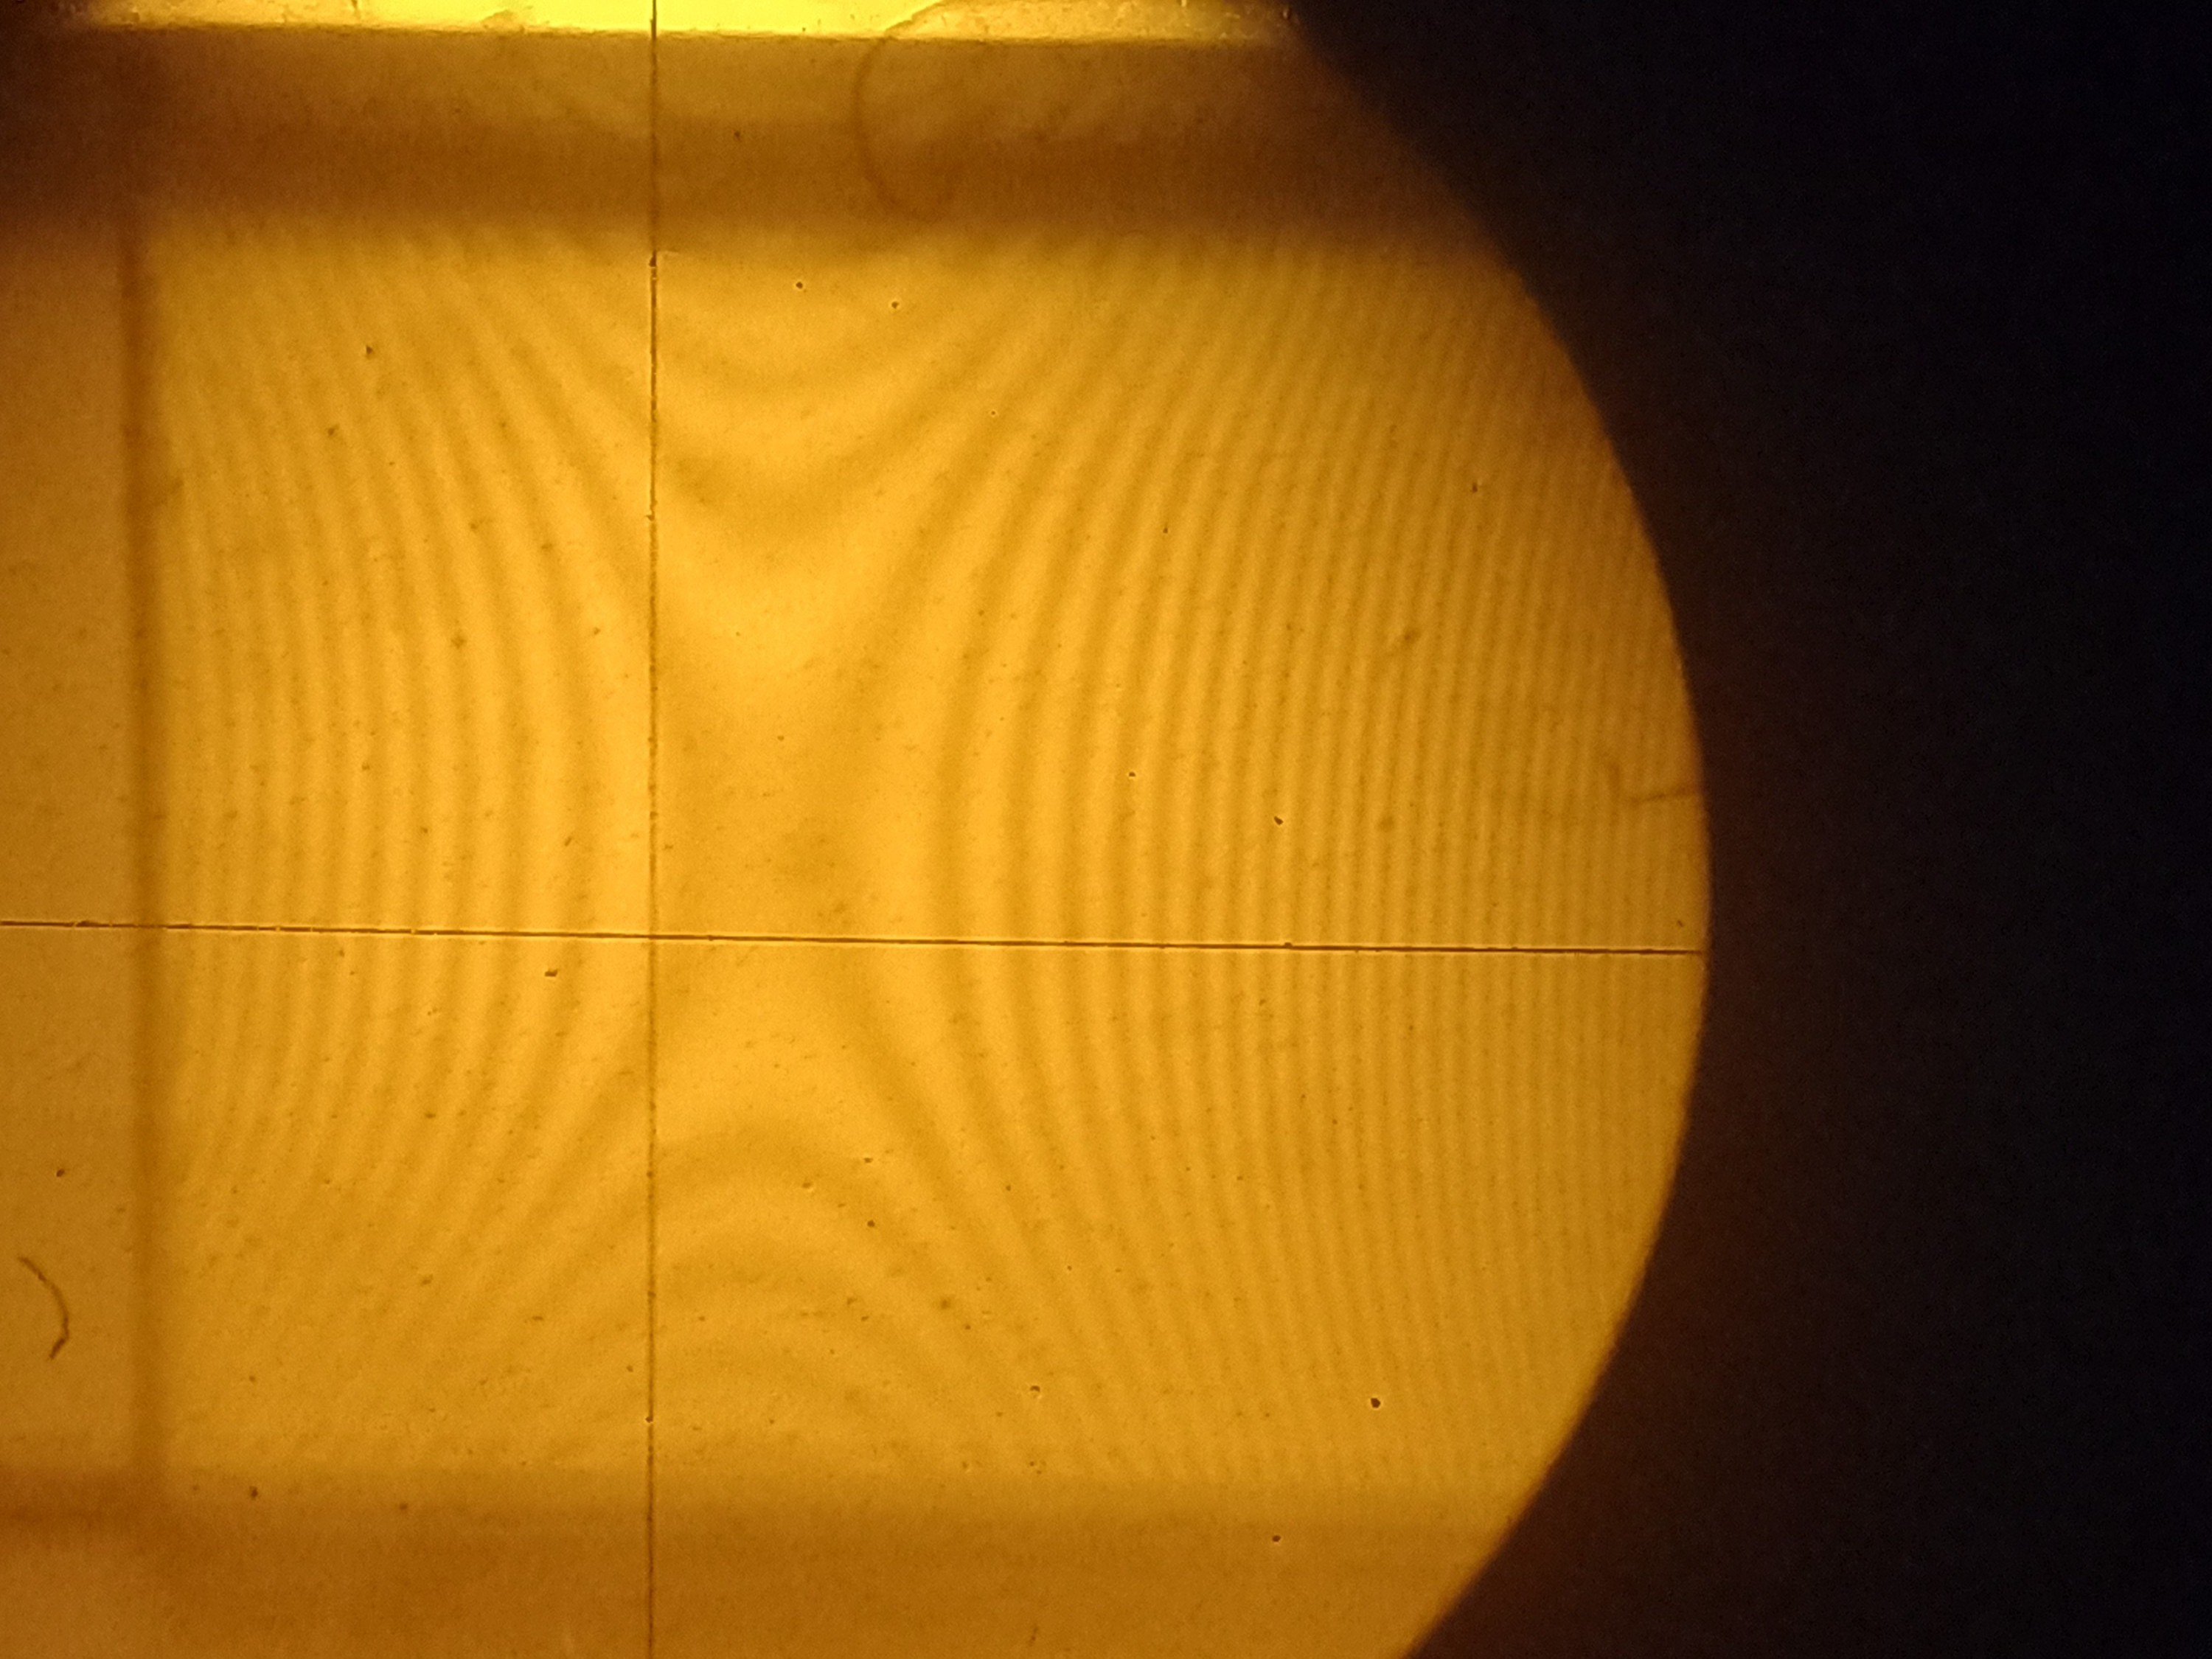
\includegraphics[width=\textwidth]{3.jpg}
    \caption{Interference fringes for 3\,kg on each side.}
    \label{fig:fringes_3kg}
  \end{subfigure}
  \hfill
  % First row: right subfigure (4 kg)
  \begin{subfigure}[b]{0.45\textwidth}
    \centering
    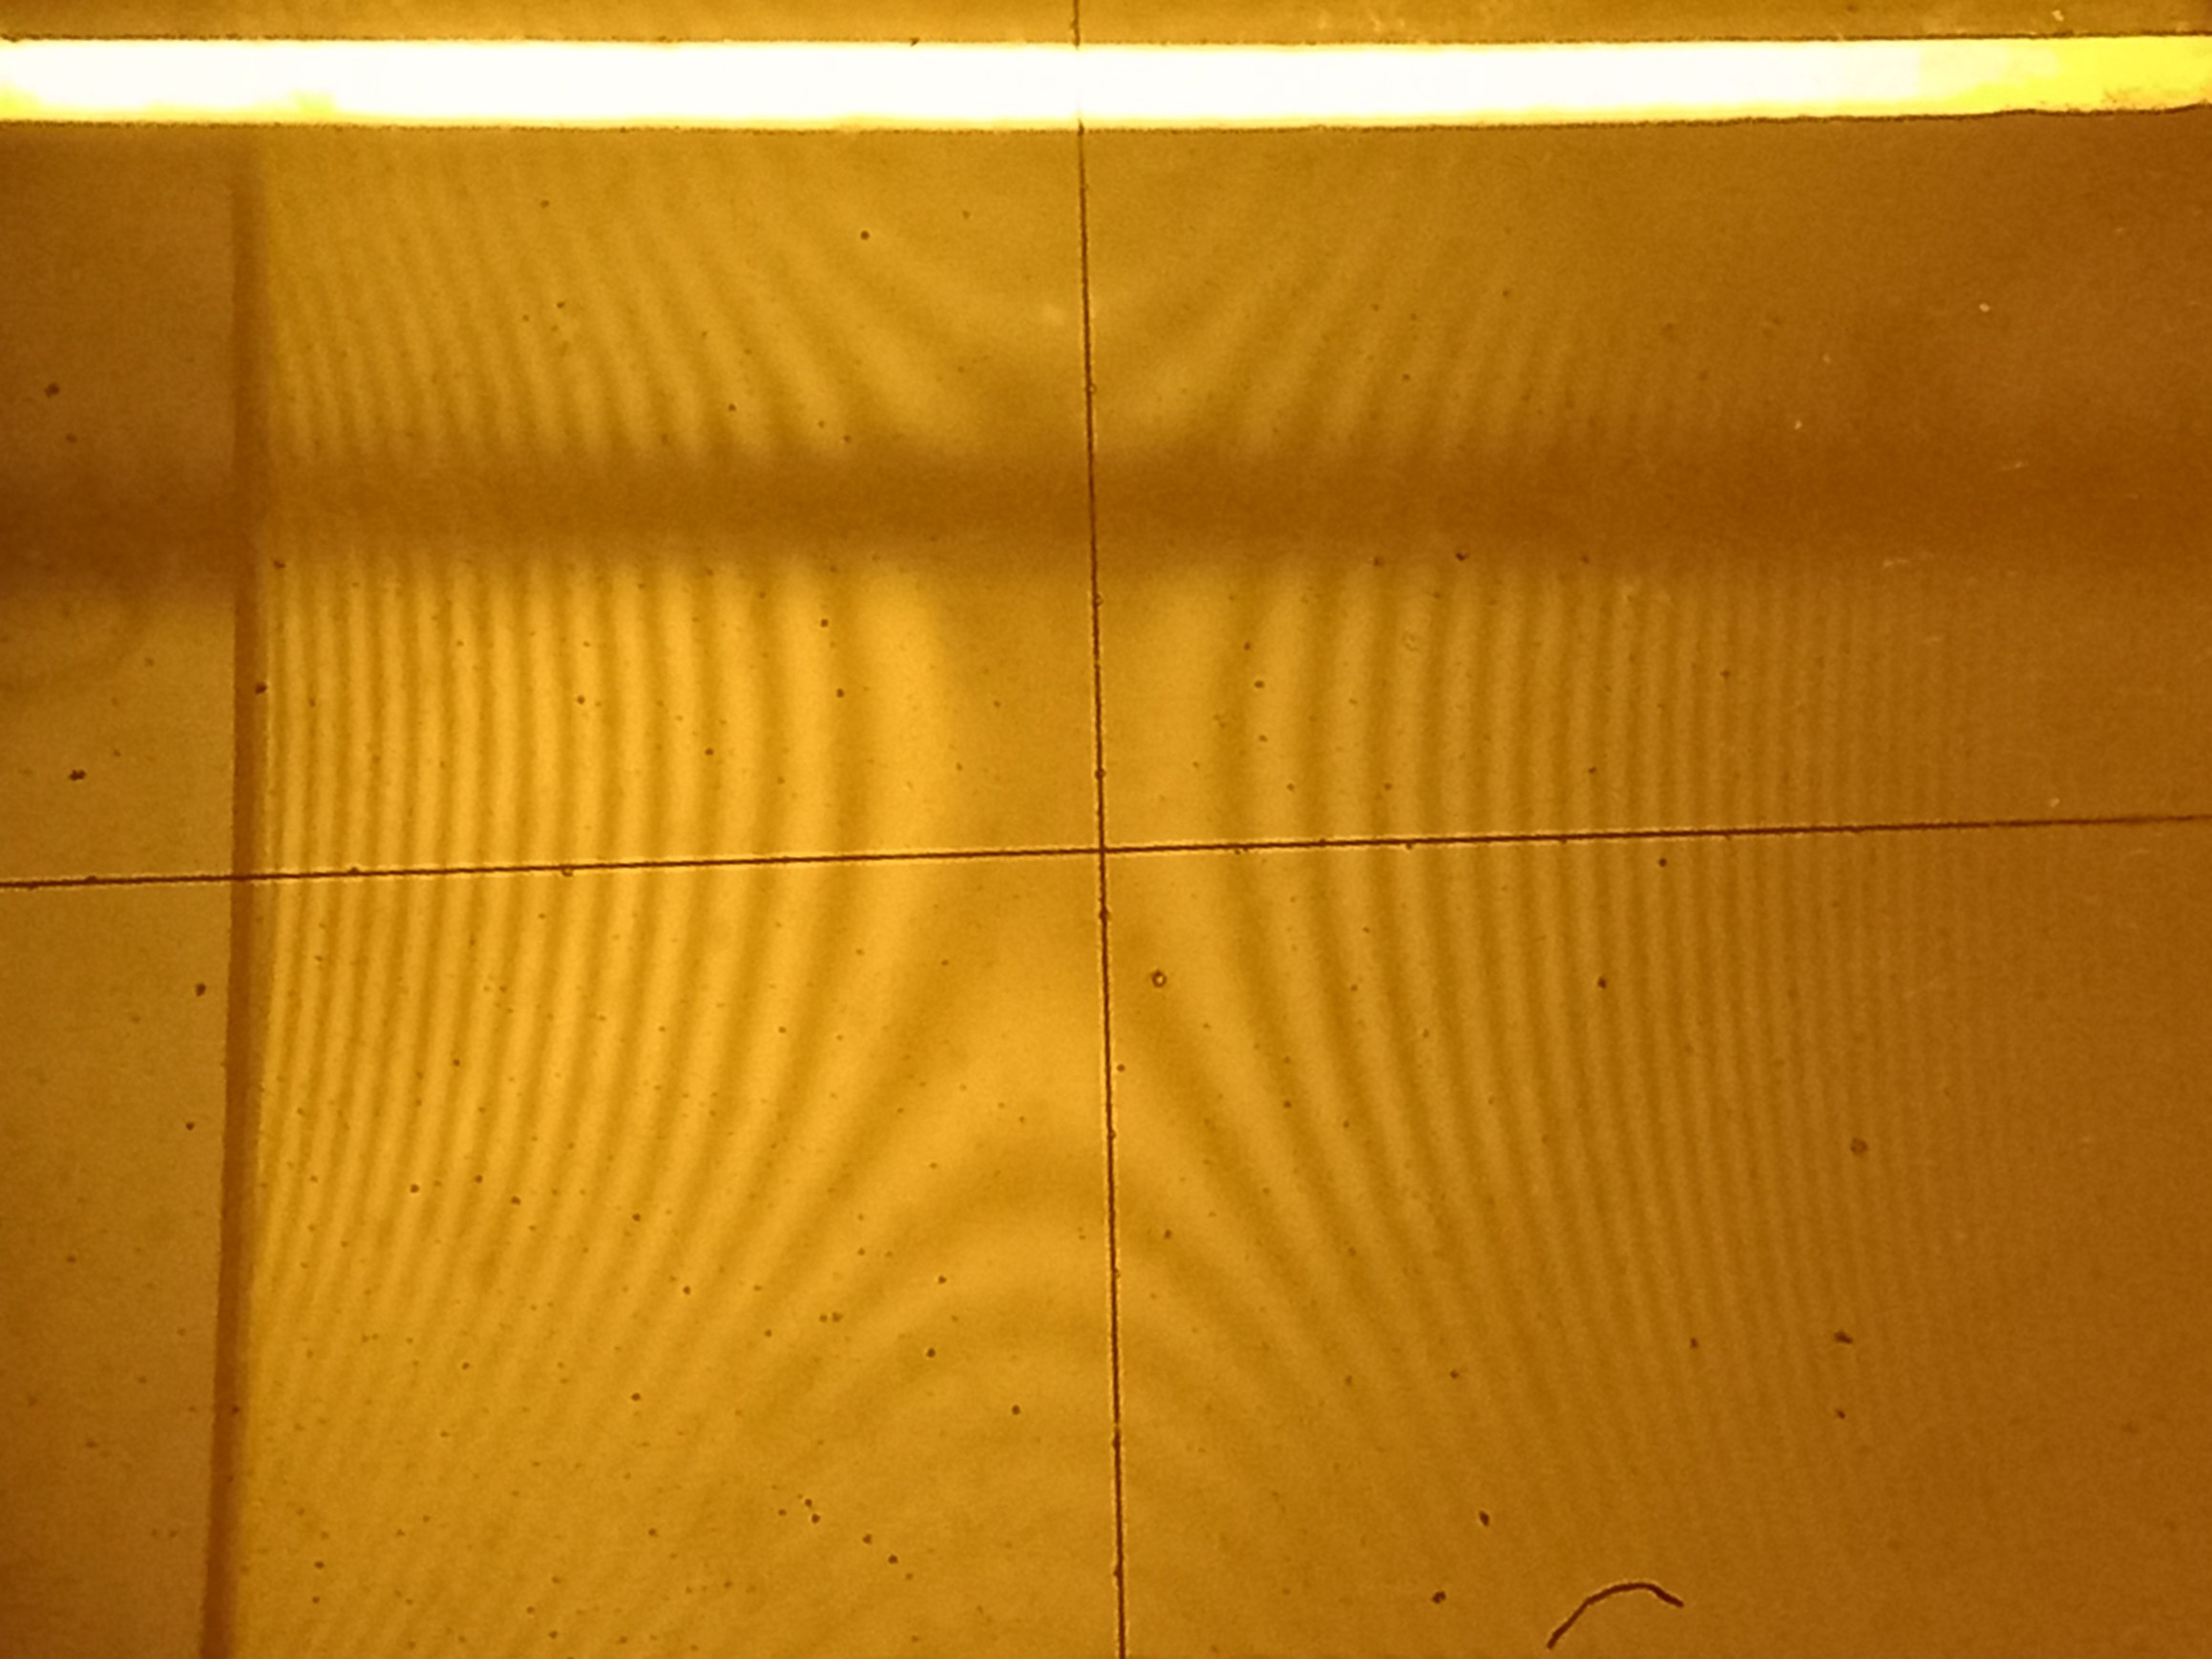
\includegraphics[width=\textwidth]{4.jpg}
    \caption{Interference fringes for 4\,kg on each side.}
    \label{fig:fringes_4kg}
  \end{subfigure}
  
  \vspace{1em} % Adjust vertical space between rows as needed
  
  % Second row: left subfigure (5 kg)
  \begin{subfigure}[b]{0.45\textwidth}
    \centering
    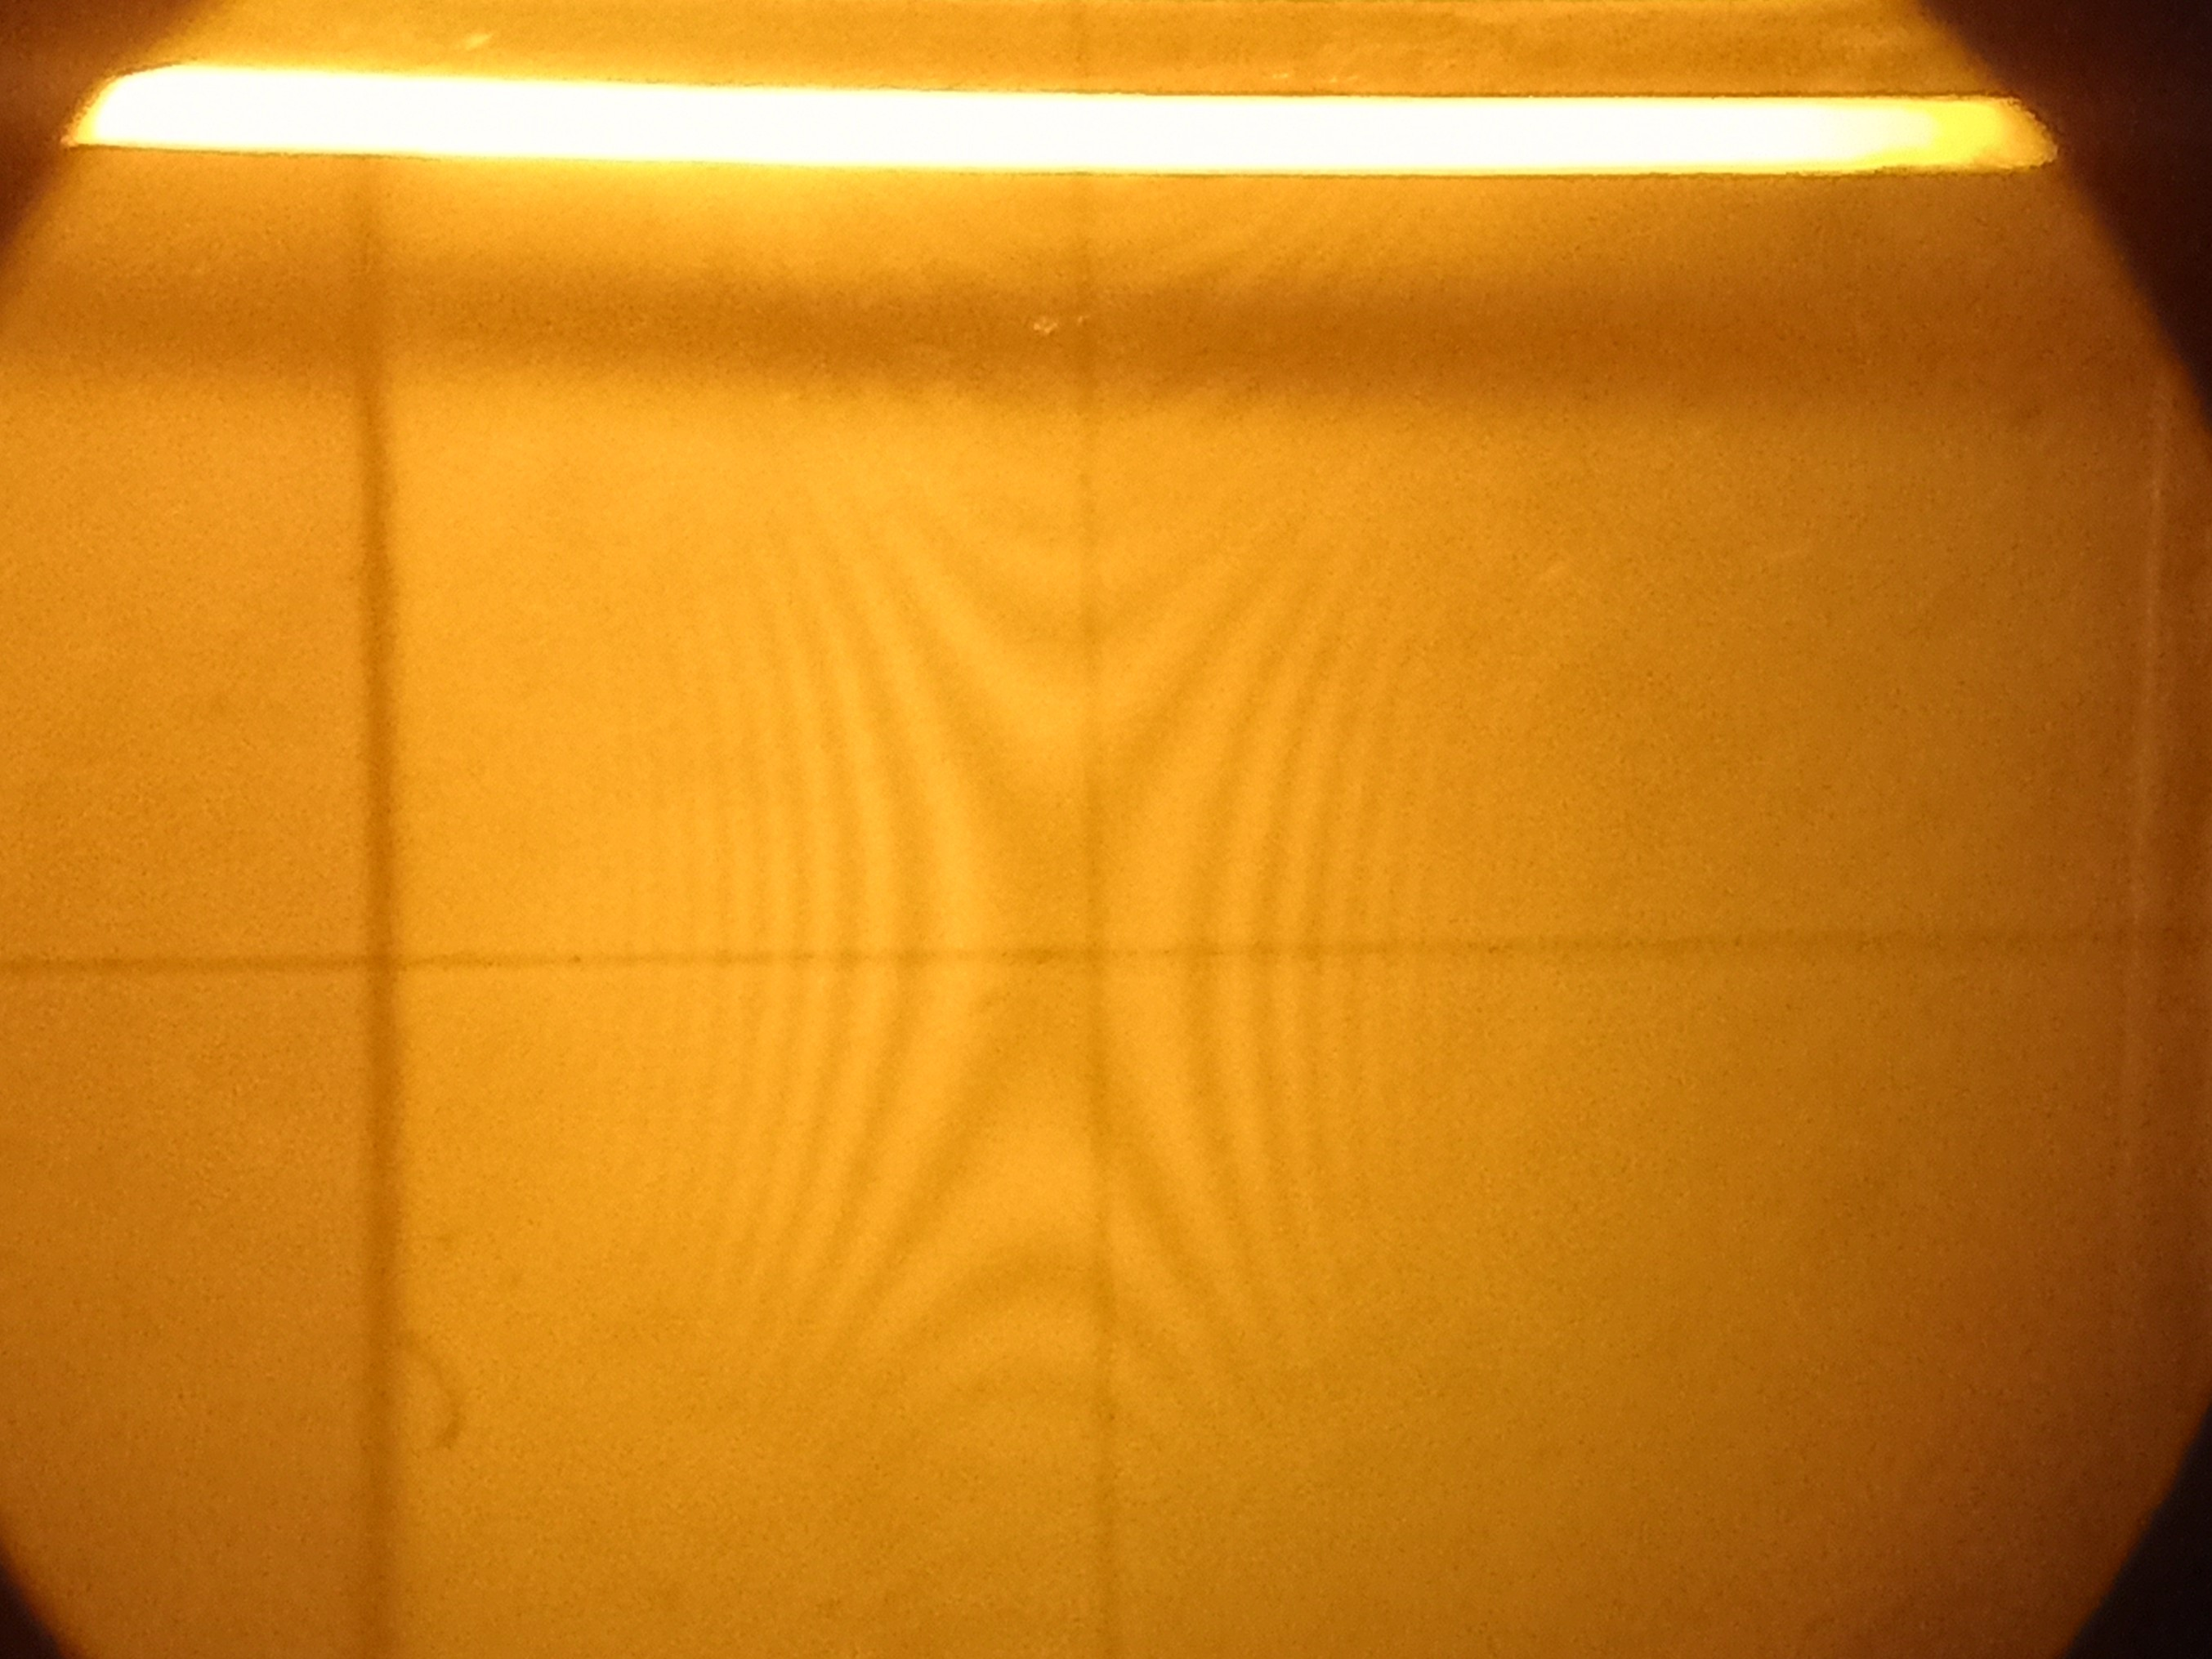
\includegraphics[width=\textwidth]{5.jpg}
    \caption{Interference fringes for 5\,kg on each side.}
    \label{fig:fringes_5kg}
  \end{subfigure}
  \hfill
  % Second row: right subfigure (6 kg)
  \begin{subfigure}[b]{0.45\textwidth}
    \centering
    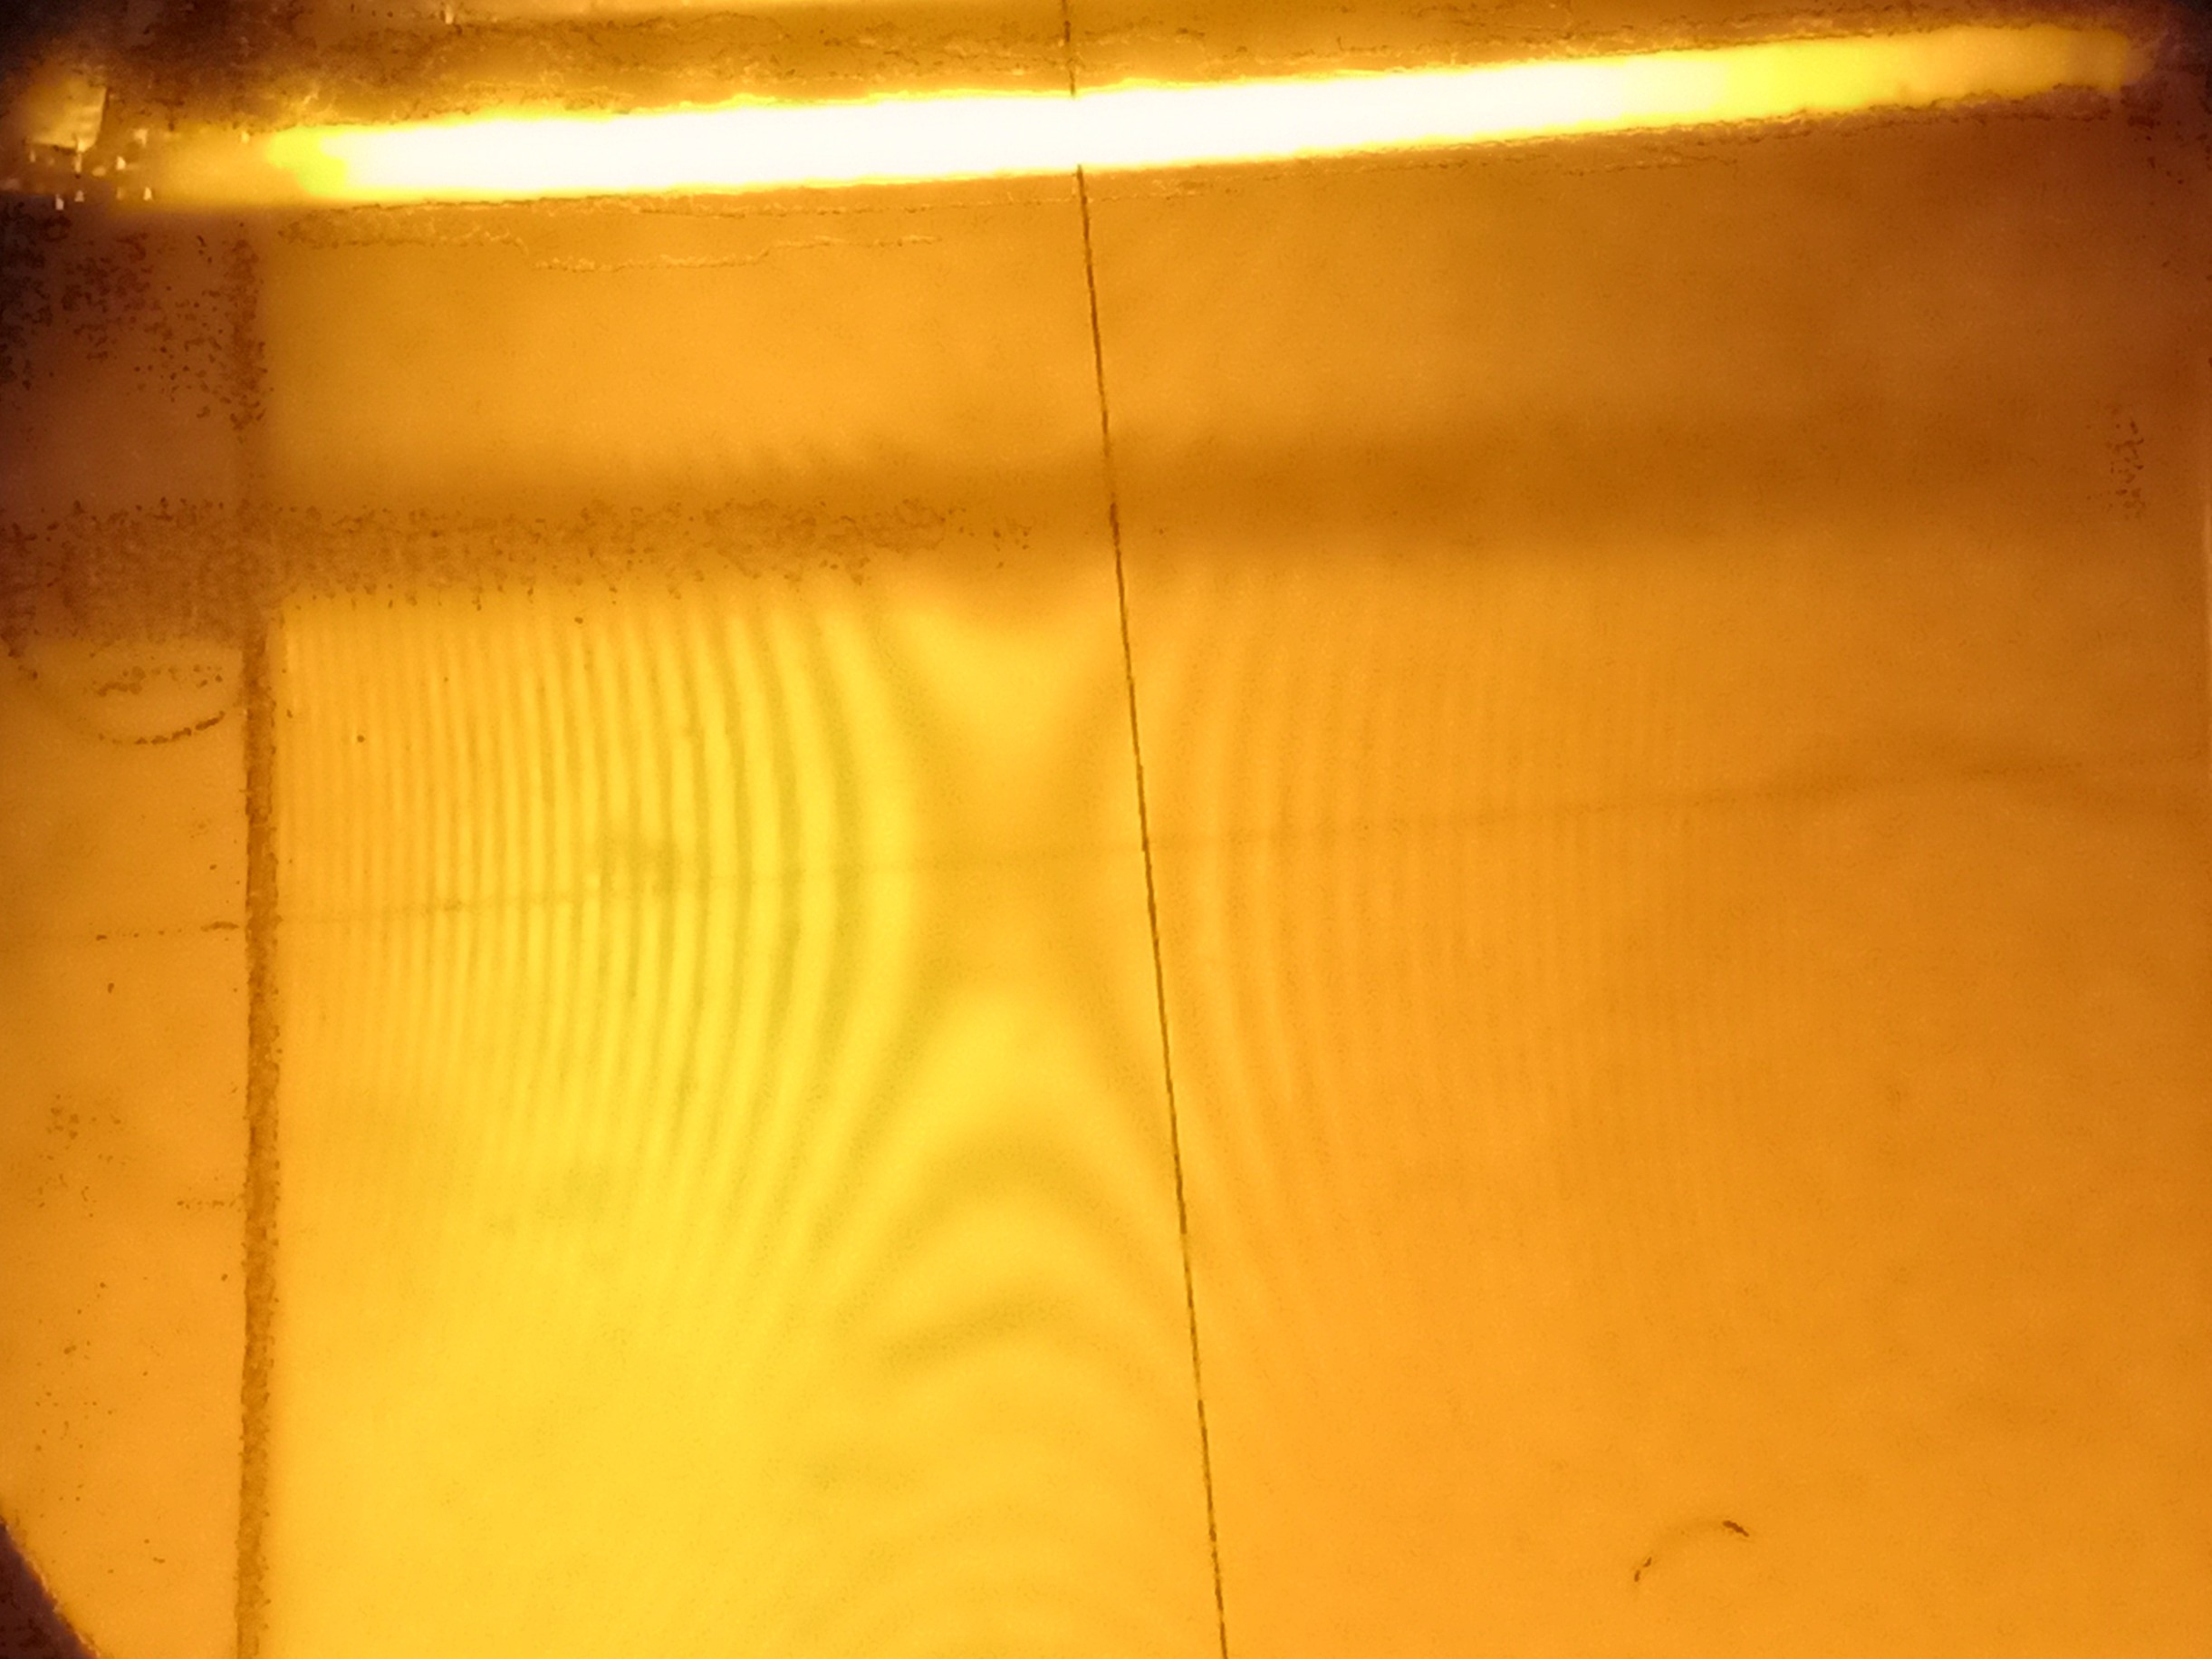
\includegraphics[width=\textwidth]{6.jpg}
    \caption{Interference fringes for 6\,kg on each side.}
    \label{fig:fringes_6kg}
  \end{subfigure}
  
  \caption{Interference fringes observed for the glass beam under various loadings. The crossed lines indicate the telescope's reticle used to align and measure the fringe positions.}
  \label{fig:fringes_combined}
\end{figure}

\subsection{Experimental Measurements and Tabulated Data}
\label{subsec:DATA}
\noindent

The experimental measurements were meticulously recorded and are presented in the following tables. The data comprises fringe measurements for a rectangular glass beam subjected to various loading conditions. Specifically, measurements were obtained for loads of 1\,kg, 3\,kg, 4\,kg, 5\,kg, and 6\,kg, with each load yielding data in two distinct orientations: horizontal and vertical.\\

For each mass and orientation, the tables list the fringe index \(n\), the micrometer readings from both sides of the central fringe (denoted \(x'\) and \(x\) in the horizontal orientation, or \(y'\) and \(y\) in the vertical orientation), the computed difference (\(X = x - x'\) or \(Y = y - y'\)), the squared difference (\(X^2\) or \(Y^2\)), and the associated uncertainty (\(\delta X^2\) or \(\delta Y^2\)). These computed quantities are critical for determining the radii of curvature of the beam under each load, which are subsequently used to extract the elastic properties of the glass.\\

In total, there are five tables: five for the horizontal data and vertical data. Each pair of horizontal and vertical tables for a given load enables a comprehensive analysis of the interference fringe pattern, thereby providing a robust basis for calculating both Poisson's ratio and Young's modulus.\\ 


% =============================================================================
% 1 kg — HORIZONTAL (left) and VERTICAL (right)
% =============================================================================
\begin{table}[H]
  \centering
  \caption{1 kg — HORIZONTAL (left) and VERTICAL (right)}\label{tab:1kg-hv}
  \begin{subtable}[t]{0.47\linewidth}
    \centering
    \caption*{\textbf{HORIZONTAL}}\label{tab:1kg-h}
    \begin{tabular}{cccc}
      \toprule
      $n$ & $X$ (mm) & $X^2$ (mm$^2$) & $\delta X^2$ (mm$^2$)\\
      \midrule
       4 & 37.41 & 1399.51 & 1.06\\
       3 & 28.46 &  809.97 & 0.80\\
       2 & 19.58 &  383.38 & 0.55\\
       1 &  7.95 &   63.20 & 0.22\\
      \bottomrule
    \end{tabular}
  \end{subtable}
  \hfill
  \begin{subtable}[t]{0.47\linewidth}
    \centering
    \caption*{\textbf{VERTICAL}}\label{tab:1kg-v}
    \begin{tabular}{cccc}
      \toprule
      $n$ & $Y$ (mm) & $Y^2$ (mm$^2$) & $\delta Y^2$ (mm$^2$)\\
      \midrule
       2 & 31.34 &  982.20 & 0.89\\
       1 & 18.21 &  331.60 & 0.52\\
      \bottomrule
    \end{tabular}
  \end{subtable}
\end{table}

% =============================================================================
% 3 kg — HORIZONTAL (left) and VERTICAL (right)
% =============================================================================
\begin{table}[H]
  \centering
  \caption{3 kg — HORIZONTAL (left) and VERTICAL (right)}\label{tab:3kg-hv}
  \begin{subtable}[t]{0.47\linewidth}
    \centering
    \caption*{\textbf{HORIZONTAL}}\label{tab:3kg-h}
    \begin{tabular}{cccc}
      \toprule
      $n$ & $X$ (mm) & $X^2$ (mm$^2$) & $\delta X^2$ (mm$^2$)\\
      \midrule
       6 & 25.34 &  642.12 & 0.72\\
       5 & 21.77 &  473.93 & 0.62\\
       4 & 18.73 &  350.81 & 0.53\\
       3 & 15.29 &  233.78 & 0.43\\
       2 & 11.11 &  123.43 & 0.31\\
       1 &  4.38 &   19.18 & 0.12\\
      \bottomrule
    \end{tabular}
  \end{subtable}
  \hfill
  \begin{subtable}[t]{0.47\linewidth}
    \centering
    \caption*{\textbf{VERTICAL}}\label{tab:3kg-v}
    \begin{tabular}{cccc}
      \toprule
      $n$ & $Y$ (mm) & $Y^2$ (mm$^2$) & $\delta Y^2$ (mm$^2$)\\
      \midrule
       4 & 35.90 & 1288.81 & 1.02\\
       3 & 31.74 & 1007.43 & 0.90\\
       2 & 26.91 &  724.15 & 0.76\\
       1 & 19.50 &  380.25 & 0.55\\
      \bottomrule
    \end{tabular}
  \end{subtable}
\end{table}

% =============================================================================
% 4 kg — HORIZONTAL (left) and VERTICAL (right)
% =============================================================================
\begin{table}[H]
  \centering
  \caption{4 kg — HORIZONTAL (left) and VERTICAL (right)}\label{tab:4kg-hv}
  \begin{subtable}[t]{0.47\linewidth}
    \centering
    \caption*{\textbf{HORIZONTAL}}\label{tab:4kg-h}
    \begin{tabular}{cccc}
      \toprule
      $n$ & $X$ (mm) & $X^2$ (mm$^2$) & $\delta X^2$ (mm$^2$)\\
      \midrule
       6 & 21.16 & 447.75 & 0.60\\
       5 & 18.85 & 355.32 & 0.53\\
       4 & 16.67 & 277.89 & 0.47\\
       3 & 13.13 & 172.40 & 0.37\\
       2 &  9.54 &  91.01 & 0.27\\
       1 &  3.69 &  13.62 & 0.10\\
      \bottomrule
    \end{tabular}
  \end{subtable}
  \hfill
  \begin{subtable}[t]{0.47\linewidth}
    \centering
    \caption*{\textbf{VERTICAL}}\label{tab:4kg-v}
    \begin{tabular}{cccc}
      \toprule
      $n$ & $Y$ (mm) & $Y^2$ (mm$^2$) & $\delta Y^2$ (mm$^2$)\\
      \midrule
       6 & 36.63 & 1341.76 & 1.04\\
       5 & 34.55 & 1193.70 & 0.98\\
       4 & 29.95 &  897.00 & 0.85\\
       3 & 24.95 &  622.50 & 0.71\\
       2 & 18.30 &  334.89 & 0.52\\
       1 &  3.15 &    9.92 & 0.09\\
      \bottomrule
    \end{tabular}
  \end{subtable}
\end{table}

% =============================================================================
% 5 kg — HORIZONTAL (left) and VERTICAL (right)
% =============================================================================
\begin{table}[H]
  \centering
  \caption{5 kg — HORIZONTAL (left) and VERTICAL (right)}\label{tab:5kg-hv}
  \begin{subtable}[t]{0.47\linewidth}
    \centering
    \caption*{\textbf{HORIZONTAL}}\label{tab:5kg-h}
    \begin{tabular}{cccc}
      \toprule
      $n$ & $X$ (mm) & $X^2$ (mm$^2$) & $\delta X^2$ (mm$^2$)\\
      \midrule
       6 & 18.65 & 347.82 & 0.53\\
       5 & 16.56 & 274.23 & 0.47\\
       4 & 14.10 & 198.81 & 0.40\\
       3 & 11.14 & 124.10 & 0.32\\
       2 &  7.32 &  53.58 & 0.21\\
       1 &  1.35 &   1.82 & 0.04\\
      \bottomrule
    \end{tabular}
  \end{subtable}
  \hfill
  \begin{subtable}[t]{0.47\linewidth}
    \centering
    \caption*{\textbf{VERTICAL}}\label{tab:5kg-v}
    \begin{tabular}{cccc}
      \toprule
      $n$ & $Y$ (mm) & $Y^2$ (mm$^2$) & $\delta Y^2$ (mm$^2$)\\
      \midrule
       6 & 35.33 & 1248.21 & 1.00\\
       5 & 31.72 & 1006.16 & 0.90\\
       4 & 27.85 &  775.62 & 0.79\\
       3 & 23.60 &  556.96 & 0.67\\
       2 & 17.78 &  316.13 & 0.50\\
       1 &  6.49 &   42.12 & 0.18\\
      \bottomrule
    \end{tabular}
  \end{subtable}
\end{table}

% =============================================================================
% 6 kg — HORIZONTAL (left) and VERTICAL (right)
% =============================================================================
\begin{table}[H]
  \centering
  \caption{6 kg — HORIZONTAL (left) and VERTICAL (right)}\label{tab:6kg-hv}
  \begin{subtable}[t]{0.47\linewidth}
    \centering
    \caption*{\textbf{HORIZONTAL}}\label{tab:6kg-h}
    \begin{tabular}{cccc}
      \toprule
      $n$ & $X$ (mm) & $X^2$ (mm$^2$) & $\delta X^2$ (mm$^2$)\\
      \midrule
       6 & 17.94 & 321.84 & 0.51\\
       5 & 16.23 & 263.41 & 0.46\\
       4 & 13.97 & 195.16 & 0.40\\
       3 & 11.55 & 133.40 & 0.33\\
       2 &  8.68 &  75.34 & 0.25\\
       1 &  3.38 &  11.42 & 0.10\\
      \bottomrule
    \end{tabular}
  \end{subtable}
  \hfill
  \begin{subtable}[t]{0.47\linewidth}
    \centering
    \caption*{\textbf{VERTICAL}}\label{tab:6kg-v}
    \begin{tabular}{cccc}
      \toprule
      $n$ & $Y$ (mm) & $Y^2$ (mm$^2$) & $\delta Y^2$ (mm$^2$)\\
      \midrule
       6 & 35.17 & 1236.93 & 0.99\\
       5 & 30.77 &  946.79 & 0.87\\
       4 & 27.72 &  768.40 & 0.78\\
       3 & 23.51 &  552.72 & 0.66\\
       2 & 19.14 &  366.34 & 0.54\\
       1 & 11.38 &  129.50 & 0.32\\
      \bottomrule
    \end{tabular}
  \end{subtable}
\end{table}

The data presented in the tables clearly illustrates the expected trend between the fringe order \(n\) and the computed squared differences (\(X^2\) or \(Y^2\)). As the fringe index increases, both the absolute difference in the micrometer readings and hence their squares also increase, in accordance with the theoretical prediction that
\begin{equation}
X_n^2 = 4\,\lambda\,R_x\,n - c_x.
\end{equation}
where \(R_x\) is the horizontal curvature and \(R_y\) is the vertical curvature. The bending moment induced by the applied loads is also related to the beam's geometry and material properties. By applying beam-bending theory, the second moment of area is calculated, and the relationship between the applied load, the beam's dimensions, and the curvature is established. This relationship allows for the calculation of Young's modulus \(E\) using the formula
This linear relationship implies that higher fringe numbers correspond to larger path differences in the interference pattern, which is directly related to the bending curvature of the beam.\\

Based on the data in ~\autoref{tab:1kg-hv}--\autoref{tab:6kg-hv}, the squared deflections \(X^2\) and \(Y^2\) scale monotonically with the index \(n\) for each applied load. For instance, in the 1 kg horizontal measurements, \(X^2\) increases from 63.20\,mm\(^2\) at \(n=1\) to 1399.51\,mm\(^2\) at \(n=4\), while the corresponding vertical values grow from 331.60\,mm\(^2\) to 982.20\,mm\(^2\). The 3 kg dataset shows a rise in \(X^2\) from 19.18\,mm\(^2\) to 642.12\,mm\(^2\) and in \(Y^2\) from 380.25\,mm\(^2\) to 1288.81\,mm\(^2\); similar linear trends are evident for 4 kg, 5 kg, and 6 kg. These consistent linear relationships confirm our beam model, in which the applied load alters the slope of the \(X^2\)–\(n\) (or \(Y^2\)–\(n\)) line and thus the inferred radius of curvature.\\


Minor deviations from perfect linearity, seen as slight fluctuations in the squared fringe differences and their uncertainties (\(\delta X^2\) and \(\delta Y^2\)), suggest the influence of practical experimental factors. These include imperfections in the flatness of the glass surfaces, misalignments in the optical setup, and ambient vibrations during measurements. As \(n\) increases, any small inconsistencies in measurement may become amplified due to the larger fringe separations, which in turn affect the overall slope determination.\\

Ultimately, the observed changes in \(X^2\) and \(Y^2\) with respect to \(n\) not only confirm the linear dependency predicted by the theoretical model but also provide a reliable basis for calculating the radii of curvature. This is essential for further determining the elastic properties, such as Poisson's ratio and Young's modulus, of the glass beam. The robust and systematic behavior of the data with respect to the fringe order underscores the validity of using interference fringe analysis in material characterization.\\

\subsection{Linear Regression of Squared Displacements}
\label{subsec:LINEAR REGRESSION}
\indent 

The following figures display the linear regression plots of the squared fringe separations versus the fringe order for both horizontal and vertical orientations across different loads. These graphs provide a visual confirmation of the expected linear relationships derived from Cornu's method, where the slope of each line is directly proportional to the corresponding radius of curvature. By examining these plots, one can clearly observe how increasing the fringe order leads to larger squared displacements, thereby validating the theoretical model and facilitating the extraction of elastic properties.\\

% Graph Plots
\begin{figure}[H]
  \centering
  % First row: left subfigure (1 kg -- X^2 vs. n)
  \begin{subfigure}[b]{0.45\textwidth}
    \centering
    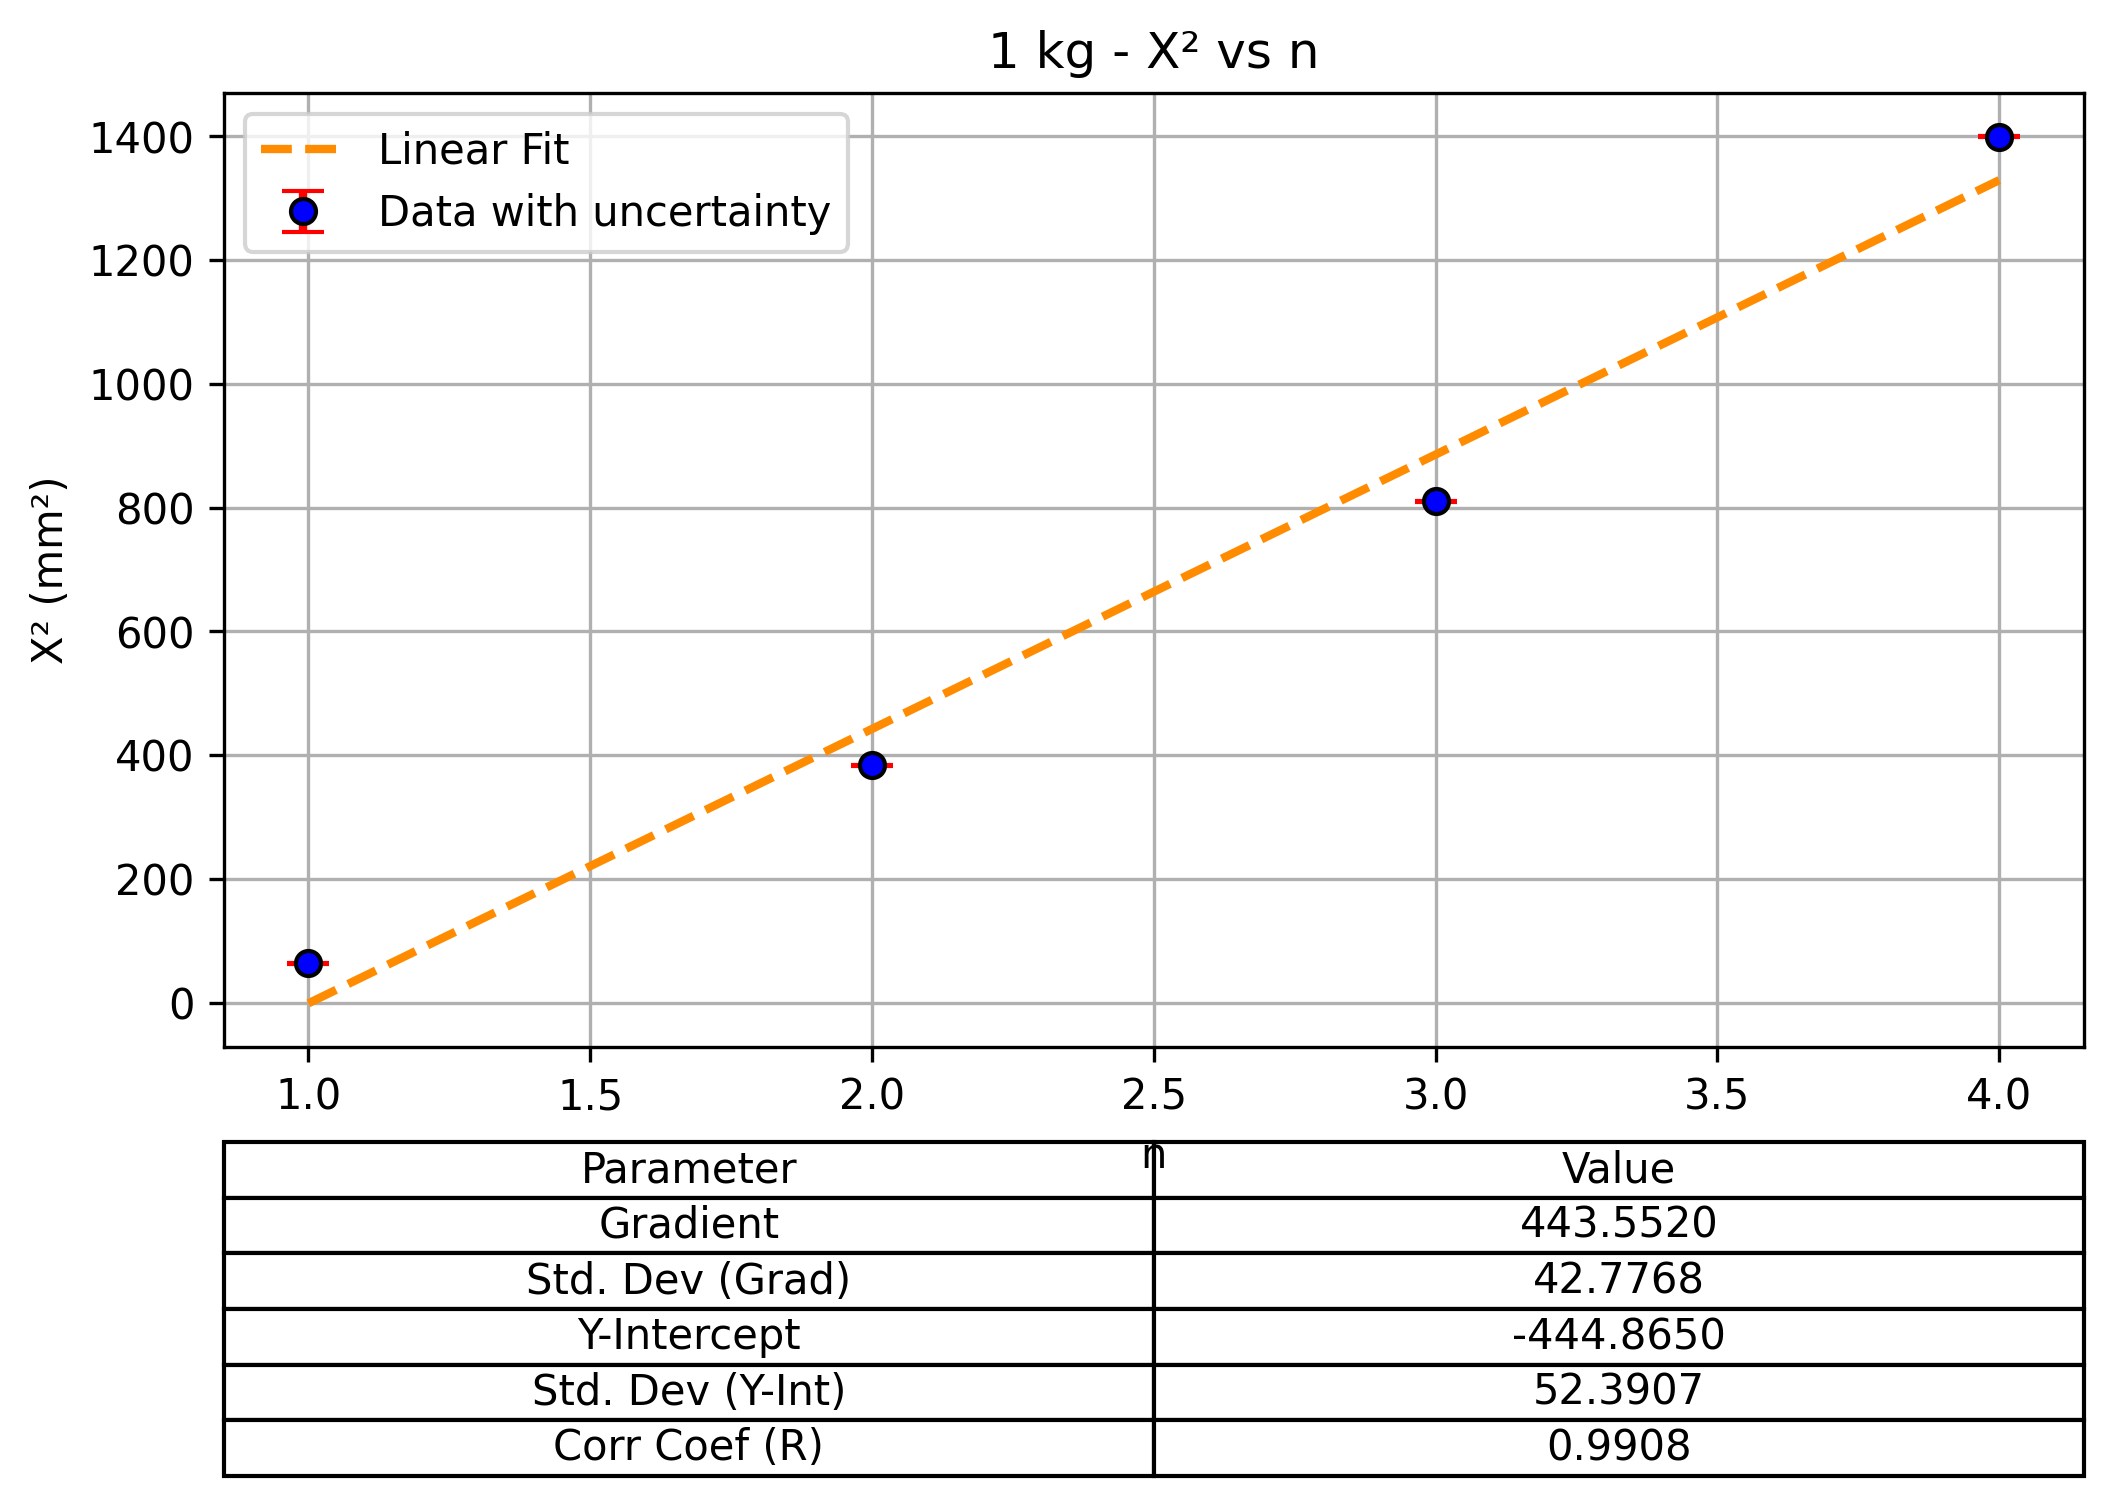
\includegraphics[width=\textwidth]{1kg_X2_vs_n_with_errorbar.png}
    \caption{1 kg -- \(X^2\) vs. \(n\) with linear fit and uncertainties.}
    \label{fig:1kgX2vsn}
  \end{subfigure}
  \hfill
  % First row: right subfigure (1 kg -- Y^2 vs. n)
  \begin{subfigure}[b]{0.45\textwidth}
    \centering
    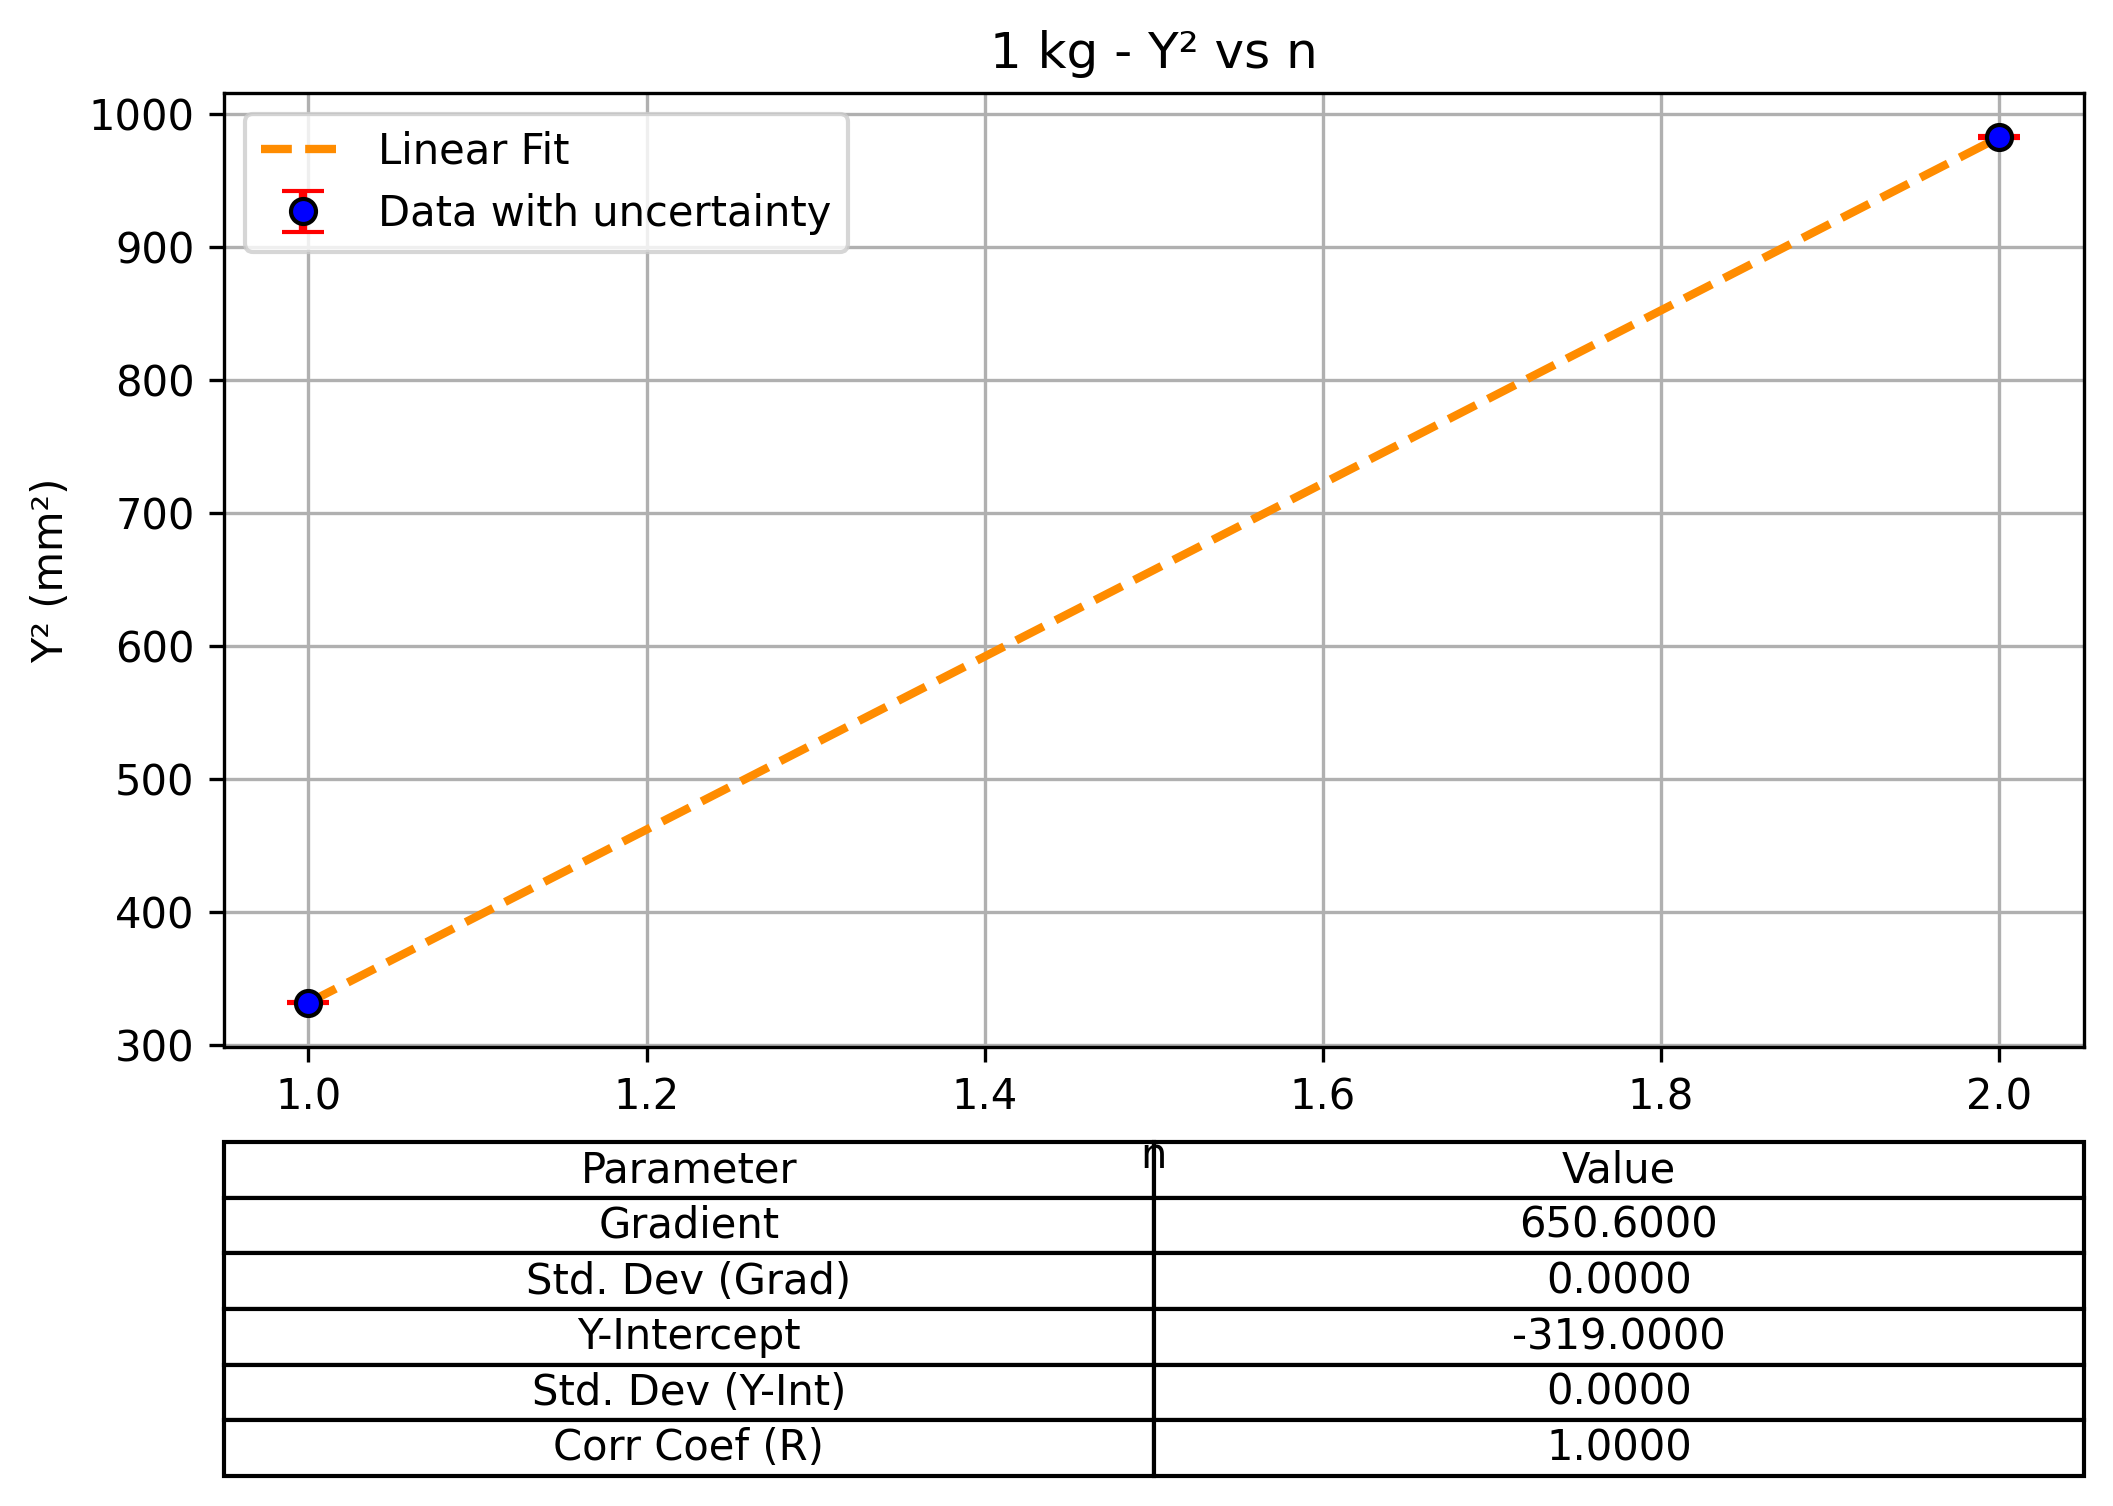
\includegraphics[width=\textwidth]{1kg_Y2_vs_n_with_errorbar.png}
    \caption{1 kg -- \(Y^2\) vs. \(n\) with linear fit and uncertainties.}
    \label{fig:1kgY2vsn}
  \end{subfigure}
  
  \vspace{1em} % Adjust vertical space between rows if needed
  
  % Second row: left subfigure (3 kg -- X^2 vs. n)
  \begin{subfigure}[b]{0.45\textwidth}
    \centering
    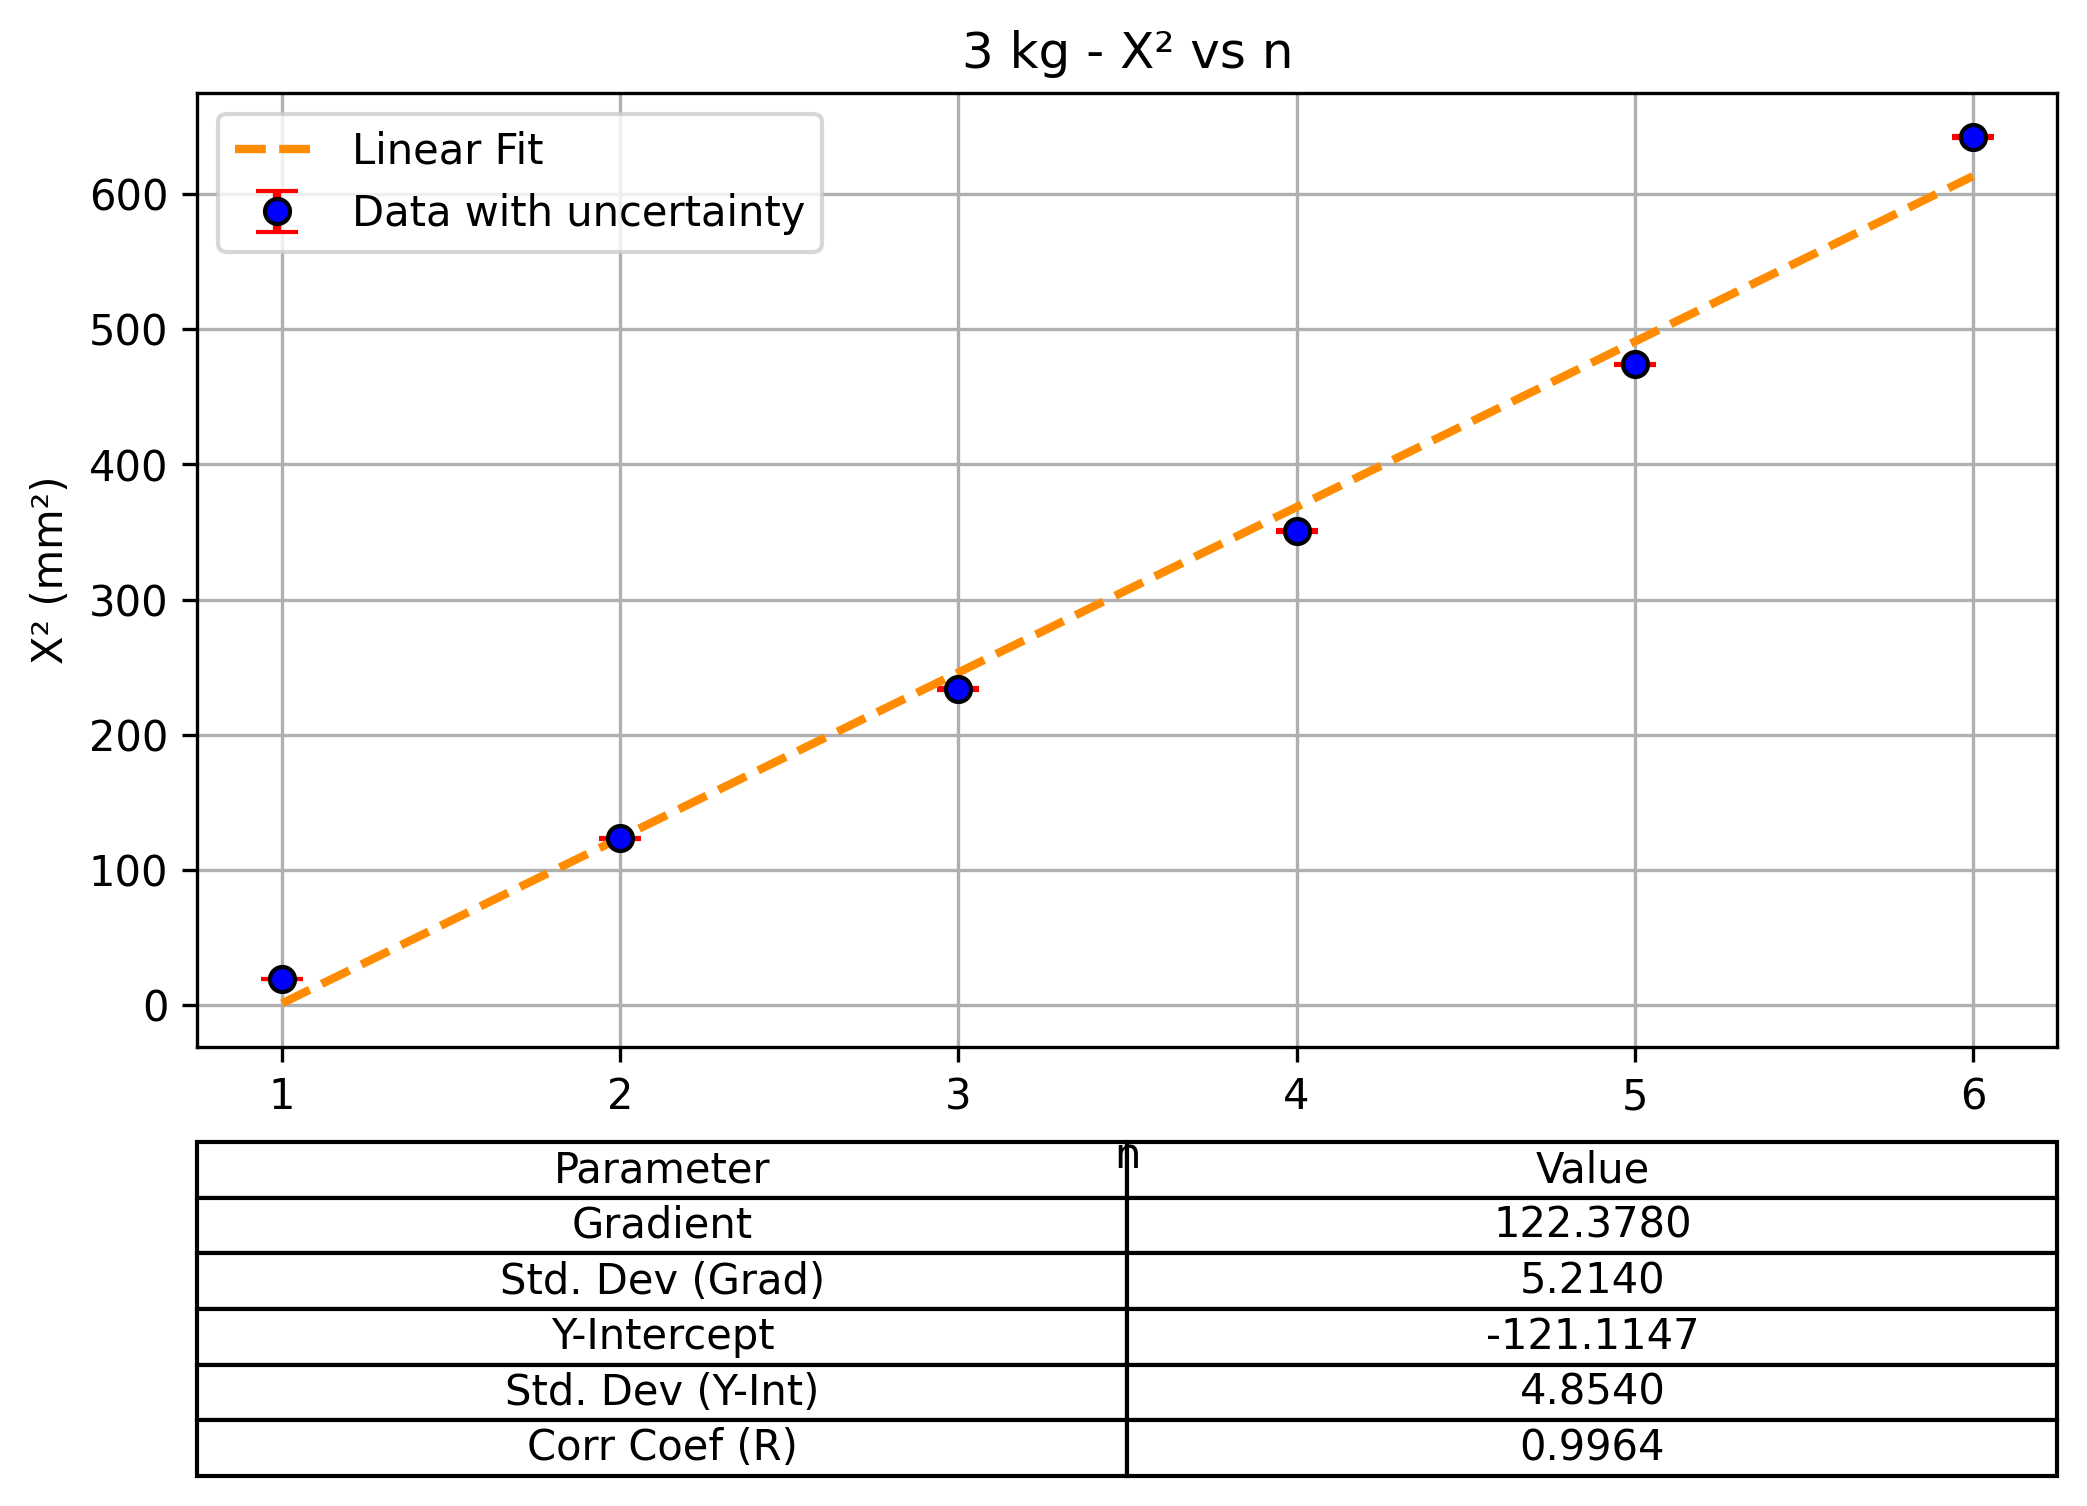
\includegraphics[width=\textwidth]{3kg_X2_vs_n_with_errorbar.png}
    \caption{3 kg -- \(X^2\) vs. \(n\) with linear fit and uncertainties.}
    \label{fig:3kgX2vsn}
  \end{subfigure}
  \hfill
  % Second row: right subfigure (3 kg -- Y^2 vs. n)
  \begin{subfigure}[b]{0.45\textwidth}
    \centering
    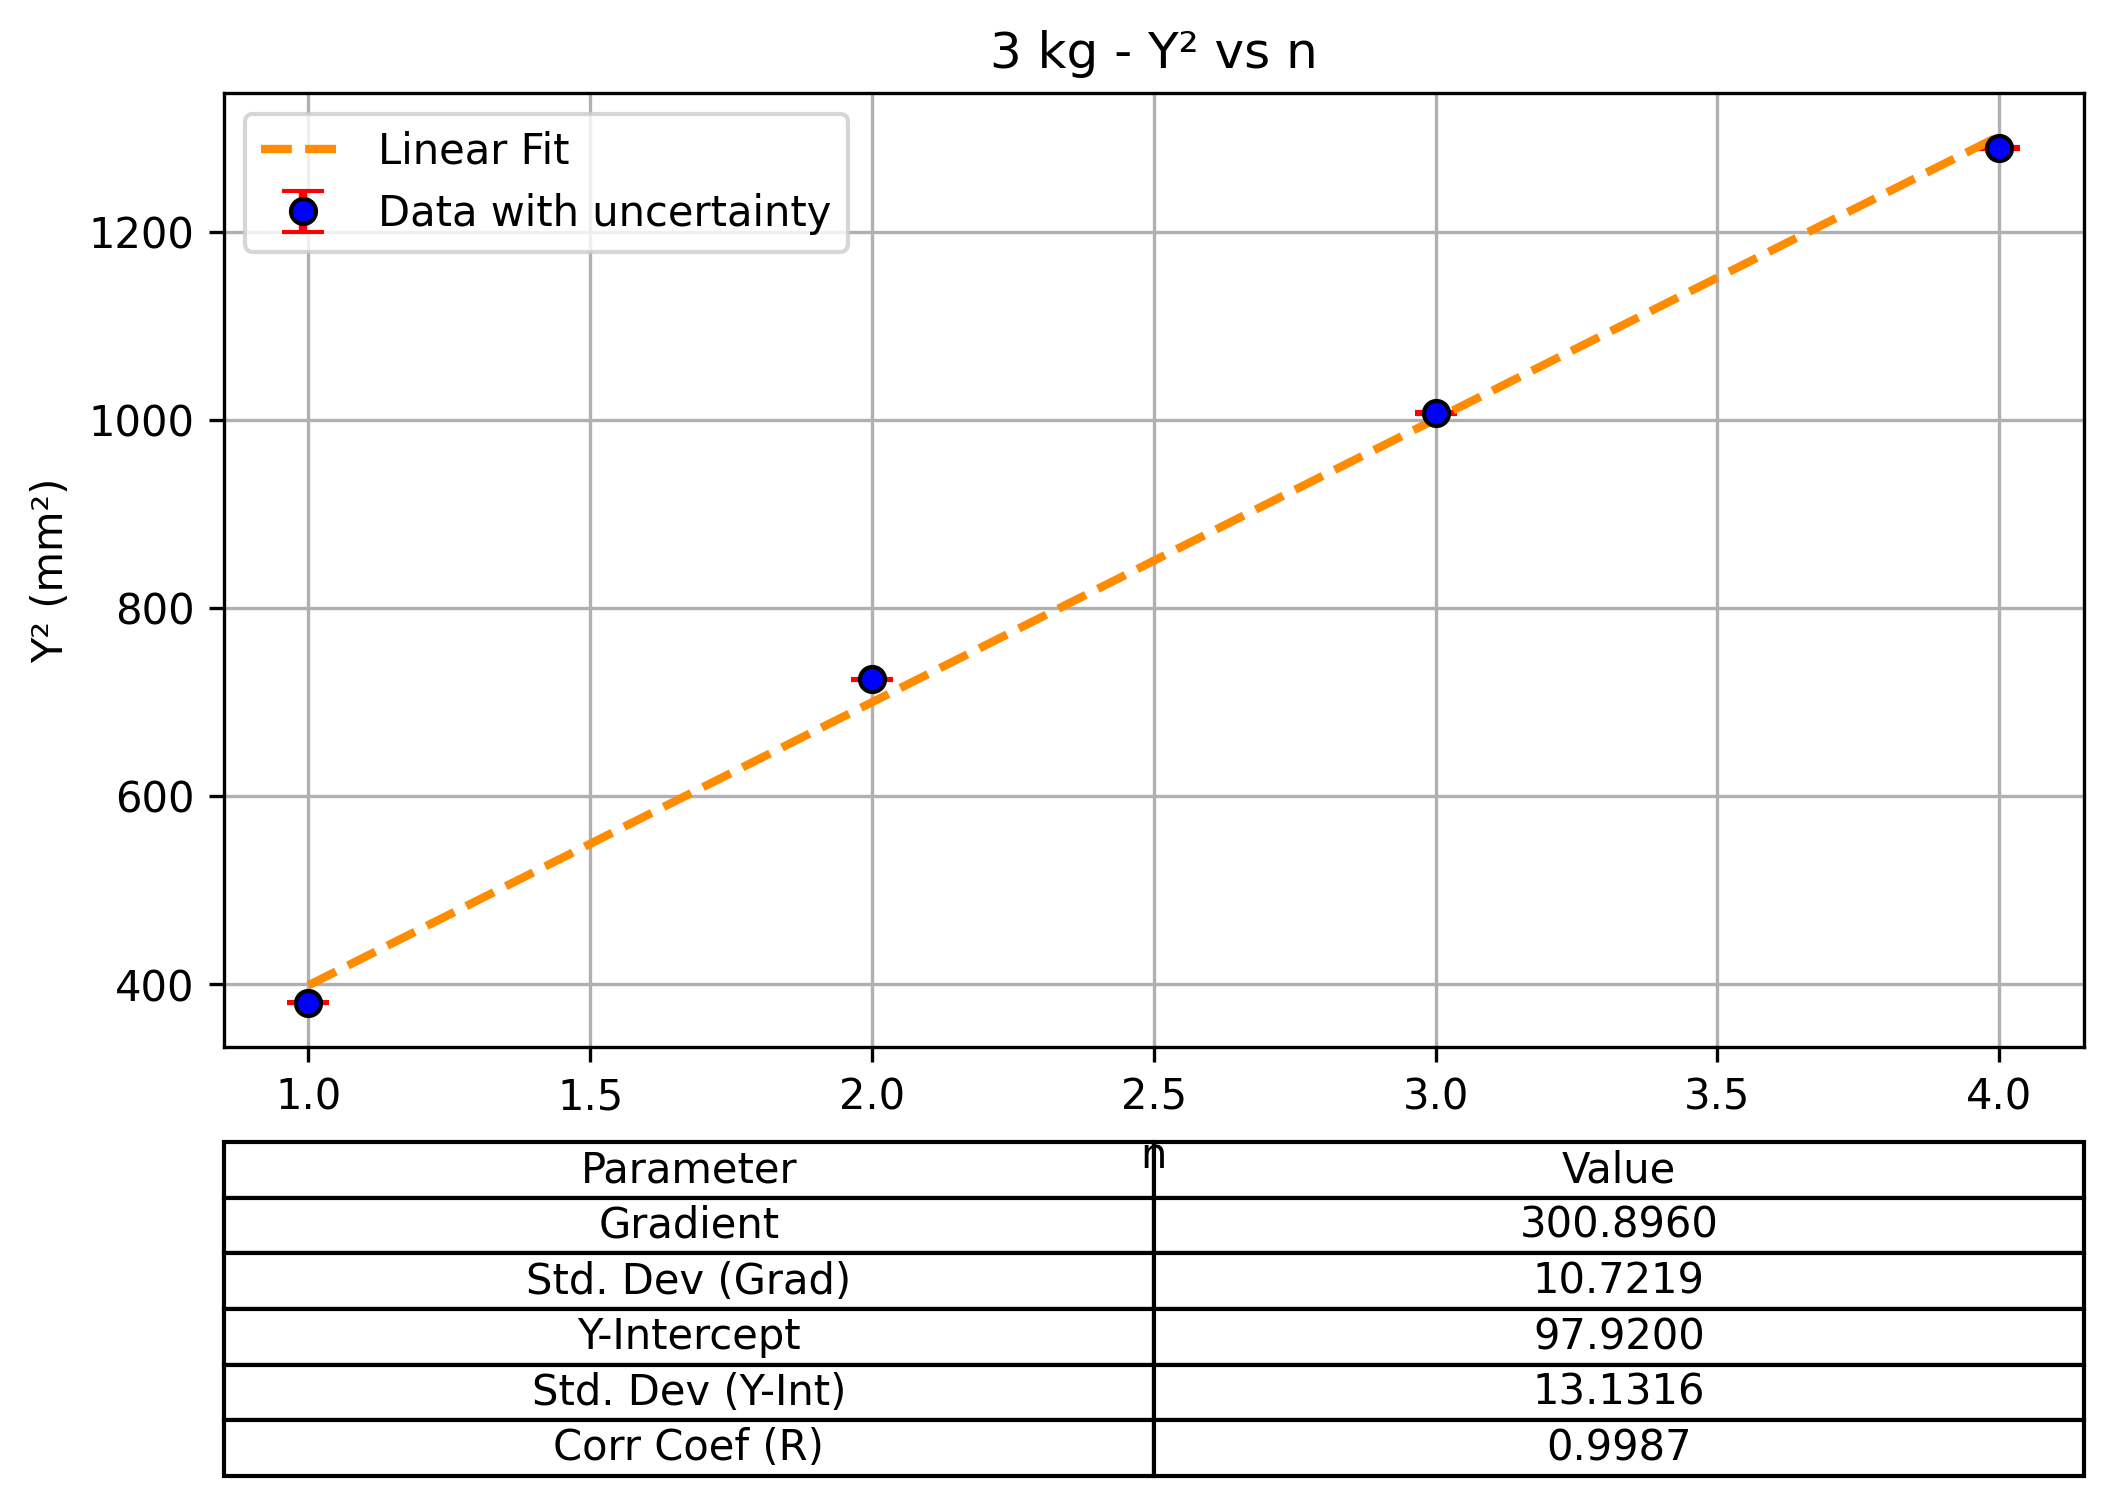
\includegraphics[width=\textwidth]{3kg_Y2_vs_n_with_errorbar.png}
    \caption{3 kg -- \(Y^2\) vs. \(n\) with linear fit and uncertainties.}
    \label{fig:3kgY2vsn}
  \end{subfigure}
  
  \caption{Linear regressions for \(X^2\) and \(Y^2\) versus \(n\) for 1 kg and 3 kg loads. The regression parameters (displayed below each plot) include uncertainties.}
  \label{fig:fits}
\end{figure}

\begin{figure}[H]
  \centering
  % Row 1: 4 kg plots
  \begin{subfigure}[b]{0.45\textwidth}
    \centering
    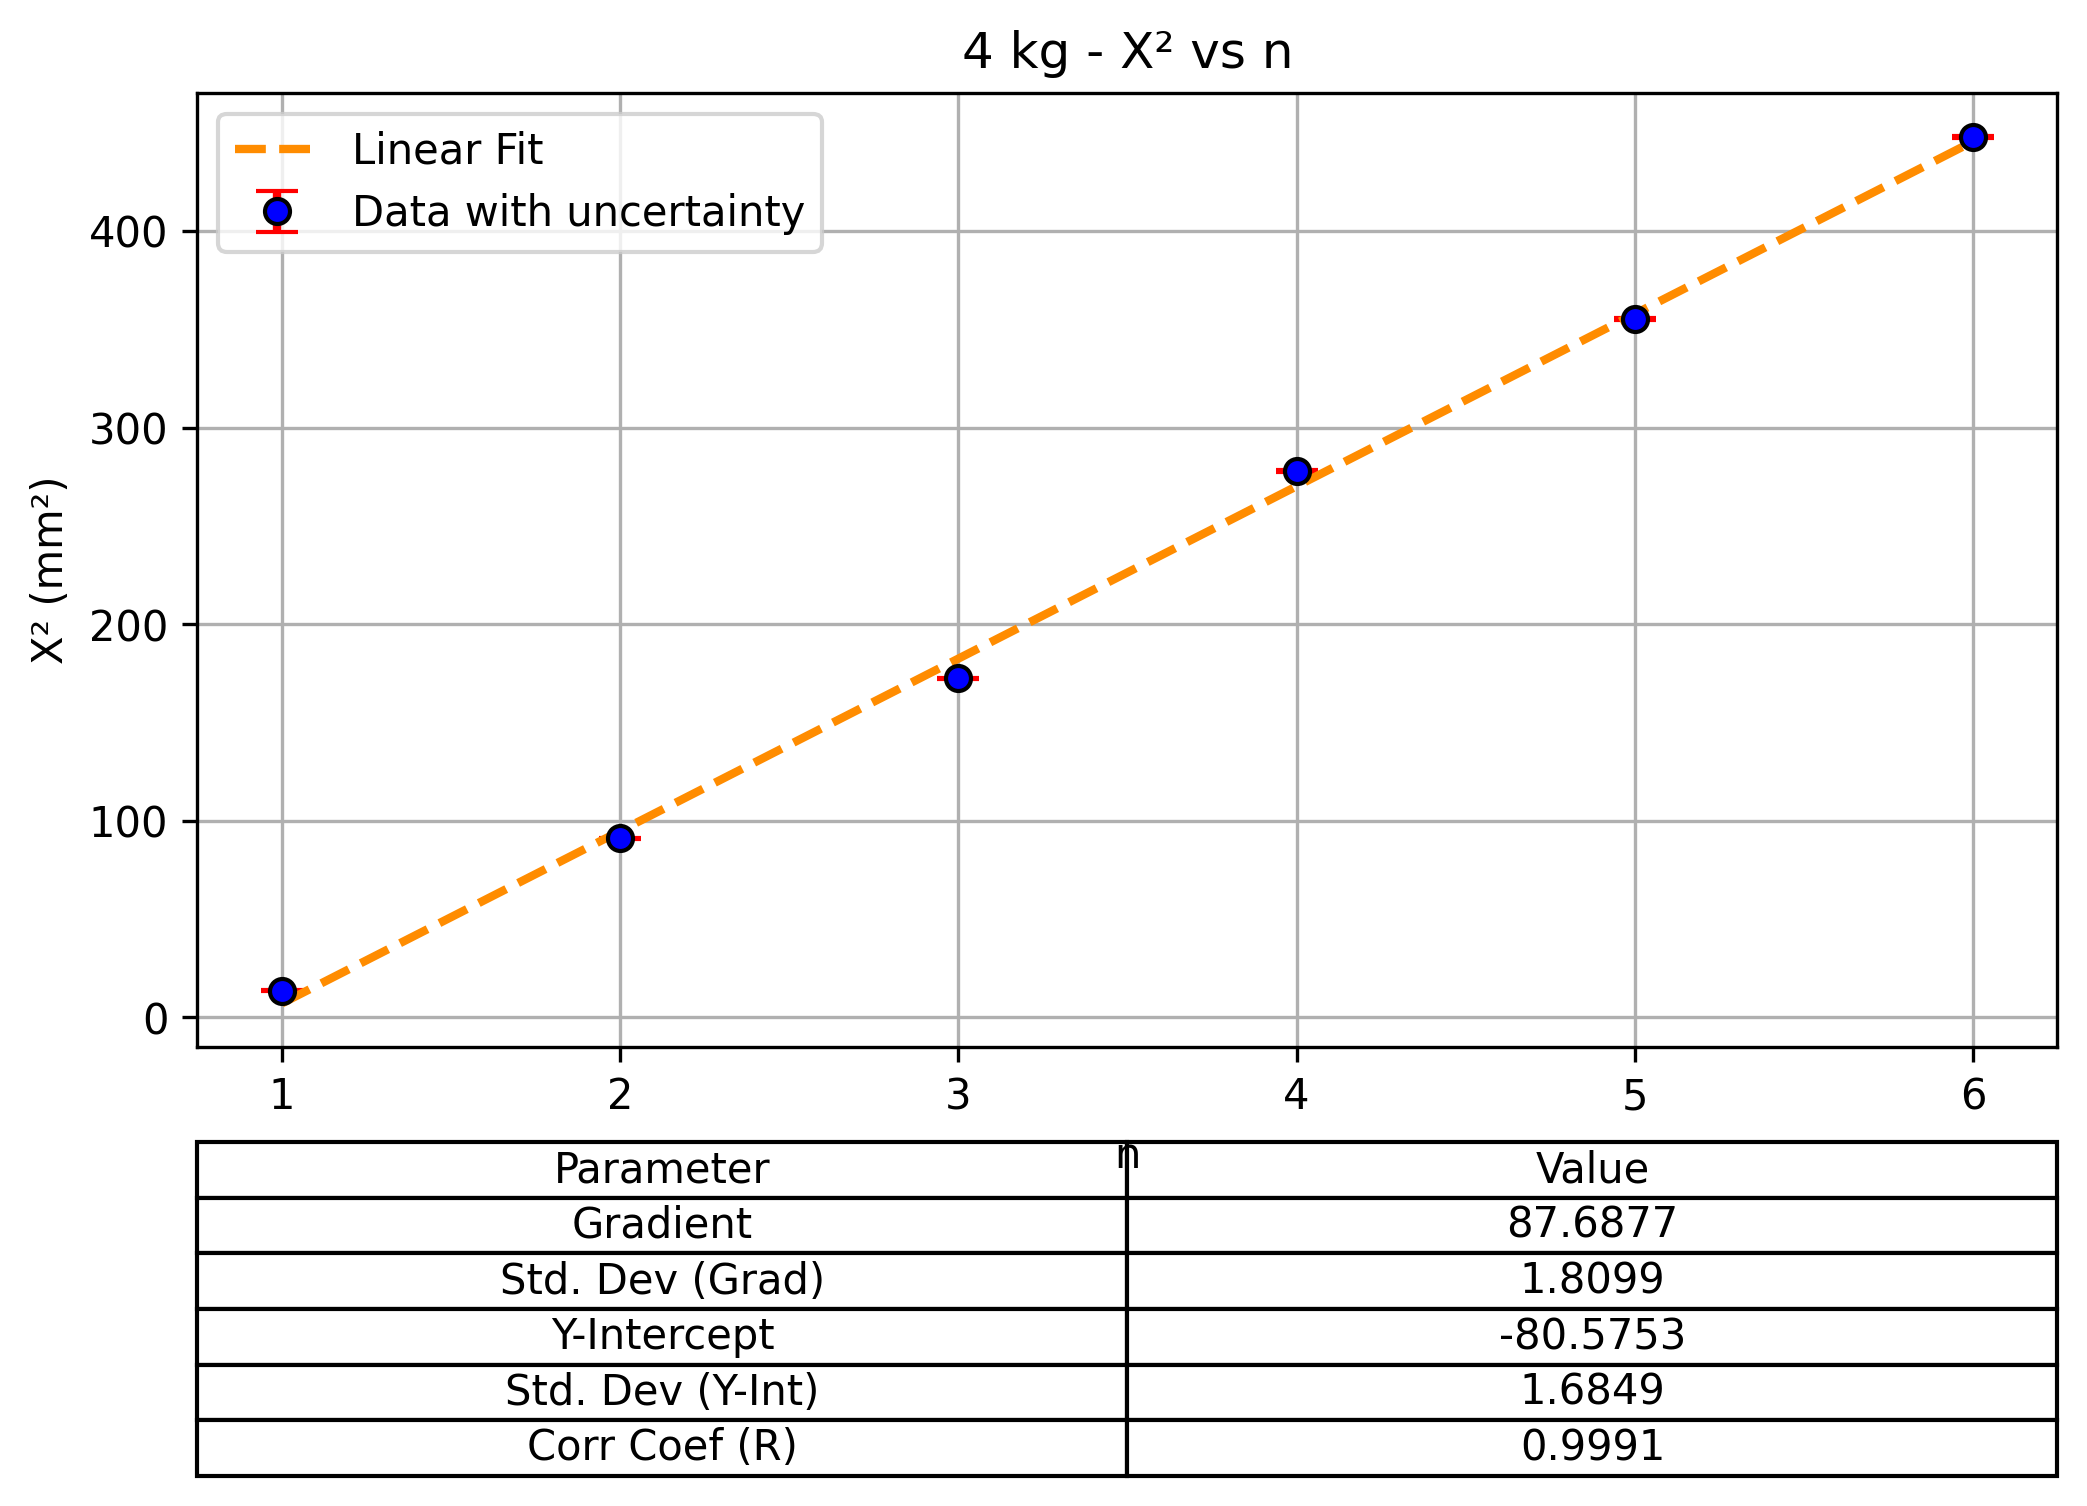
\includegraphics[width=\textwidth]{4kg_X2_vs_n_with_errorbar.png}
    \caption{4 kg -- \(X^2\) vs. \(n\) with linear fit and uncertainties.}
    \label{fig:4kgX2vsn}
  \end{subfigure}
  \hfill
  \begin{subfigure}[b]{0.45\textwidth}
    \centering
    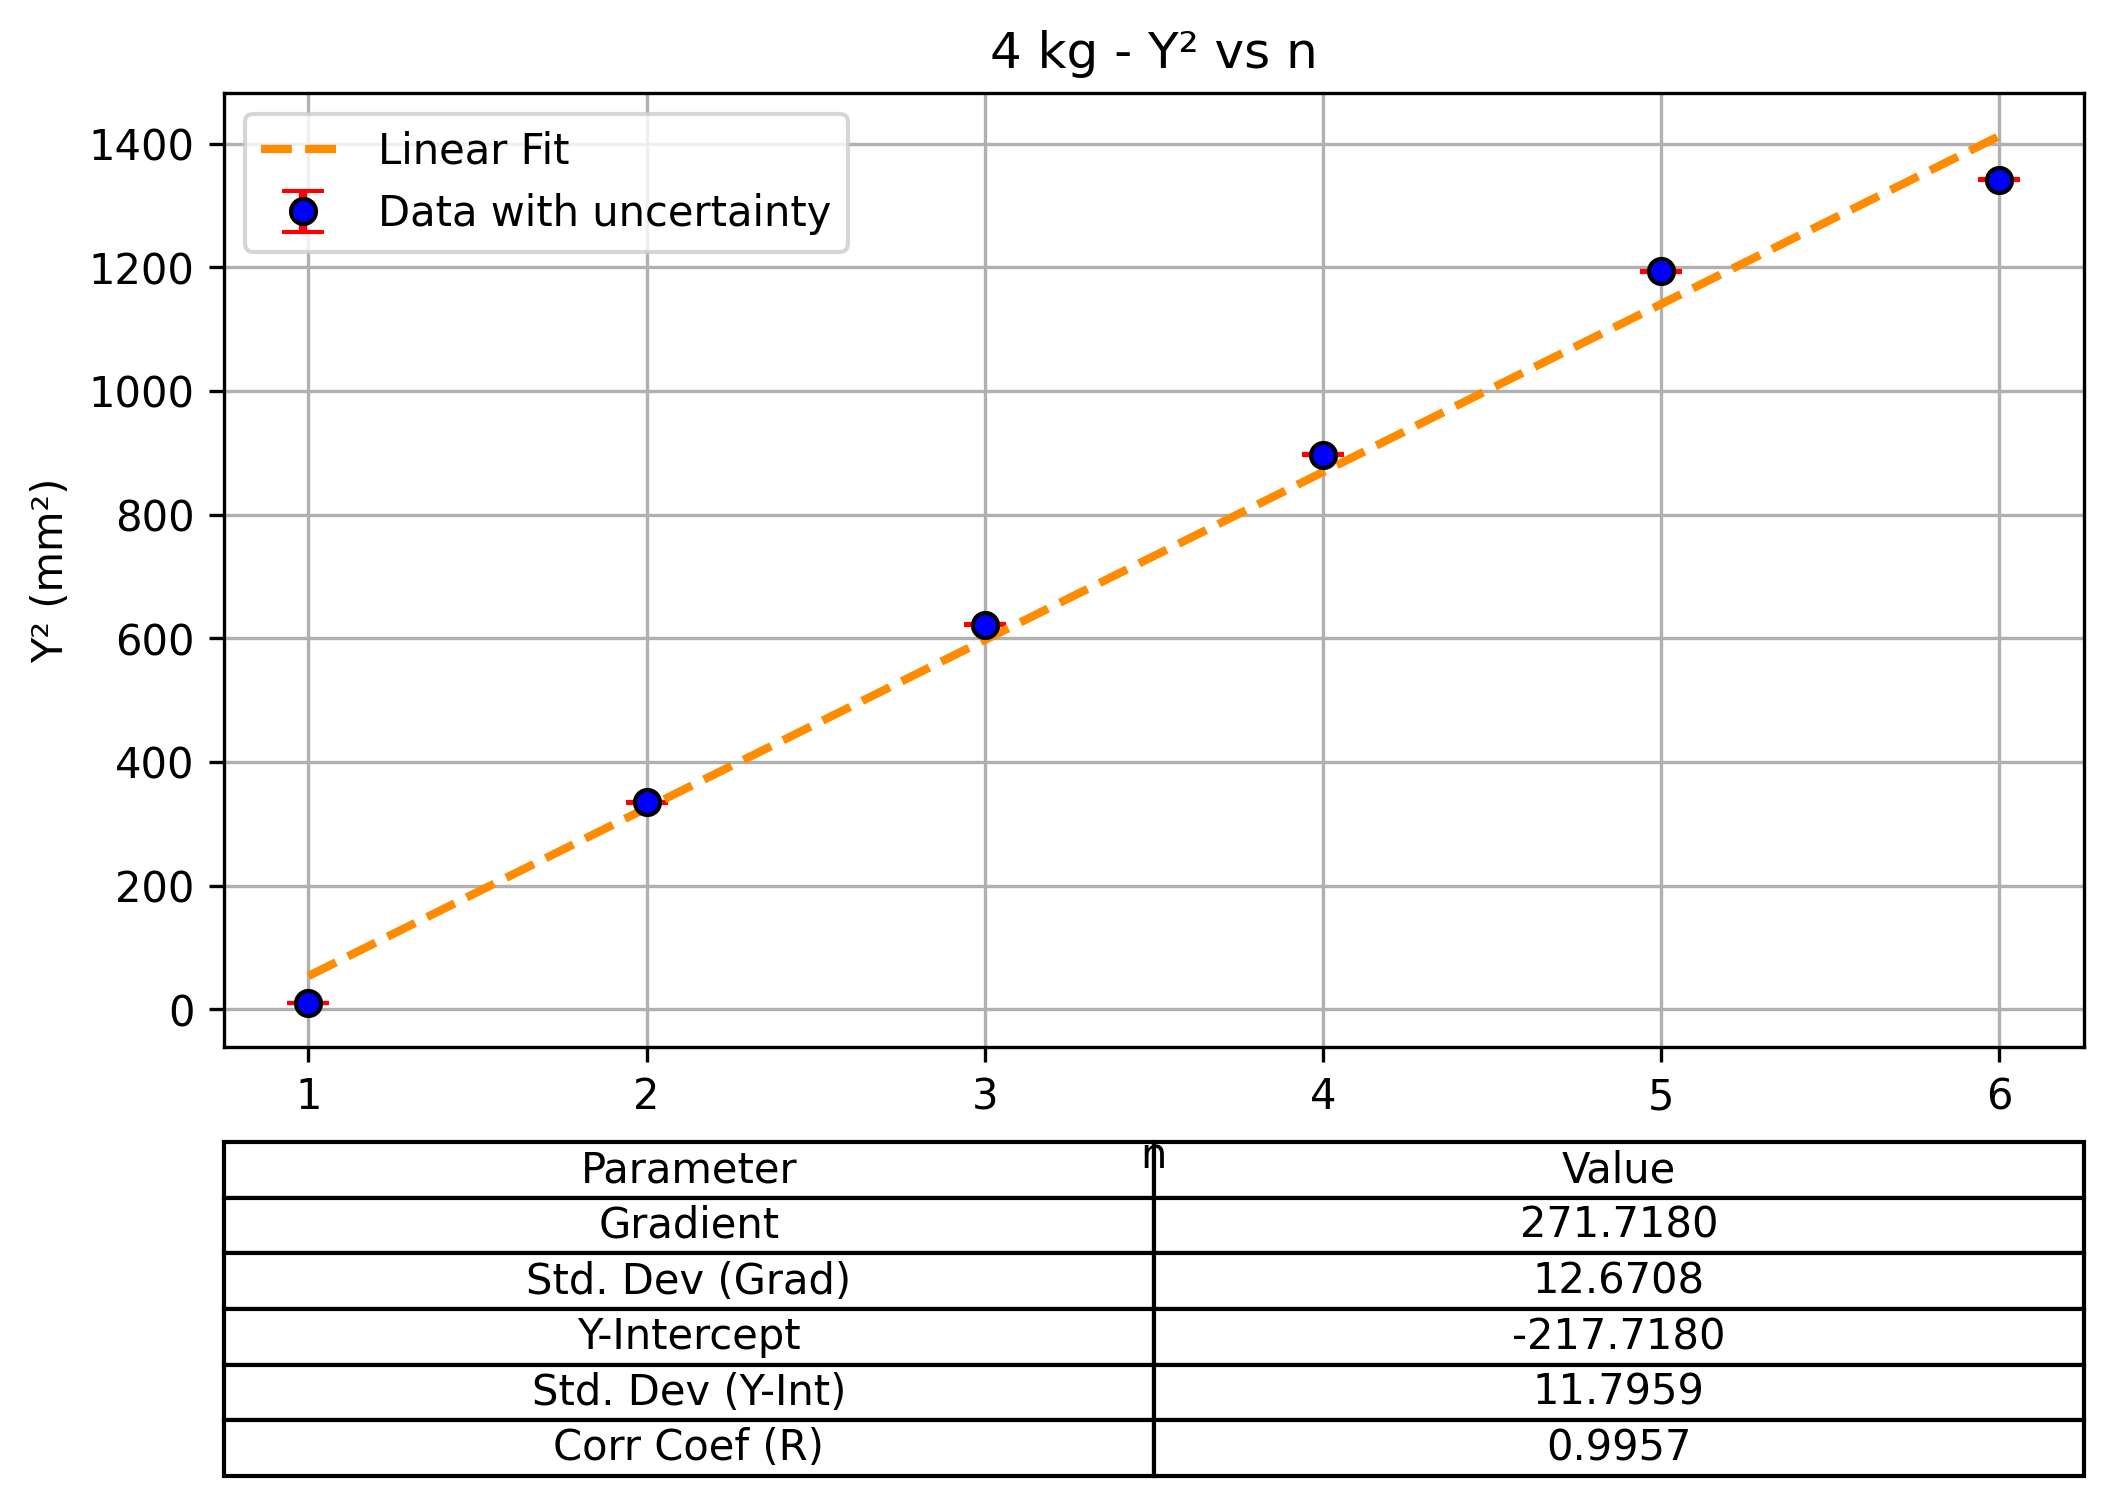
\includegraphics[width=\textwidth]{4kg_Y2_vs_n_with_errorbar.png}
    \caption{4 kg -- \(Y^2\) vs. \(n\) with linear fit and uncertainties.}
    \label{fig:4kgY2vsn}
  \end{subfigure}
  
  \vspace{1em} % Vertical space between rows
  
  % Row 2: 5 kg plots
  \begin{subfigure}[b]{0.45\textwidth}
    \centering
    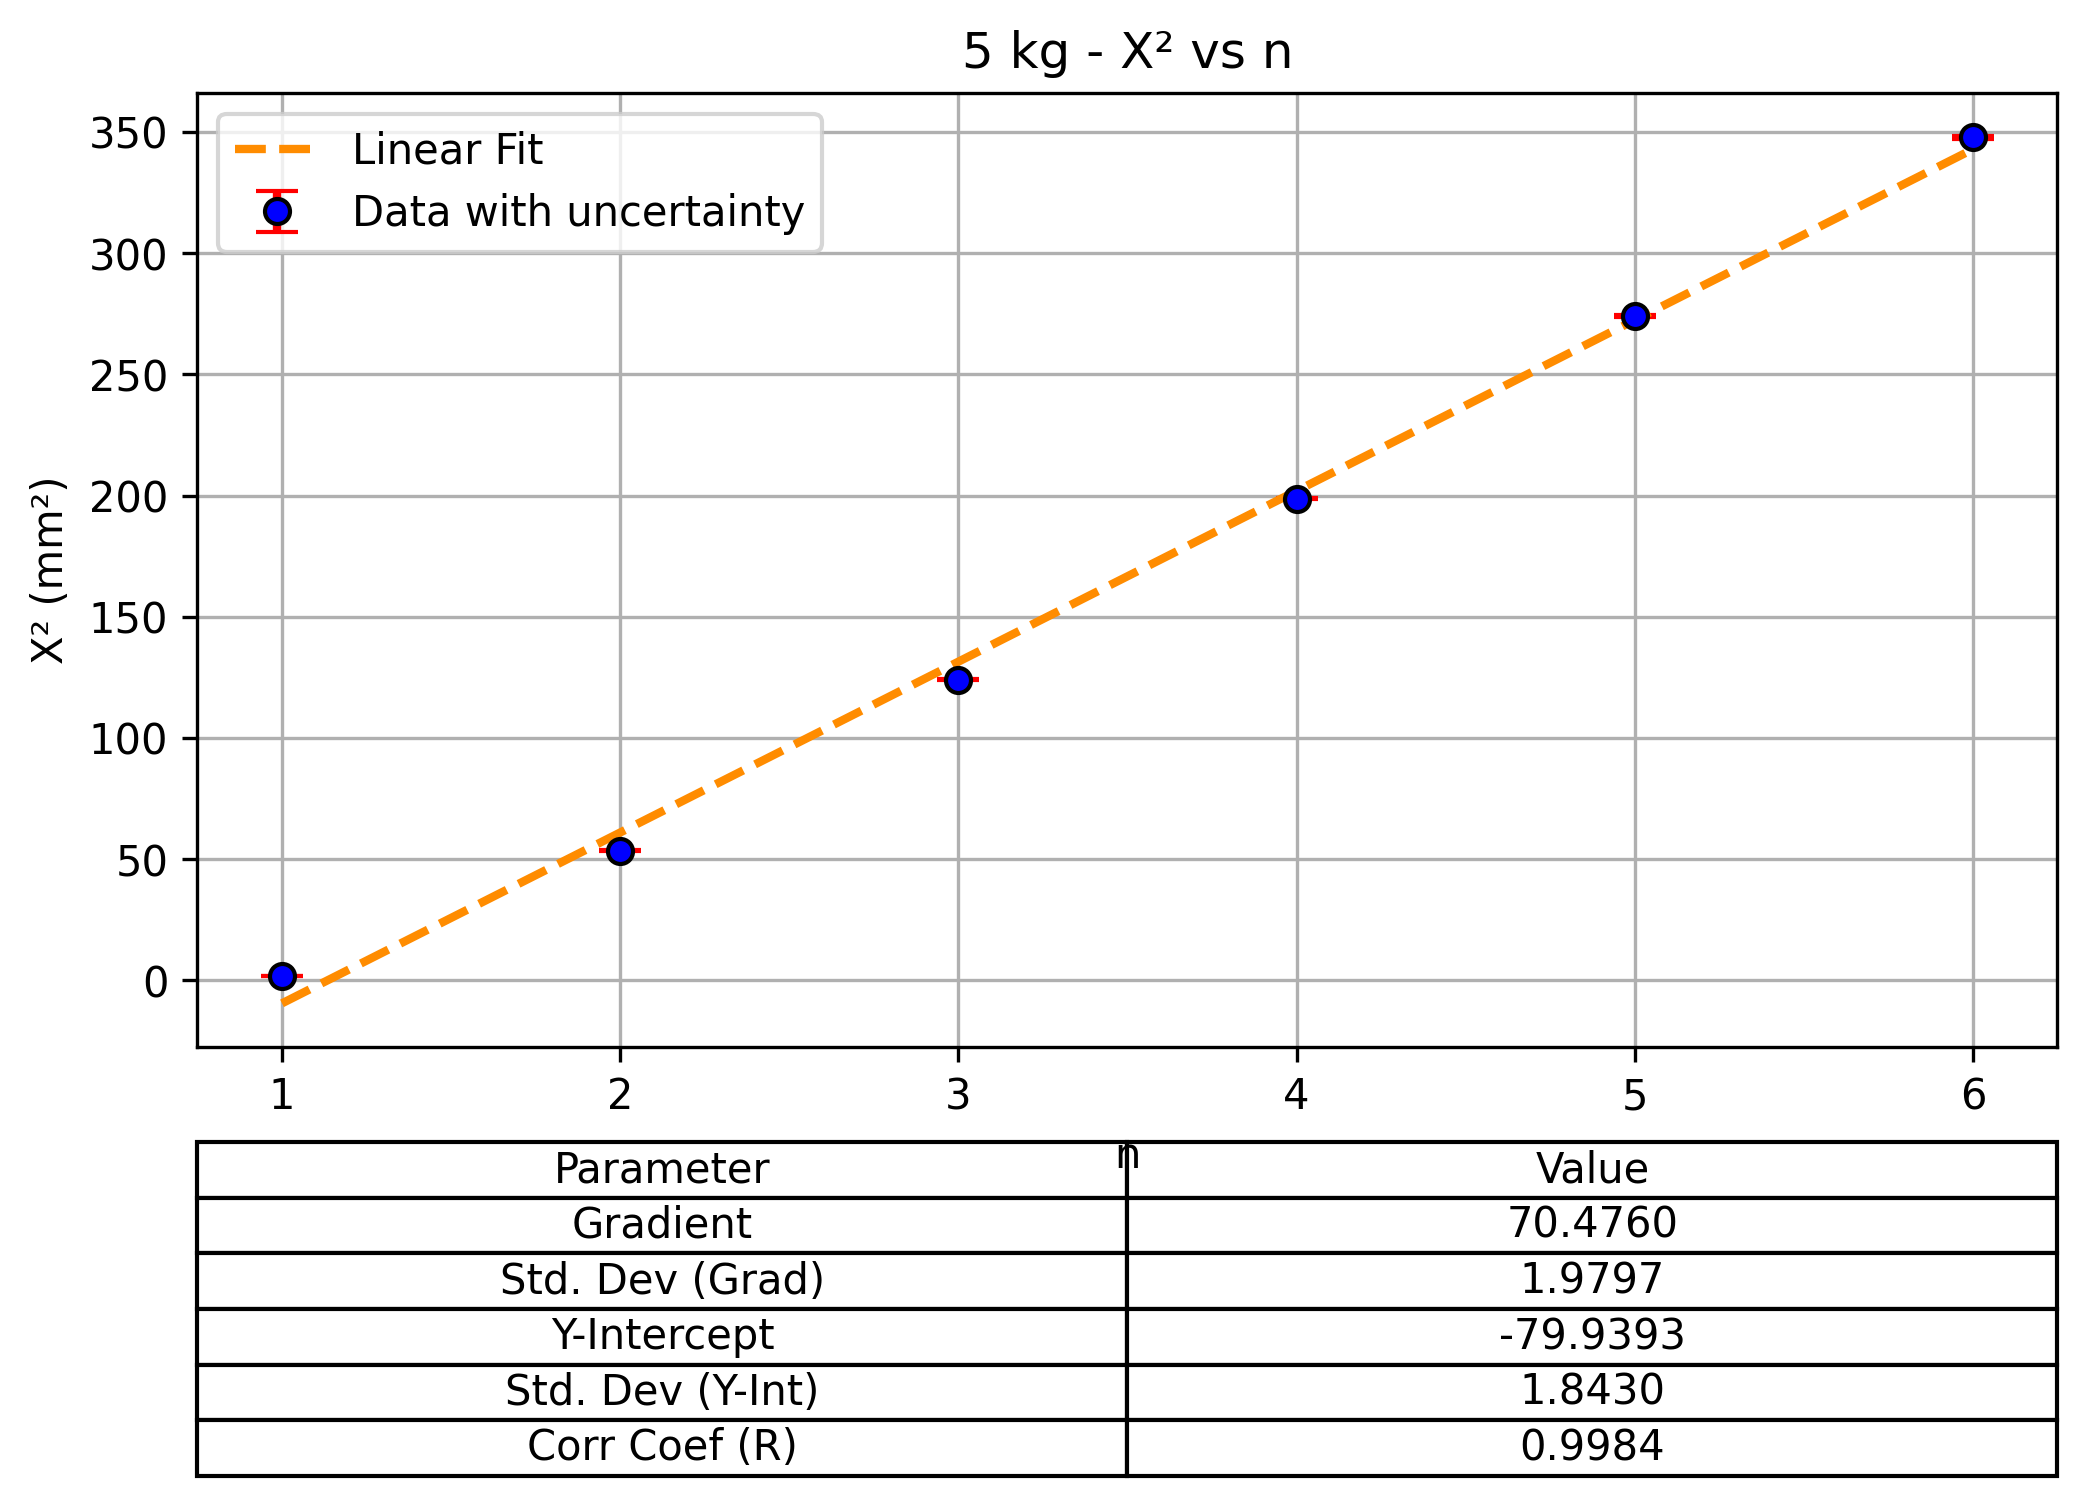
\includegraphics[width=\textwidth]{5kg_X2_vs_n_with_errorbar.png}
    \caption{5 kg -- \(X^2\) vs. \(n\) with linear fit and uncertainties.}
    \label{fig:5kgX2vsn}
  \end{subfigure}
  \hfill
  \begin{subfigure}[b]{0.45\textwidth}
    \centering
    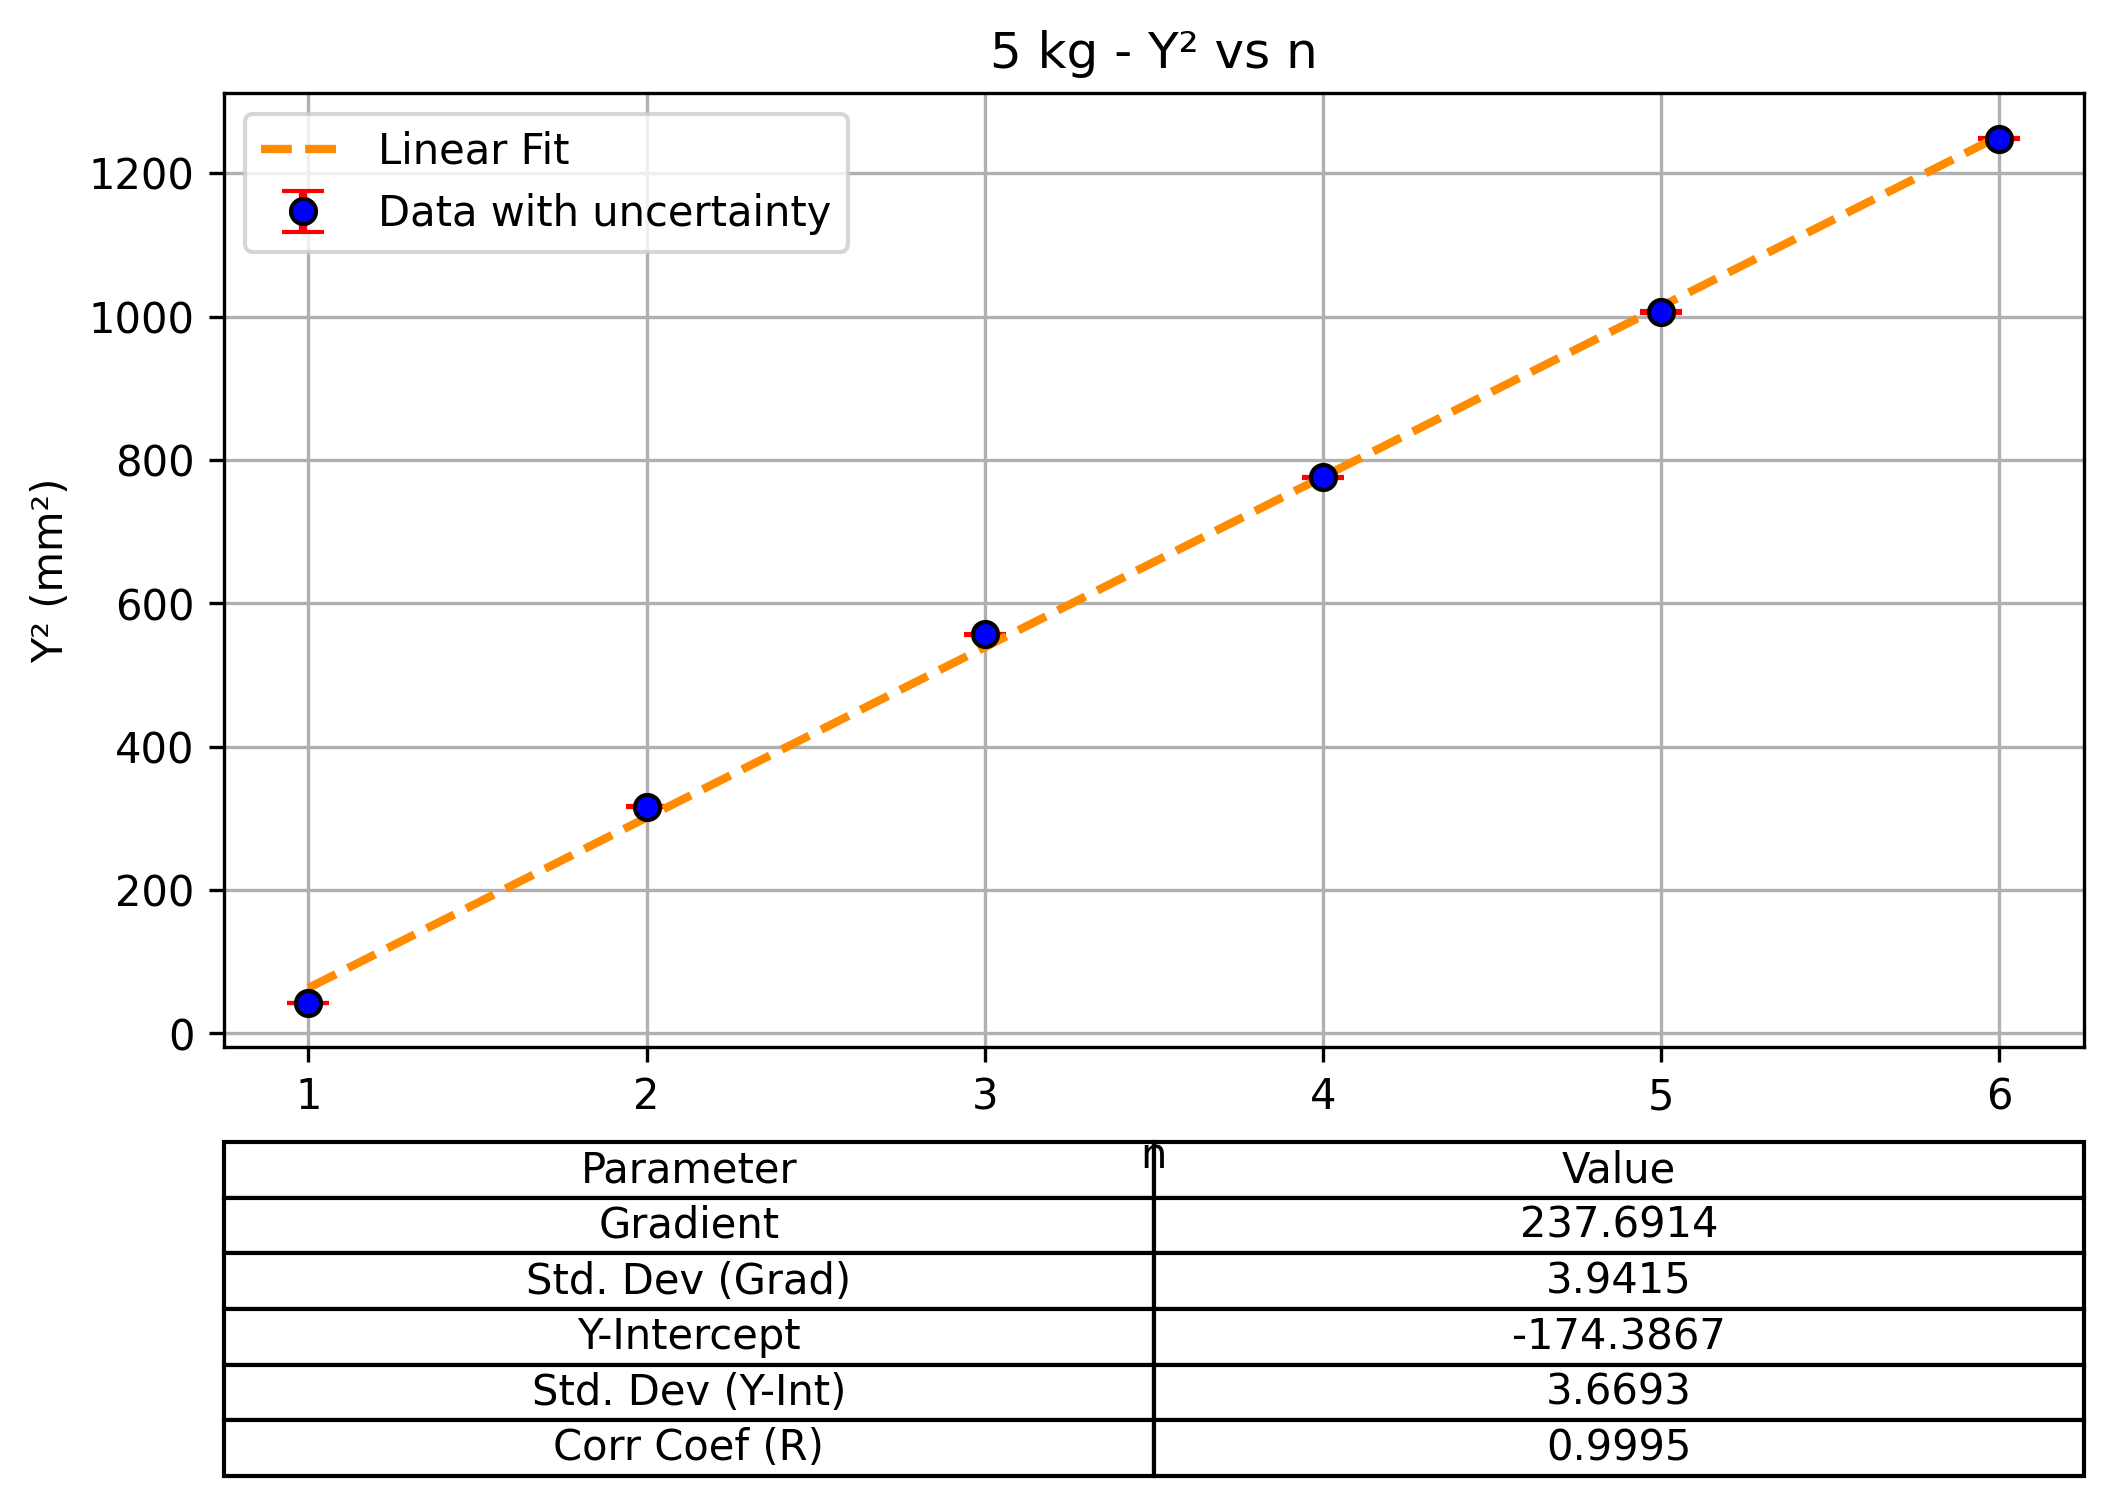
\includegraphics[width=\textwidth]{5kg_Y2_vs_n_with_errorbar.png}
    \caption{5 kg -- \(Y^2\) vs. \(n\) with linear fit and uncertainties.}
    \label{fig:5kgY2vsn}
  \end{subfigure}
  
  \vspace{1em} % Vertical space between rows
  
  % Row 3: 6 kg plots
  \begin{subfigure}[b]{0.45\textwidth}
    \centering
    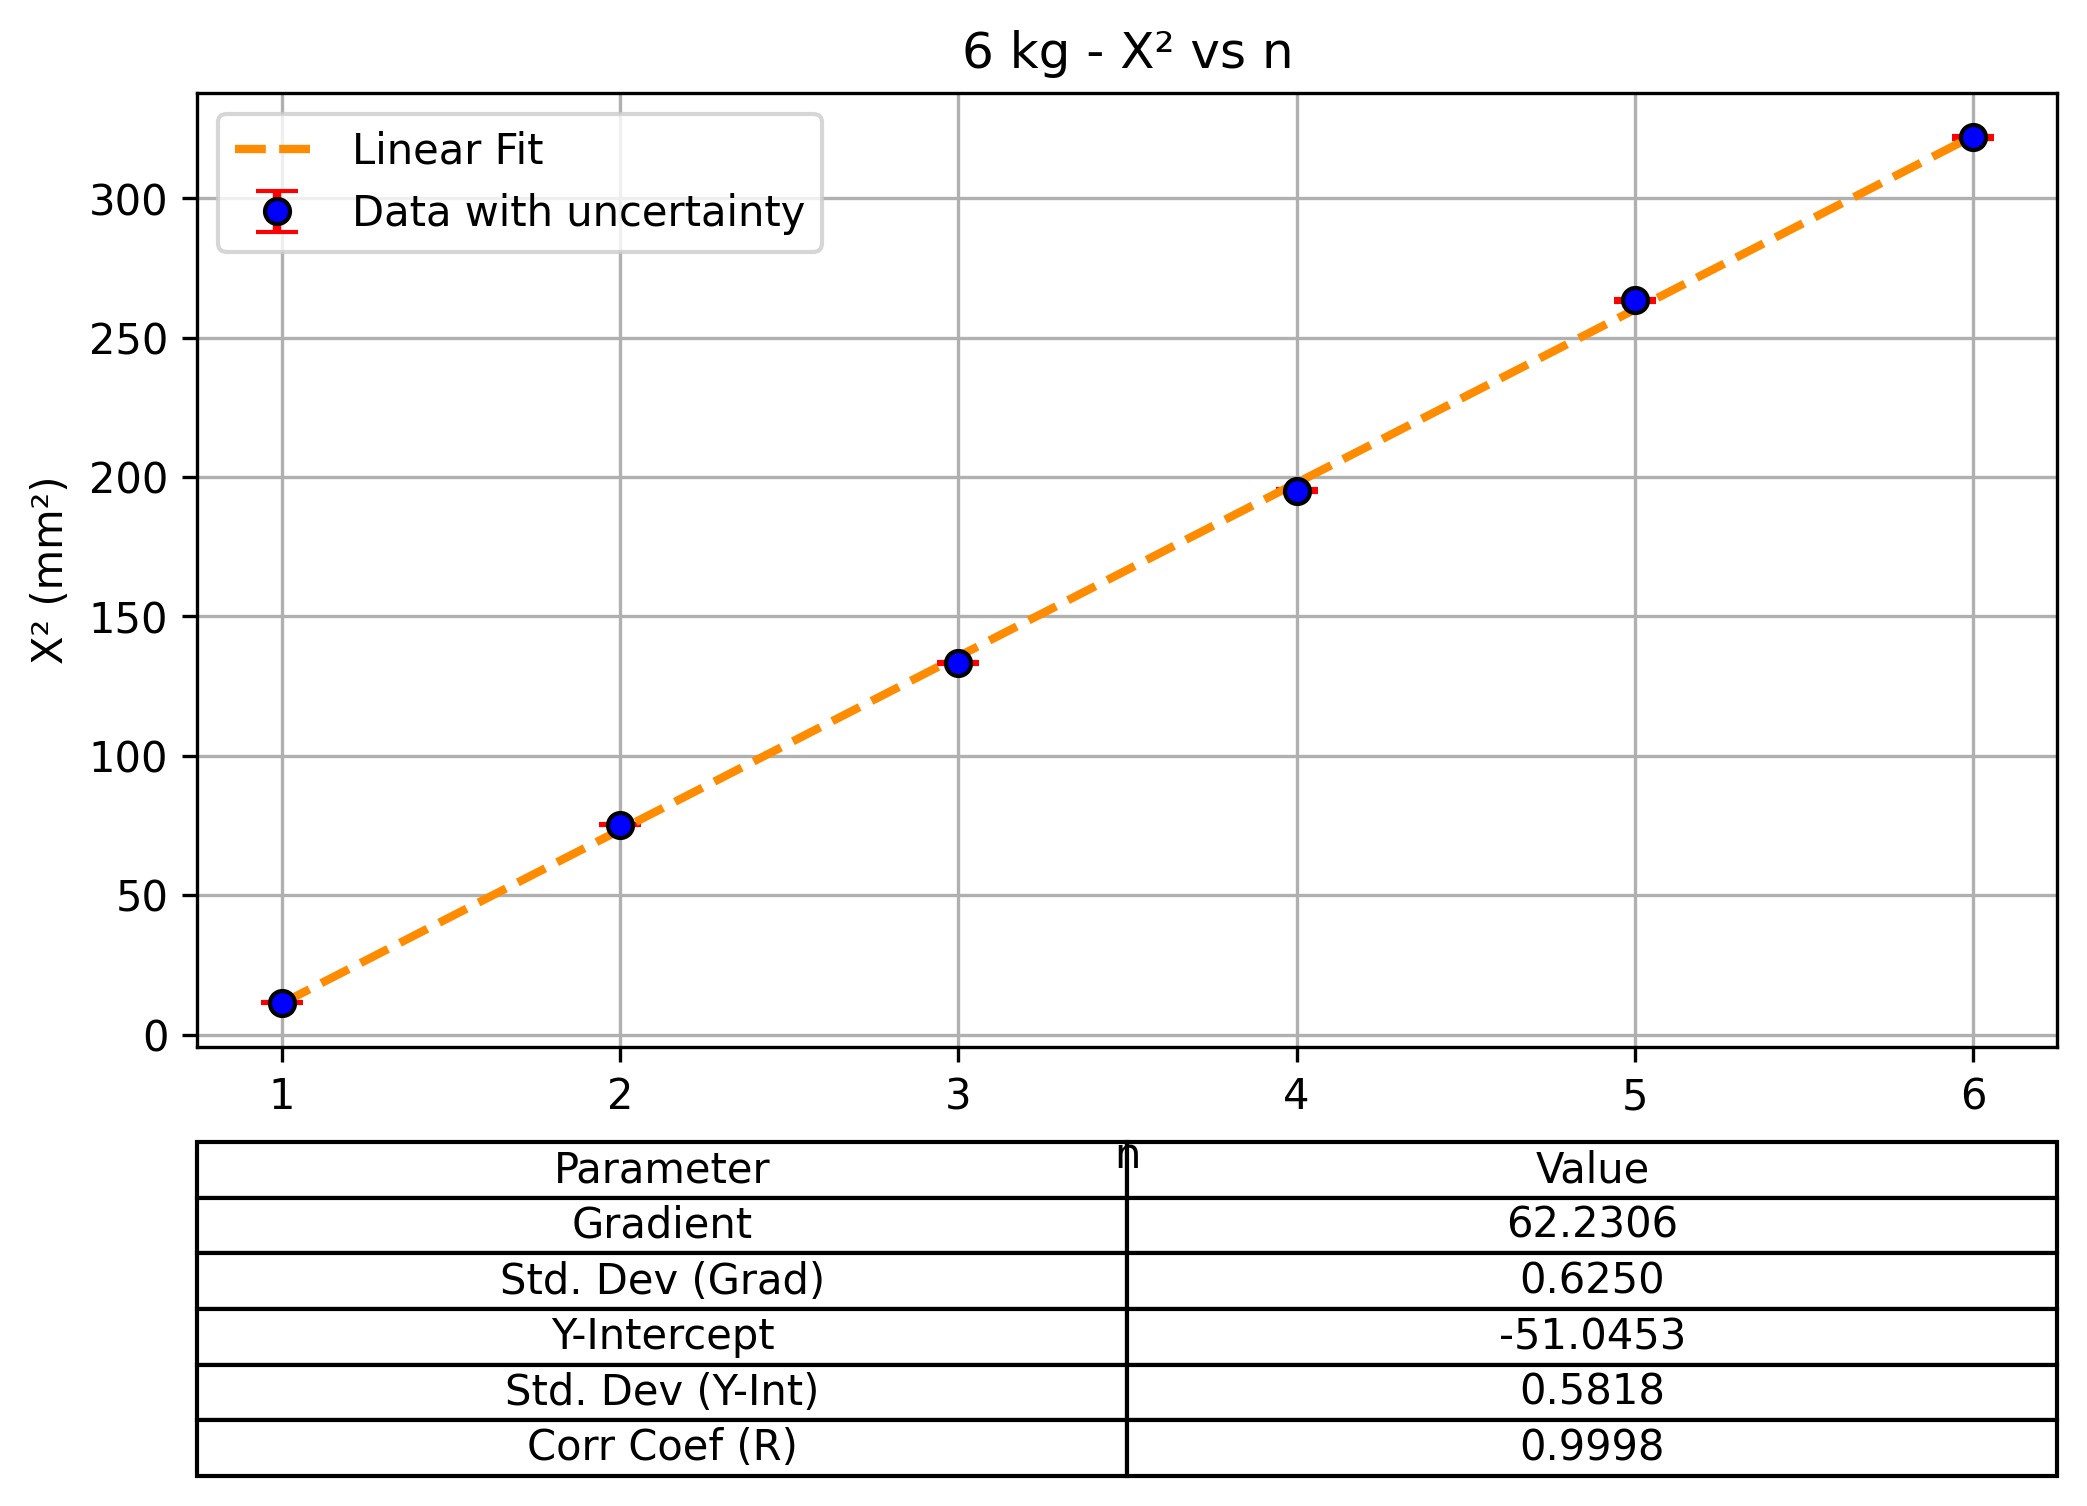
\includegraphics[width=\textwidth]{6kg_X2_vs_n_with_errorbar.png}
    \caption{6 kg -- \(X^2\) vs. \(n\) with linear fit and uncertainties.}
    \label{fig:6kgX2vsn}
  \end{subfigure}
  \hfill
  \begin{subfigure}[b]{0.45\textwidth}
    \centering
    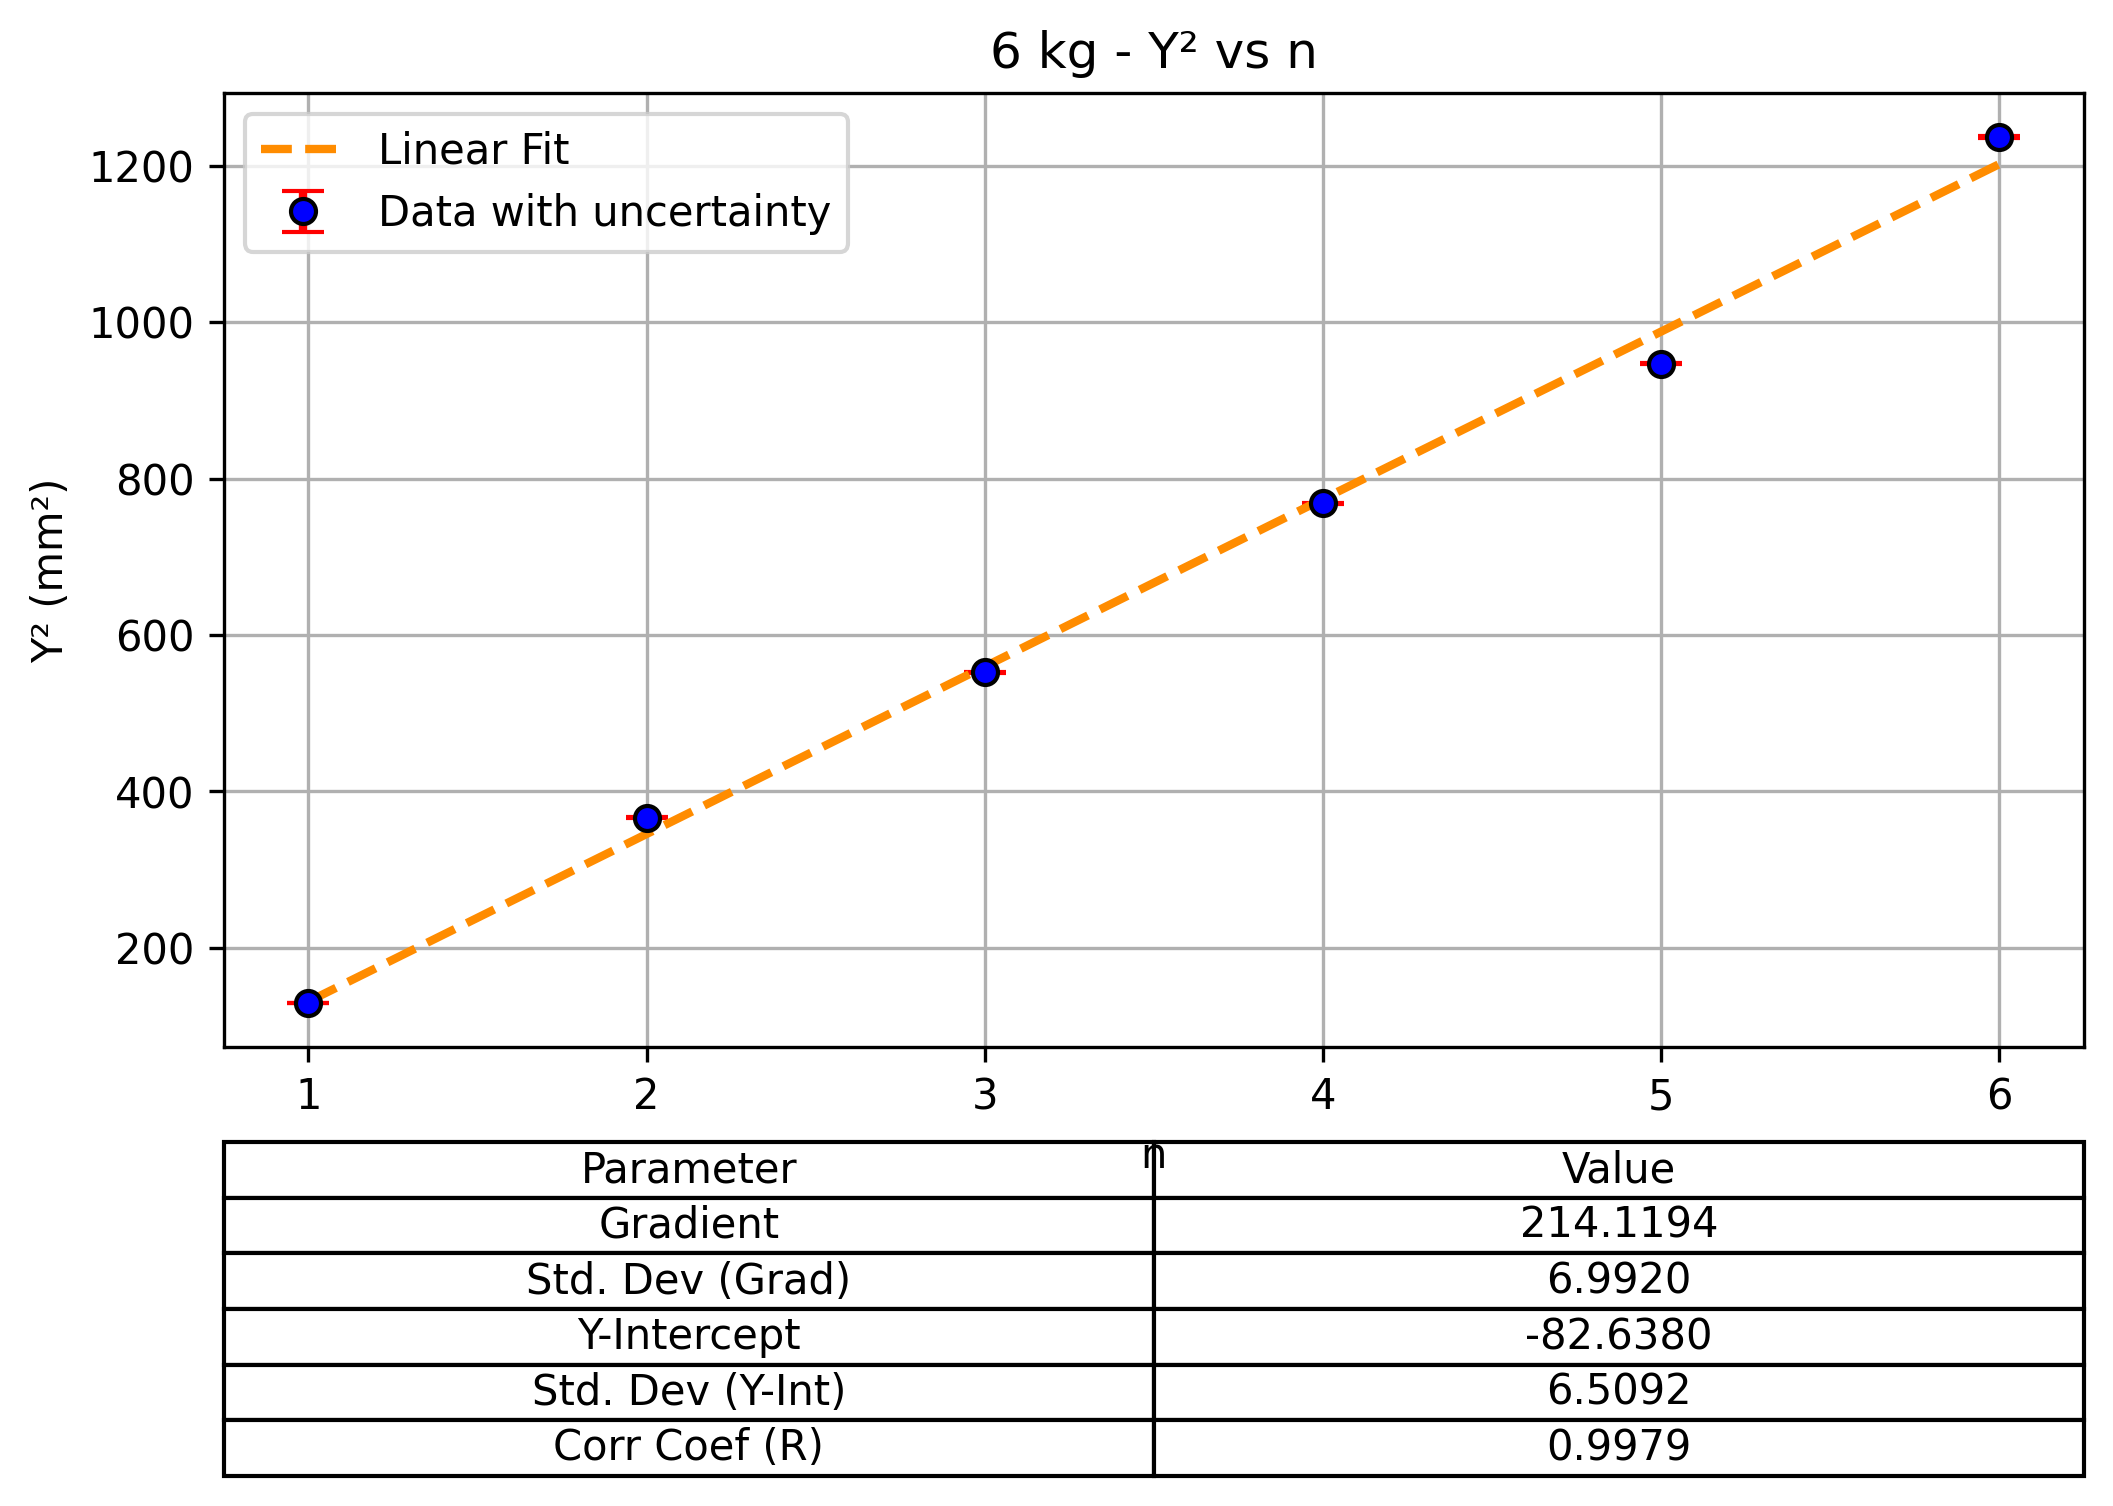
\includegraphics[width=\textwidth]{6kg_Y2_vs_n_with_errorbar.png}
    \caption{6 kg -- \(Y^2\) vs. \(n\) with linear fit and uncertainties.}
    \label{fig:6kgY2vsn}
  \end{subfigure}
  
  \caption{Linear regression plots for \(X^2\) and \(Y^2\) versus \(n\) for 4\,kg, 5\,kg, and 6\,kg loads. Each subfigure shows the data with a linear fit, including the regression parameters and their uncertainties.}
  \label{fig:all_fits}
\end{figure}

The analysis began by recording the interference fringe positions in both the horizontal and vertical orientations for each applied load. For each set of measurements, the fringe displacements were used to compute the squared fringe separations, \(X_n^2\) (horizontal) and \(Y_n^2\) (vertical), which were then plotted against the fringe order \(n\). Linear regression of these plots produced slopes that, according to the theoretical relationship 
\begin{equation}
X_n^2 = 4\,\lambda\,R_x\,n - c_x \quad \text{and} \quad Y_n^2 = 4\,\lambda\,R_y\,n - c_y,
\end{equation}
where \(R_x\) is the horizontal curvature and \(R_y\) is the vertical curvature. The bending moment induced by the applied loads is also related to the beam's geometry and material properties. By applying beam-bending theory, the second moment of area is calculated, and the relationship between the applied load, the beam's dimensions, and the curvature is established. This relationship allows for the calculation of Young's modulus \(E\) using the formula
are proportional to the radii of curvature \(R_x\) and \(R_y\) in each direction. The slopes, originally measured in \(\mathrm{mm}^2\), were converted to \(\mathrm{m}^2\) by dividing by \(10^6\), ensuring consistency with the wavelength \(\lambda \approx 589.3 \, \mathrm{nm}\) expressed in meters. From these conversions, the radii of curvature were determined using
\begin{equation}
R = \frac{\text{slope}}{4\,\lambda}.
\end{equation}
where \(R_x\) is the horizontal curvature and \(R_y\) is the vertical curvature. The bending moment induced by the applied loads is also related to the beam's geometry and material properties. By applying beam-bending theory, the second moment of area is calculated, and the relationship between the applied load, the beam's dimensions, and the curvature is established. This relationship allows for the calculation of Young's modulus \(E\) using the formula.

\subsection{Calculation of Poisson's Ratio}

\begin{table}[H]
  \centering
  \caption{Poisson's Ratio Summary Table}
  \resizebox{\textwidth}{!}{%
  \begin{tabular}{l r r r r r r r r r r}
    \toprule
    Mass & $m_x$ (mm$^2$) & $\delta m_x$ (mm$^2$) & $m_y$ (mm$^2$) & $\delta m_y$ (mm$^2$) & $R_x$ (m) & $\delta R_x$ (m) & $R_y$ (m) & $\delta R_y$ (m) & $\sigma$ & $\delta\sigma$ \\
    \midrule
    1\,kg & 443.55 & 42.78 & 650.60 & 0.00  & $1.88\times10^{2}$ & $1.81\times10^{1}$ & $2.76\times10^{2}$ & $0.00\times10^{0}$ & 0.68 & 0.07 \\
    3\,kg & 122.38 &  5.21 & 300.90 & 10.72 & $5.19\times10^{1}$ & $2.21\times10^{0}$ & $1.28\times10^{2}$ & $4.55\times10^{0}$ & 0.41 & 0.02 \\
    4\,kg &  87.69 &  1.81 & 271.72 & 12.67 & $3.72\times10^{1}$ & $7.68\times10^{-1}$ & $1.15\times10^{2}$ & $5.38\times10^{0}$ & 0.32 & 0.02 \\
    5\,kg &  70.48 &  1.98 & 237.69 &  3.94 & $2.99\times10^{1}$ & $8.40\times10^{-1}$ & $1.01\times10^{2}$ & $1.67\times10^{0}$ & 0.30 & 0.01 \\
    6\,kg &  62.23 &  0.62 & 214.12 &  6.99 & $2.64\times10^{1}$ & $2.65\times10^{-1}$ & $9.08\times10^{1}$ & $2.97\times10^{0}$ & 0.29 & 0.01 \\
    \midrule
    \multicolumn{10}{r}{\textbf{Average Poisson's Ratio:}} & $0.40 \pm 0.02$ \\
    \bottomrule
  \end{tabular}%
  }
\end{table}
\noindent

Subsequently, Poisson's ratio was calculated as the ratio of the horizontal to vertical radii of curvature, i.e.,
\begin{equation}
\sigma = \frac{R_x}{R_y}.
\end{equation}
where \(R_x\) is the horizontal curvature and \(R_y\) is the vertical curvature. The bending moment induced by the applied loads is also related to the beam's geometry and material properties. By applying beam-bending theory, the second moment of area is calculated, and the relationship between the applied load, the beam's dimensions, and the curvature is established. This relationship allows for the calculation of Young's modulus \(E\) using the formula
Individual measurements for each load resulted in values that, when averaged, yielded a final Poisson's ratio of \(\sigma = 0.40 \pm 0.02\).\\

\subsection{Calculation of Young's Modulus}

\begin{table}[H]
  \centering
  \caption{Young's Modulus Summary Table}
  \label{tab:youngs-modulus-summary}
  \begin{tabular}{l r r r r r r}
    \toprule
    Mass & \(m_x\) (mm\(^2\)) & \(\delta m_x\) (mm\(^2\)) & \(R_x\) (mm) & \(\delta R_x\) (mm) & \(E\) (GPa) & \(\delta E\) (GPa) \\
    \midrule
    1\,kg & 443.55 & 42.78 & \(1.88\times10^{5}\) & \(1.81\times10^{4}\) & 86.741 & 8.377 \\
    3\,kg & 122.38 &  5.21 & \(5.19\times10^{4}\) & \(2.21\times10^{3}\) & 71.797 & 3.081 \\
    4\,kg &  87.69 &  1.81 & \(3.72\times10^{4}\) & \(7.68\times10^{2}\) & 68.593 & 1.459 \\
    5\,kg &  70.48 &  1.98 & \(2.99\times10^{4}\) & \(8.40\times10^{2}\) & 68.912 & 1.968 \\
    6\,kg &  62.23 &  0.62 & \(2.64\times10^{4}\) & \(2.65\times10^{2}\) & 73.019 & 0.825 \\
    \midrule
    \multicolumn{6}{r}{\textbf{Average Young's Modulus:}} & \(73.812 \pm 1.858\) \\
    \bottomrule
  \end{tabular}
\end{table}
\noindent

For Young's modulus, the analysis focused on the horizontal data only, as the primary bending occurs in this plane. The radius \(R_x\) obtained from the horizontal fringe measurements was combined with the beam's geometrical parameters and loading conditions through the standard bending equation
\begin{equation}
E = \frac{12\,m\,g\,a\,R_x}{b\,d^3},
\end{equation}
where \(R_x\) is the horizontal curvature and \(R_y\) is the vertical curvature. The bending moment induced by the applied loads is also related to the beam's geometry and material properties. By applying beam-bending theory, the second moment of area is calculated, and the relationship between the applied load, the beam's dimensions, and the curvature is established. This relationship allows for the calculation of Young's modulus \(E\) using the formula
where \(m\) is the suspended mass, \(g\) is gravitational acceleration, \(a\) is the distance from the support to the load application point, \(b\) is the breadth, and \(d\) is the thickness of the beam. Uncertainties in the measured slopes (and hence in \(R_x\)) as well as those in the beam dimensions were propagated using standard error analysis, resulting in an average Young's modulus of \(E = 73.81 \pm 1.86\,\mathrm{GPa}\).\\

\subsection{Comparison with Reference Values}
\noindent

To assess the accuracy of the experimental results, the obtained values for Poisson's ratio and Young's modulus were compared with established reference values for soda-lime glass. The standard literature value for Poisson's ratio is approximately \(\sigma_{\text{ref}} = 0.30\) \autocite{Li2025NegativePoisson}, while the accepted range for Young's modulus is typically between \(65\) and \(75\,\mathrm{GPa}\) \autocite{ElMoneim1998Elastic} \autocite{Sharpe2007Strain}.\\

The experimentally determined average Poisson's ratio was \(\sigma = 0.40 \pm 0.02\), representing a noticeable overestimation when compared to the reference. The calculated percentage discrepancy is approximately \(33.33\%\), which suggests potential sources of systematic error—such as alignment inaccuracies, resolution limitations in vertical fringe measurements, or cumulative optical distortions.\\

In contrast, the experimental average Young's modulus was found to be \(E = 73.81 \pm 1.86\,\mathrm{GPa}\), falling well within the accepted literature range. The percentage discrepancy relative to the lower bound (\(65\,\mathrm{GPa}\)) is \(10.48\%\), while the deviation from the upper bound (\(75\,\mathrm{GPa}\)) is just \(4.25\%\). These small deviations demonstrate the robustness of the experimental procedure and suggest that the bending-based optical fringe method is highly effective for determining Young's modulus.\\

\subsection{Summary of Findings}
\noindent 

In summary, although the Poisson's ratio result shows a larger deviation from the expected value, the Young's modulus measurement exhibits strong agreement with standard references. These outcomes validate the experimental design, the precision of fringe displacement measurements, and the reliability of the data analysis approach. Ultimately, the combination of interference fringe tracking and beam-bending theory has proven to be a suitable and accurate technique for extracting elastic properties of glass.\\

\newpage
%%%%%%%%%%%%%%%%%%%%%%%%%%%%%%%%%%%%%%%%%
\phantomsection
\section{\centering DISCUSSION}
\label{sec:DISCUSSION}
% Content for the DISCUSSION section goes here.
\indent 

As the applied load on the glass beam increased from 1 kg to 6 kg, a distinct compression of the interference fringe patterns was observed in both horizontal and vertical orientations. This trend, evident in \autoref{subsec:FRINGE PATTERN}, corresponds to an increase in the beam’s curvature, leading to a denser fringe distribution. The physical basis for this lies in beam-bending theory: as load increases, the bending moment \( M = mga \) also increases, resulting in greater deformation of the beam and a smaller radius of curvature \( R \). Consequently, the optical path difference per fringe increases, compressing the fringes spatially and making them appear closer together.\\

From the data in \autoref{subsec:DATA}, it is clear that the fringe displacement differences \( X \) and \( Y \), and more importantly their squared values \( X_n^2 \) and \( Y_n^2 \), increase consistently with increasing of fringe index \( n \) and decrease consistently with increasing of load. This trend aligns with the theoretical model described in \autoref{sec:THEORY}, where the squared fringe separations follow the relationships
\[
X_n^2 = 4\lambda R_x n - c_x \quad \text{and} \quad Y_n^2 = 4\lambda R_y n - c_y,
\]
with \(R_x\) and \(R_y\) being the horizontal and vertical curvatures of the beam, respectively.\\

As the applied load increases, the beam experiences greater bending, which leads to a smaller radius of curvature. Consequently, the slopes of the \( X_n^2 \) vs. \( n \) and \( Y_n^2 \) vs. \( n \) plots become gentler. This compressive trend in fringe spacing confirms the validity of the optical method and the predictable elastic response of the glass beam.\\

The experimental data demonstrate a clear, nearly linear relationship between the squared fringe separations and the fringe order, thereby validating the theoretical predictions of Cornu's method. The slopes obtained from linear regressions in \autoref{subsec:LINEAR REGRESSION} yield the radii of curvature \(R_x\) and \(R_y\), which are then used to compute Poisson's ratio via \(\sigma = R_x / R_y\), and—together with the beam's geometric parameters and applied load—Young's modulus \(E\).\\

Minor deviations from perfect linearity were observed and can be attributed to practical factors inherent in the experiment. Imperfections in the flatness of the glass surfaces for both the beam and the reference plate may lead to variations in the local air-gap thickness, thereby affecting the fringe pattern. Additionally, slight misalignments in the optical setup, particularly in the orientation of the stage telescope and the 45° mirror, can induce systematic errors in fringe position measurements. Ambient vibrations, whether originating from building activity or other laboratory disturbances, further contribute to fluctuations, especially at higher fringe orders where small errors are amplified.\\

These measurement uncertainties propagate through the analysis, affecting the determination of the slopes and, subsequently, the calculated radii of curvature, Poisson's ratio, and Young's modulus. Despite these challenges, careful error propagation in the linear regression analysis produced final values of \(\sigma = 0.40 \pm 0.02\) and \(E = 73.81 \pm 1.86\,\mathrm{GPa}\), which are broadly consistent with typical literature values for soda-lime glass.\\

To further evaluate the accuracy of these results, a comparison was made against standard reference values: the literature value for Poisson's ratio is approximately \(\sigma_{\text{ref}} = 0.30\), while the accepted range for Young's modulus lies between \(65\) and \(75\,\mathrm{GPa}\). The discrepancy in Poisson's ratio was calculated to be approximately \(33.33\%\), indicating a systematic overestimation. This deviation may stem from experimental asymmetries, such as slight misalignments in vertical fringe tracking or optical distortion affecting the fringe radius estimation in the vertical plane.\\

On the other hand, the experimentally determined Young's modulus shows significantly better agreement with accepted values. The percentage discrepancy from the lower bound of the expected range (\(65\,\mathrm{GPa}\)) is \(10.48\%\), and from the upper bound (\(75\,\mathrm{GPa}\)) is only \(4.25\%\). These small deviations affirm that the experimental setup and computational procedures used to determine Young's modulus are both precise and reliable. They also highlight that while the experimental estimation of Poisson's ratio is more sensitive to vertical fringe measurements, the determination of \(E\) from horizontal curvature is considerably more robust and less prone to systematic error.\\

To further improve the experiment, enhanced surface preparation and the use of higher-quality optical flats could reduce errors caused by surface irregularities. Moreover, employing rigid, vibration-isolated mounts for the optical components and incorporating automated fringe detection with digital image processing would likely minimize misalignments and human errors. Future investigations might explore varying load conditions or examine alternative materials with different elastic properties. Additionally, extending the method to include temperature-dependent studies could provide deeper insights into material behavior under varying environmental conditions. Another promising improvement would be the use of polarized light or wavelength-tunable laser sources, which can enhance fringe contrast and resolution, thereby improving the precision of fringe measurement. These improvements would not only refine the accuracy of the current method but also broaden its applicability in material characterization studies.To further improve the experiment, enhanced surface preparation and the use of higher-quality optical flats could reduce errors caused by surface irregularities. Moreover, employing rigid, vibration-isolated mounts for the optical components and incorporating automated fringe detection with digital image processing would likely minimize misalignments and human errors. Future investigations might explore varying load conditions or examine alternative materials with different elastic properties. Additionally, extending the method to include temperature-dependent studies could provide deeper insights into material behavior under varying environmental conditions. Another promising improvement would be the use of polarized or wavelength-tunable laser sources, which can enhance fringe contrast and resolution, thereby improving the precision of fringe measurement.\\

Building on recent literature, such as the comprehensive study of Poisson’s ratios across a variety of glasses, ceramics, and crystals by Kojima \textit{et al.}~\autocite{Kojima2024Poisson}, future work could explore the applicability of Cornu’s method to more complex or anisotropic materials. The cited work highlights material-specific Poisson’s ratios and the sensitivity of measurement techniques to underlying structure and bonding characteristics. Investigating whether optical interferometry methods such as Cornu’s remain accurate across different crystalline symmetries or amorphous structures would be valuable for broadening the method’s utility in material characterization.\\

These improvements would not only refine the accuracy of the current method but also expand its applicability to a wider range of engineering and materials science contexts.


\newpage
%%%%%%%%%%%%%%%%%%%%%%%%%%%%%%%%%%%%%%%%%%
\phantomsection
\section{\centering CONCLUSION}
\label{sec:CONCLUSION}
% Content for the CONCLUSION section goes here.
\indent 

The experiment successfully determined the elastic properties of a glass beam using Cornu's method based on optical interferometry. The average Poisson's ratio was found to be \(\sigma = 0.40 \pm 0.02\), while the average Young's modulus was calculated as \(E = 73.81 \pm 1.86\,\mathrm{GPa}\). Although the Poisson's ratio exhibits a notable discrepancy of approximately \(33.33\%\) from the typical literature value of \(0.30\), the measured Young's modulus falls well within the accepted range of \(65\)–\(75\,\mathrm{GPa}\), with a discrepancy of only \(10.48\%\) from the lower bound and \(4.25\%\) from the upper bound.\\

\newpage
%%%%%%%%%%%%%%%%%%%%%%%%%%%%%%%%%%%%%%%%%%
\phantomsection
\section{\centering REFERENCES}
\label{sec:REFERENCES}

\printbibliography[heading=none]

\newpage
%%%%%%%%%%%%%%%%%%%%%%%%%%%%%%%%%%%%%%%%%%
\phantomsection
\section{\centering APPENDICES}
\label{sec:APPENDICES}

%Code
%\begin{lstlisting}[language=Python]
%\end{lstlisting}

\subsection{Dataset}
\begin{lstlisting}[language=Python]
mass,orientation,n,Dif
1,horizontal,4,37.41
1,horizontal,3,28.46
1,horizontal,2,19.58
1,horizontal,1,7.95
1,vertical,2,31.34
1,vertical,1,18.21
3,horizontal,6,25.34
3,horizontal,5,21.77
3,horizontal,4,18.73
3,horizontal,3,15.29
3,horizontal,2,11.11
3,horizontal,1,4.38
3,vertical,4,35.90
3,vertical,3,31.74
3,vertical,2,26.91
3,vertical,1,19.50
4,horizontal,6,21.16
4,horizontal,5,18.85
4,horizontal,4,16.67
4,horizontal,3,13.13
4,horizontal,2,9.54
4,horizontal,1,3.69
4,vertical,6,36.63
4,vertical,5,34.55
4,vertical,4,29.95
4,vertical,3,24.95
4,vertical,2,18.3
4,vertical,1,3.15
5,horizontal,6,18.65
5,horizontal,5,16.56
5,horizontal,4,14.10
5,horizontal,3,11.14
5,horizontal,2,7.32
5,horizontal,1,1.35
5,vertical,6,35.33
5,vertical,5,31.72
5,vertical,4,27.85
5,vertical,3,23.60
5,vertical,2,17.78
5,vertical,1,6.49
6,horizontal,6,17.94
6,horizontal,5,16.23
6,horizontal,4,13.97
6,horizontal,3,11.55
6,horizontal,2,8.68
6,horizontal,1,3.38
6,vertical,6,35.17
6,vertical,5,30.77
6,vertical,4,27.72
6,vertical,3,23.51
6,vertical,2,19.14
6,vertical,1,11.38
\end{lstlisting}
\label{Code: 1}

\newpage
\subsection{Complete table}
\begin{lstlisting}[language=Python]
import pandas as pd
import numpy as np

# Load the dataset (replace this with your file path or load directly)
df = pd.read_csv("measurement_data_with_Xn.csv")  # <-- Replace with your actual file name

# Standard uncertainty for both measurements
delta_combined = np.sqrt(0.01**2 + 0.01**2)

# Compute Dif^2 and $\delta$Dif^2
df["Dif_squared"] = df["Dif"] ** 2
df["delta_Dif_squared"] = 2 * df["Dif"].abs() * delta_combined

# Round for neat output
df["Dif"] = df["Dif"].round(2)
df["Dif_squared"] = df["Dif_squared"].round(2)
df["delta_Dif_squared"] = df["delta_Dif_squared"].round(2)

# Save the full dataset with computed columns
df.to_csv("measurement_data_with_XY.csv", index=False)

# Sort for presentation
df = df.sort_values(by=["mass", "orientation", "n"], ascending=[True, True, False])
grouped = df.groupby(["mass", "orientation"])

# Print formatted output
print("Data with computed squared differences labeled X or Y based on orientation:\n")
for (mass, orientation), group in grouped:
    is_horizontal = orientation == "horizontal"
    label = "X" if is_horizontal else "Y"
    
    print(f"\nTable: {mass} kg - {orientation.upper()}")
    print("-" * 50)
    print(group[["n", "Dif", "Dif_squared", "delta_Dif_squared"]]
          .rename(columns={
              "Dif": f"{label} (mm)",
              "Dif_squared": f"{label}^2 (mm^2)",
              "delta_Dif_squared": f"$\delta${label}^2 (mm^2)"
          })
          .to_string(index=False))

\end{lstlisting}
\label{Code: 2}

\newpage
\subsection{Output}
\begin{lstlisting}[language=Python]
  Data with computed squared differences labeled X or Y based on orientation:


  Table: 1 kg - HORIZONTAL
  --------------------------------------------------
   n  X (mm)  X^2 (mm^2)  $\delta$X^2 (mm^2)
   4   37.41   1399.51       1.06
   3   28.46    809.97       0.80
   2   19.58    383.38       0.55
   1    7.95     63.20       0.22
  
  Table: 1 kg - VERTICAL
  --------------------------------------------------
   n  Y (mm)  Y^2 (mm^2)  $\delta$Y^2 (mm^2)
   2   31.34     982.2       0.89
   1   18.21     331.6       0.52
  
  Table: 3 kg - HORIZONTAL
  --------------------------------------------------
   n  X (mm)  X^2 (mm^2)  $\delta$X^2 (mm^2)
   6   25.34    642.12       0.72
   5   21.77    473.93       0.62
   4   18.73    350.81       0.53
   3   15.29    233.78       0.43
   2   11.11    123.43       0.31
   1    4.38     19.18       0.12
  
  Table: 3 kg - VERTICAL
  --------------------------------------------------
   n  Y (mm)  Y^2 (mm^2)  $\delta$Y^2 (mm^2)
   4   35.90   1288.81       1.02
   3   31.74   1007.43       0.90
   2   26.91    724.15       0.76
   1   19.50    380.25       0.55
  
  Table: 4 kg - HORIZONTAL
  --------------------------------------------------
   n  X (mm)  X^2 (mm^2)  $\delta$X^2 (mm^2)
   6   21.16    447.75       0.60
   5   18.85    355.32       0.53
   4   16.67    277.89       0.47
   3   13.13    172.40       0.37
   2    9.54     91.01       0.27
   1    3.69     13.62       0.10
  
  Table: 4 kg - VERTICAL
  --------------------------------------------------
   n  Y (mm)  Y^2 (mm^2)  $\delta$Y^2 (mm^2)
   6   36.63   1341.76       1.04
   5   34.55   1193.70       0.98
   4   29.95    897.00       0.85
   3   24.95    622.50       0.71
   2   18.30    334.89       0.52
   1    3.15      9.92       0.09
  
  Table: 5 kg - HORIZONTAL
  --------------------------------------------------
   n  X (mm)  X^2 (mm^2)  $\delta$X^2 (mm^2)
   6   18.65    347.82       0.53
   5   16.56    274.23       0.47
   4   14.10    198.81       0.40
   3   11.14    124.10       0.32
   2    7.32     53.58       0.21
   1    1.35      1.82       0.04
  
  Table: 5 kg - VERTICAL
  --------------------------------------------------
   n  Y (mm)  Y^2 (mm^2)  $\delta$Y^2 (mm^2)
   6   35.33   1248.21       1.00
   5   31.72   1006.16       0.90
   4   27.85    775.62       0.79
   3   23.60    556.96       0.67
   2   17.78    316.13       0.50
   1    6.49     42.12       0.18
  
  Table: 6 kg - HORIZONTAL
  --------------------------------------------------
   n  X (mm)  X^2 (mm^2)  $\delta$X^2 (mm^2)
   6   17.94    321.84       0.51
   5   16.23    263.41       0.46
   4   13.97    195.16       0.40
   3   11.55    133.40       0.33
   2    8.68     75.34       0.25
   1    3.38     11.42       0.10
  
  Table: 6 kg - VERTICAL
  --------------------------------------------------
   n  Y (mm)  Y^2 (mm^2)  $\delta$Y^2 (mm^2)
   6   35.17   1236.93       0.99
   5   30.77    946.79       0.87
   4   27.72    768.40       0.78
   3   23.51    552.72       0.66
   2   19.14    366.34       0.54
   1   11.38    129.50       0.32
\end{lstlisting}
\label{output: 1}

\newpage
\subsection{Graphs Plots}
\begin{lstlisting}[language=Python]
  import pandas as pd
  import numpy as np
  import matplotlib.pyplot as plt
  from scipy import stats
  import os
  
  # Load the dataset
  df = pd.read_csv("measurement_data_with_XY.csv")
  
  # Ensure output folder exists
  os.makedirs("plots", exist_ok=True)
  
  # Sort and group
  df = df.sort_values(by=["mass", "orientation", "n"], ascending=[True, True, True])
  grouped = df.groupby(["mass", "orientation"])
  
  # Adjustable error bar width (line width)
  errorbar_width = 2  # <-- you can change this value
  
  for (mass, orientation), group in grouped:
      is_horizontal = orientation == "horizontal"
      
      # Set labels and titles
      variable = "X" if is_horizontal else "Y"
      square_label = f"{variable}^2"
      square_label_units = f"{square_label} (mm^2)"
      plot_title = f"{mass} kg - {square_label} vs n"
  
      # Data
      x = group["n"].values
      y = group["Dif_squared"].values
      y_err = group["delta_Dif_squared"].values
  
      # Linear regression
      slope, intercept, r_value, p_value, std_err = stats.linregress(x, y)
      y_fit = slope * x + intercept
  
      # Std error of intercept
      n_points = len(x)
      x_mean = np.mean(x)
      s_xx = np.sum((x - x_mean) ** 2)
      std_err_intercept = std_err * np.sqrt(np.sum(x**2) / (n_points * s_xx))
  
      # Start plotting
      plt.figure(figsize=(8, 6))
  
      # Plot with red error bars and blue markers
      plt.errorbar(x, y, yerr=y_err, fmt='o', markersize=6, capsize=5,
                   ecolor='red', elinewidth=errorbar_width,
                   markerfacecolor='blue', markeredgecolor='black',
                   label="Data with uncertainty")
  
      # Regression line
      plt.plot(x, y_fit, color="darkorange", linestyle="--", linewidth=2, label="Linear Fit")
  
      # Labels and layout
      plt.title(plot_title)
      plt.xlabel("n")
      plt.ylabel(square_label_units)
      plt.grid(True)
      plt.legend()
  
      # Regression summary table
      table_data = [
          ["Gradient", f"{slope:.4f}"],
          ["Std. Dev (Grad)", f"{std_err:.4f}"],
          ["Y-Intercept", f"{intercept:.4f}"],
          ["Std. Dev (Y-Int)", f"{std_err_intercept:.4f}"],
          ["Corr Coef (R)", f"{r_value:.4f}"]
      ]
  
      # Add table to bottom
      plt.table(
          cellText=table_data,
          colLabels=["Parameter", "Value"],
          loc='bottom',
          cellLoc='center',
          bbox=[0.0, -0.45, 1, 0.35]
      )
  
      plt.subplots_adjust(bottom=0.35)
  
      # Save and show
      filename = f"plots/{mass}kg_{variable}2_vs_n_with_errorbar.png"
      plt.savefig(filename, dpi=300, bbox_inches='tight')
      plt.show()
  
      print(f" Saved plot with red error bars: {filename}")  
\end{lstlisting}
\label{Graph : 1}

\newpage
\subsection{Poisson's Ratio}
\begin{lstlisting}[language=Python]
import pandas as pd
import numpy as np
from scipy import stats

# Load dataset
df = pd.read_csv("measurement_data_with_XY.csv")

# Constants
wavelength_m = 589.3e-9  # lambda in meters

# Sort and group
df = df.sort_values(by=["mass", "orientation", "n"])
grouped = df.groupby(["mass", "orientation"])

# Linear regressions
regression_results = []
for (mass, orientation), group in grouped:
    x = group["n"].values
    y = group["Dif_squared"].values
    slope, intercept, r_value, p_value, std_err = stats.linregress(x, y)
    regression_results.append({
        "mass": mass,
        "orientation": orientation,
        "slope": slope,
        "std_err": std_err
    })

# Split horizontal/vertical slopes
results_df = pd.DataFrame(regression_results)
horizontal_df = results_df[results_df["orientation"] == "horizontal"].set_index("mass")
vertical_df = results_df[results_df["orientation"] == "vertical"].set_index("mass")

# Compute Poisson's Ratio and Radii
poisson_list = []

for mass in sorted(set(horizontal_df.index) & set(vertical_df.index)):
    mx_mm2 = horizontal_df.loc[mass, "slope"]
    dmx_mm2 = horizontal_df.loc[mass, "std_err"]
    my_mm2 = vertical_df.loc[mass, "slope"]
    dmy_mm2 = vertical_df.loc[mass, "std_err"]

    mx = mx_mm2 /1000000                # convert to meters
    dmx = dmx_mm2 / 1000000
    my = my_mm2 / 1000000
    dmy = dmy_mm2 / 1000000

    Rx = mx / (4 * wavelength_m)
    dRx = dmx / (4 * wavelength_m)
    Ry = my / (4 * wavelength_m)
    dRy = dmy / (4 * wavelength_m)

    sigma = Rx / Ry
    dsigma = sigma * np.sqrt((dRx / Rx) ** 2 + (dRy / Ry) ** 2)

    # Store with scientific formatting for large values
    poisson_list.append({
        "mass": f"{mass} kg",
        "m_x": f"{mx_mm2:.2f} mm^2",
        "$\delta$m_x": f"{dmx_mm2:.2f} mm^2",
        "m_y": f"{my_mm2:.2f} mm^2",
        "$\delta$m_y": f"{dmy_mm2:.2f} mm^2",
        "R_x": f"{Rx:.2e} m",
        "$\delta$R_x": f"{dRx:.2e} m",
        "R_y": f"{Ry:.2e} m",
        "$\delta$R_y": f"{dRy:.2e} m",
        "$sigma$": f"{sigma:.2f}",
        "$\delta$$sigma$": f"{dsigma:.2f}"
    })

# Convert to DataFrame
poisson_df = pd.DataFrame(poisson_list)

# Compute mean Poisson's ratio
sigmas = [float(row["$sigma$"]) for row in poisson_list]
sigmas_err = [float(row["$\delta$$sigma$"]) for row in poisson_list]
mean_sigma = np.mean(sigmas)
mean_sigma_error = (1 / len(sigmas)) * np.sqrt(np.sum(np.square(sigmas_err)))

# Print summary table
print("\n Poisson's Ratio Summary Table (with SI units and scientific notation)\n")
header = (
    f"{'Mass':<10} {'m_x (mm^2)':>12} {'$\delta$m_x (mm^2)':>12} "
    f"{'m_y (mm^2)':>12} {'$\delta$m_y (mm^2)':>12} "
    f"{'R_x (m)':>12} {'$\delta$R_x (m)':>12} {'R_y (m)':>12} {'$\delta$R_y (m)':>12} "
    f"{'$sigma$':>6} {'$\delta$$sigma$':>6}"
)
print(header)
print("-" * len(header))

for row in poisson_list:
    print(f"{row['mass']:<10}{row['m_x']:>12}{row['$\delta$m_x']:>12}"
          f"{row['m_y']:>12}{row['$\delta$m_y']:>12}"
          f"{row['R_x']:>12}{row['$\delta$R_x']:>12}"
          f"{row['R_y']:>12}{row['$\delta$R_y']:>12}"
          f"{row['$sigma$']:>6}{row['$\delta$$sigma$']:>6}")

print("-" * len(header))
print(f"Average Poisson's Ratio: {mean_sigma:.2f} $\pm$ {mean_sigma_error:.2f}")

\end{lstlisting}
\label{Code: 4}

\begin{landscape}
  \pagestyle{empty}  %delete the numbering at side (Function)          
\subsection{Output}
\begin{lstlisting}[language=Python]
Poisson's Ratio Summary Table (with SI units and scientific notation)

Mass          m_x (mm^2)   $\delta$m_x (mm^2)    m_y (mm^2)   $\delta$m_y (mm^2)      R_x (m)     $\delta$R_x (m)      R_y (m)     $\delta$R_y (m)      $sigma$     $\delta$$sigma$
---------------------------------------------------------------------------------------------------------------------------
1 kg        443.55 mm^2   42.78 mm^2  650.60 mm^2    0.00 mm^2  1.88e+02 m  1.81e+01 m  2.76e+02 m  0.00e+00 m  0.68  0.07
3 kg        122.38 mm^2    5.21 mm^2  300.90 mm^2   10.72 mm^2  5.19e+01 m  2.21e+00 m  1.28e+02 m  4.55e+00 m  0.41  0.02
4 kg         87.69 mm^2    1.81 mm^2  271.72 mm^2   12.67 mm^2  3.72e+01 m  7.68e-01 m  1.15e+02 m  5.38e+00 m  0.32  0.02
5 kg         70.48 mm^2    1.98 mm^2  237.69 mm^2    3.94 mm^2  2.99e+01 m  8.40e-01 m  1.01e+02 m  1.67e+00 m  0.30  0.01
6 kg         62.23 mm^2    0.62 mm^2  214.12 mm^2    6.99 mm^2  2.64e+01 m  2.65e-01 m  9.08e+01 m  2.97e+00 m  0.29  0.01
---------------------------------------------------------------------------------------------------------------------------
Average Poisson's Ratio: 0.40 $\pm$ 0.02
\end{lstlisting}
\label{output: 2}

\end{landscape}


\subsection{Young's Modulus}
\begin{lstlisting}[language=Python]
import pandas as pd
import numpy as np
from scipy import stats

# Load dataset
df = pd.read_csv("measurement_data_with_XY.csv")

# Experiment constants (user measured, converted to SI)
a = 4.4575 / 100       # cm -> m
da = 0.005 / 100
b = 5.115 / 100       # cm -> m
db = 0.005 / 100
d = 6.06 / 1000       # mm -> m
dd = 0.01 / 1000
g = 9.81              # m/s^2
$\lambda$ = 589.3e-9          # m

# Sort and group data
df = df.sort_values(by=["mass", "orientation", "n"])
grouped = df.groupby(["mass", "orientation"])

# Regression to extract slope
regression_results = []
for (mass, orientation), group in grouped:
    x = group["n"].values
    y = group["Dif_squared"].values
    slope, _, _, _, std_err = stats.linregress(x, y)
    regression_results.append({
        "mass": mass,
        "orientation": orientation,
        "slope": slope,
        "std_err": std_err
    })

# Filter only horizontal data for Young's modulus
results_df = pd.DataFrame(regression_results)
horizontal_df = results_df[results_df["orientation"] == "horizontal"].set_index("mass")

# Compute Young's modulus for each mass
young_list = []
for mass in sorted(horizontal_df.index):
    m = mass
    mx_mm2 = horizontal_df.loc[m, "slope"]     # mm^2
    dmx_mm2 = horizontal_df.loc[m, "std_err"]  # mm^2
    
    mx = mx_mm2 /1000000                # convert to meters
    dmx = dmx_mm2 / 1000000

    Rx = mx / (4 * $\lambda$)                   # R_x in m
    dRx = dmx / (4 * $\lambda$)

    E = (12 * m * g * a * Rx) / (b * d**3)          # Young's modulus (Pa)
    dE = E * np.sqrt(
        (dRx / Rx)**2 +
        (da / a)**2 +
        (db / b)**2 +
        (3 * dd / d)**2
    )

    E_GPa = E / 1e9
    dE_GPa = dE / 1e9

    young_list.append({
        "mass": f"{m} kg",
        "m_x": f"{mx_mm2:.2f} mm^2",
        "$\delta$m_x": f"{dmx_mm2 :.2f} mm^2",
        "R_x": f"{Rx*1000:.2e} mm",
        "$\delta$R_x": f"{dRx*1000:.2e} mm",
        "E": f"{E_GPa:.3f} GPa",
        "$\delta$E": f"{dE_GPa:.3f} GPa"
    })

# Convert to DataFrame for final display
young_df = pd.DataFrame(young_list)

# Compute mean and uncertainty
E_mean = np.mean([float(e["E"].split()[0]) for e in young_list])
dE_mean = (1 / len(young_list)) * np.sqrt(np.sum([
    float(e["$\delta$E"].split()[0])**2 for e in young_list
]))

# Print formatted output
print("\n Young's Modulus Summary Table (with SI units)\n")
header = f"{'Mass':<10}{'m_x':>12}{'$\delta$m_x':>12}{'R_x':>14}{'$\delta$R_x':>14}{'E':>14}{'$\delta$E':>14}"
print(header)
print("-" * len(header))

for row in young_list:
    print(f"{row['mass']:<10}{row['m_x']:>12}{row['$\delta$m_x']:>12}"
          f"{row['R_x']:>14}{row['$\delta$R_x']:>14}{row['E']:>14}{row['$\delta$E']:>14}")

print("-" * len(header))
print(f"Average Young's Modulus: {E_mean:.3f} $\pm$ {dE_mean:.3f} GPa")


\end{lstlisting}
\label{Code: 5}

\begin{landscape}
  \pagestyle{empty}  %delete the numbering at side (Function) 
\subsection{Output}
\begin{lstlisting}[language=Python]
Young's Modulus Summary Table (with SI units)

Mass               m_x        $\delta$m_x           R_x          $\delta$R_x             E            $\delta$E
------------------------------------------------------------------------------------------
1 kg        443.55 mm^2   42.78 mm^2   1.88e+05 mm   1.81e+04 mm    86.741 GPa     8.377 GPa
3 kg        122.38 mm^2    5.21 mm^2   5.19e+04 mm   2.21e+03 mm    71.797 GPa     3.081 GPa
4 kg         87.69 mm^2    1.81 mm^2   3.72e+04 mm   7.68e+02 mm    68.593 GPa     1.459 GPa
5 kg         70.48 mm^2    1.98 mm^2   2.99e+04 mm   8.40e+02 mm    68.912 GPa     1.968 GPa
6 kg         62.23 mm^2    0.62 mm^2   2.64e+04 mm   2.65e+02 mm    73.019 GPa     0.825 GPa
------------------------------------------------------------------------------------------
Average Young's Modulus: 73.812 $\pm$ 1.858 GPa
\end{lstlisting}
\label{output: 3}
\end{landscape}

\subsection{Discrepancy Calculation}
\begin{lstlisting}[language=Python]
def percentage_discrepancy(measured, reference):
  """
  Calculate percentage discrepancy from a single reference value.
  """
  return abs((measured - reference) / reference) * 100

def discrepancy_from_range(measured, lower, upper):
  """
  Calculate percentage discrepancies from both ends of a reference range.
  """
  lower_discrepancy = abs((measured - lower) / lower) * 100
  upper_discrepancy = abs((measured - upper) / upper) * 100
  return lower_discrepancy, upper_discrepancy

# === Input your data here ===
# Example values
measured_poisson = 0.40
reference_poisson = 0.30

measured_E = 71.81  # GPa (your measured Young's modulus)
reference_E_range = (65, 75)  # GPa (typical range for glass)

# === Calculation ===
# Poisson Ratio
poisson_discrepancy = percentage_discrepancy(measured_poisson, reference_poisson)
print(f"Poisson's Ratio Discrepancy: {poisson_discrepancy:.2f}%")

# Young's Modulus
E_low, E_high = reference_E_range
E_disc_low, E_disc_high = discrepancy_from_range(measured_E, E_low, E_high)
print(f"Young's Modulus Discrepancy from Lower Bound ({E_low} GPa): {E_disc_low:.2f}%")
print(f"Young's Modulus Discrepancy from Upper Bound ({E_high} GPa): {E_disc_high:.2f}%")
\end{lstlisting}
\label{Code: 6}

\newpage
\subsection{Output}
\begin{lstlisting}[language=Python]
Poisson's Ratio Discrepancy: 33.33%
Young's Modulus Discrepancy from Lower Bound (65 GPa): 10.48%
Young's Modulus Discrepancy from Upper Bound (75 GPa): 4.25%
\end{lstlisting}
\label{output: 4}

\end{document}
